\documentclass[paper=a4, fontsize=11pt]{scrartcl} 
\usepackage[utf8]{inputenc}
\usepackage{amsmath}
\usepackage{amsfonts}
\usepackage{amssymb}
\usepackage{tikz}
\author{Kim Thuong Ngo}


\usepackage[T1]{fontenc} 
\usepackage{fourier} 

\usepackage{lipsum} 

\usepackage{listings}
\usepackage{graphicx}
\usepackage{tabularx}

\usepackage{sectsty}
\allsectionsfont{\centering \normalfont\scshape} 

\usepackage{fancyhdr} 
\pagestyle{fancyplain} 
\fancyhead{}
\fancyfoot[L]{} 
\fancyfoot[C]{} 
\fancyfoot[R]{\thepage} 
\renewcommand{\headrulewidth}{0pt} 
\renewcommand{\footrulewidth}{0pt}
\setlength{\headheight}{13.6pt}

\numberwithin{equation}{section} 
\numberwithin{figure}{section} 
\numberwithin{table}{section}

\setlength\parindent{0pt} 

\newcommand{\horrule}[1]{\rule{\linewidth}{#1}} 

\title{	
\normalfont \normalsize 
\textsc{Algorithmen} \\ [25pt] 
\horrule{0.5pt} \\[0.4cm] 
\huge Aufgaben \\ 
\horrule{2pt} \\[0.5cm] 
}

\author{Kim Thuong Ngo} 

\date{\normalsize\today} 

%----------------------------------------------------------------------------------------

\begin{document}
\maketitle 
\newpage
\tableofcontents

%----------------------------------------------------------------------------------------
\newpage
\section{Blatt 0}
%----------------------------------------------------------------------------
\subsection{Logarithmus}
\paragraph{a)}
Zeigen Sie: $b^{log_{b}(a)} = a$ 

$log_{b}(a) = x \Leftrightarrow b^{x} = a$

Sei $x = log_{b}(a)$ für angemessenes $x \epsilon \mathbb{R}$
$\Rightarrow b^{x} = a$
$\Rightarrow a = b^{x} = b^{log_{b}(a)}$

\paragraph{b)}
Zeigen Sie: $log_{b}(x*y) = log_{b}(x) + log_{b}(y)$

Sei $x_{1}=log_{b}(x), x_{2}=log_{b}(y)$
$\Rightarrow b^{x_{1}} = x & b^{x_{2}} = y$
$\Rightarrow x*y = b^{x_{1}}*b^{x_{2}} = b^{x_{1}+x_{2}}$
$\Rightarrow log_{b}(x*y) = x_{1} + x^{2} = log_{b}(x) + log_{b}(y)$

\paragraph{c)}
Berechnen Sie $2^{log_{4}(n)}$

$2^{log_{4}(n)}=2^{log_{2}(n^{ \dfrac{1}{2}})} = n^{\dfrac{1}{2}} = \sqrt{n}$

%----------------------------------------------------------------------------
\subsection{Summenformel}
\paragraph{a) Kleiner Gauß}
$\sum^{n}_{i=1} i = \dfrac{1}{2} n (n+1)$

\paragraph{b)}
$\sum^{n}_{i=1} i^{3} = (\sum^{n}_{i=1} i)^{2}$

\paragraph{c)}
$\sum^{n}_{i=1} (i 2^{i}) = 2 + 2^{n+1} (n-1)$

%----------------------------------------------------------------------------
\subsection{Ereignisraum und Ereignisse}
Lösen Sie folgende Aufgaben unter der Annahme, dass Ereignisse gleichverteilt sind.

Münze: Kopf (K), Zahl (Z)

\paragraph{a)}
Bestimmen Sie den Ereignisraum für: "Eine Münze wird drei Mal hintereinander geworfen." Betrachten Sie das Ereignis: "Es wird mindestens zwei Mal Kopf geworfen. " Wie sieht dieses Ereignis als Menge geschrieben aus? Wie ist die Wahrscheinlichkeit für dieses Ereignis?

Münze wird dreimal geworfen: $\Omega = {KKK, KKZ, KZK,ZKK,ZZK,ZKZ,KZZ,ZZZ}$
mind. zweimal Kopf: $S = {KKK,KKZ,KZK,ZKK}$
$P[S]= \dfrac{|S|}{| \Omega|} = \dfrac{4}{8} = \dfrac{1}{2}$

\paragraph{b)}
Zeigen Sie: Aus $A\cap B =\varnothing$ folgt $P[A \cup B] = P[A] + P[B]$. Was gilt, wenn $A \cap B \neq \varnothing$?

$A \cap B = \varnothing \Rightarrow P[A \cup B] = P[A] + P[B]$
$|A \cup B| = |A| + |B| - |A \cap B|$
$A \cap B = \varnothing \Rightarrow |A \cap B| = 0$
$P[A \cup B] = \dfrac{|A \cup B|}{| \Omega|} = \dfrac{|A|+|B|}{| \Omega|} = \dfrac{|A|}{| \Omega|}+ \dfrac{|B|}{| \Omega|} = P[A] + P[B]$

\paragraph{c)}
Zeigen Sie für das Gegenereignis $A^{C}= \Omega \backslash A$ eines Ergebnisses $A: P [A^{C}] = 1-P[A]$.

$A^{C} = \Omega \backslash A : P[A^{C}] = 1 - P[A]$
$ \Omega = A \cup A^{C}, A \cap A^{C} = \varnothing$
$\Rightarrow P[ \Omega] = P[A \cup A^{C}] = P[A] + P[A^{C}]$
da $P[ \Omega] = 1 \Rightarrow P[A^{C}] = 1- P[A]$

%----------------------------------------------------------------------------
\subsection{Zufallsvariable}
Eine Zufallsvariable X ist eine Funktion $X: \Omega \rightarrow M$, wobei $\Omega$ ein Ereignisraum ist und M eine beliebige Menge. \\

Sei $\Omega = {1, ..., 10}^{2}$. Betrachten Sie die Zufallsvariable

$$X: \Omega \rightarrow \mathbb{N}, X(x,y) = x+y.$$

Wir definieren das Ereignis $[X \leq a] = {(x,y) \epsilon \Omega | X(x,y) \leq a}.$

\paragraph{a)}
Geben Sie die Menge $[X \leq 5]$ konkret an und beschreiben Sie das Ereignis in Worten.

$[X \leq 5] = {(1,1),(1,2),(1,2),(1,4),(2,1),(2,2),(2,3),(3,1),(3,2),(4,1)}$

\paragraph{b)}
Berechnen Sie $P[X \leq 5]$ unter Annahme der Gleichverteilung der Ereignisse.

$P(X \leq 5)$ bei Gleichverteilung: $|[X \leq 5]| = 10$
$| \Omega| = 10*10 = 100$
$\Rightarrow P[X \leq 5] = \dfrac{|[X \leq 5]|}{| \Omega|} = \dfrac{10}{100} = \dfrac{1}{10}$

%----------------------------------------------------------------------------
\subsection{Erwartungswert und Varianz}
Sei $\Omega$ ein Ereignisraum. Wir definieren den Erwartungswert einer Zufallsvariable $X: \Omega \rightarrow M$ als

$$E[X] = \sum_{x \epsilon M} x * P[X=x].$$

Intuitiv beschreibt der Erwartungswert einer Zufallsvariable das Ereignis, welches im Mittel am häufigsten auftritt. Der Erwartungswert ist linear, d.h. es gilt

$$E[a+b*X] = a+b * E[X]$$

\paragraph{a)}
Berechnen Sie den Erwartungswert einer Zufallsvariable, die nur Werte 0 und 1 haben kann.

$E(X) = \sum_{x \epsilon M} x * P[X = x] = 0*P [X=0]+1*P[X=1]=P[X=1]$ 

\paragraph{b)}
Berechnen Sie den Erwartungswert eines fairen Würfels.

Erwartungswert fairer Würfel: $W={1,...,6}$
$E(X)= \sum_{x \epsilon M} x * \dfrac{1}{6} = \dfrac{1}{6} * \sum_{x \epsilon M} x = \dfrac{1}{6} * 21 = 3,5$

\paragraph{c)}
Verwenden Sie die Linearität des Erwartungswertes, um den Erwartungswert der Summe von zwei unabhängigen Würfelwürfen zu berechnen.

X: Ergebnis 1. Wurf
Y: Ergebnis 2.Wurf
$E[X+Y] = E[X]+E[Y] = 3,5 + 3,5 = 7$

\paragraph{d)}
Die Varianz einer Zufallsvariable X gibt das Mittel der quadratischen Abweichung von X zu ihrem Erwartungswert an. Formal:

$$var(X) = E[(X-E(x))^{2}].$$

Zeigen Sie mit Hilfe der Linearität des Erwartungswerts, dass folgende Gleichung gilt:

$$var(X) = E[X^{2}] - E[X]^{2}.$$

$var(x) = E [(X-E(X))^{2}]$
$= E[X^{2}] - E[X]^{2}$
$= E[X^{2}-2x*E(X)+E(X)^{2}]$
$= E[X^{2}]-E[2XE(X)]+E[E(X)^{2}]$
$= E[X^{2}]-2E(X)E(X)+E(X)^{2}$
$= E(X^{2})-2E(X)^{2}+E(X)^{2}$
$=E(X^{2})-E(X)^{2}$

%----------------------------------------------------------------------------------------
\newpage
\section{Tutorium 23.04.2018: Rekursion}

$T(0)=0$
$T(n) = 2^{n-1} + T(n-1)$
$= 2^{n-1}+2^{(n-1)-1}+T((n-1)-1)$
...
$2^{n-1}+2^{n-2}+2^{n-3}+ ... + 2^{n-i}+T(n-i)$

\underline{Vollständige Induktion}

IB: $T(n): = \sum^{i}_{k=1}2^{n-k}+T(n-i)$
IV: Behauptung gelte für beliebige feste $i \epsilon \mathbb{N}$
IA: $T(n)_{1} = \sum^{1}_{k=1} 2^{n-k}+T(n-1) = 2^{n-1}+T(n-1)$
IS: Beh: $T(n)_{i+1}= \sum^{i+1}_{k=1} 2^{n-k} + T(n-(i+1))$
$T(n):= \sum^{i}_{k=1} 2^{n-k}+ T(n-i)$
$\Rightarrow \sum^{i}_{k=1} 2^{n-i-1}+ T(n-i-1)$
$= \sum^{i}_{k=1} 2^{n-k} + 2^{n-(i+1)}+T(n-(i+1))$
$I.V.= \sum^{i+1}_{k=1} 2^{n-k} + T(n-(i+1))$
$= T(n)_{i+1}$
$\Rightarrow T(n)_{n} = \sum^{n}_{k=1} 2^{n-k} + T(n-n) $
$= \sum^{n}_{k=1} 2^{n-k}$

In welcher Laufzeitklasse liegt eine rekursive Funktion?

$T(n) = a T ( \dfrac{n}{b}) + f(n) ; a,b \geq 1; f(n), T(n) \geq 0; \varepsilon > 0$

\begin{itemize}
\item[1.Fall]
$f(n) \epsilon \mathcal{O}(n^{log_{b}(a - \varepsilon)})$ für ein $\varepsilon > 0$
$\Rightarrow T(n) \epsilon \Theta (n^{log_{b}(a)})$
\item[2.Fall]
$f(n) \epsilon \Theta(n^{log_{b}(a)}) \Rightarrow T(n) \epsilon \Theta(n^{log_{b}(a)} * log_{b}(n))$
\item[3.Fall]
$f(n) \epsilon \Omega(n^{log_{b}(a+ \varepsilon)}) \Rightarrow T(n) \epsilon \Theta (f(n))$
\end{itemize}

\begin{itemize}
\item $\mathcal{O}(n)$ Oberschranke
\item $\Omega(n)$ Unterschranke
\item $\Theta(n)$ Vereinigung beider Schranken
\end{itemize}

\subsection{Beispiele}
\underline{Mergesort}
$T(n)=2T( \dfrac{n}{2}) + n$
$a=2, b=2,f(n)=n$
$n^{log_{2}2}=n \Rightarrow 2.Fall: T(n) \epsilon \Theta(n*log_{2}n)$

\underline{binarySearch}
$T(n)=T(\dfrac{n}{2})+1$
$a=1,b=2,f(n)=1$
$1^{log_{2}1}=1 \Rightarrow2.Fall$

%----------------------------------------------------------------------------------------
\newpage
\section{Blatt 01}
%----------------------------------------------------------------------------
\subsection{O-Notation}
\paragraph{a)}

Aus $f_{1}(n), f_{2}(n) = \mathcal{O}(g(n))$ folgt $f_{1}(n) + f_{2}(n) = \mathcal{O}(g(n))$ und $f_{1}(n) \cdot f_{2}(n) = \mathcal{O}(g(n)^{2})$. \\

\paragraph{b)}
Aus $f(n) = \mathcal{O}(g(n))$ und $g(n) = \mathcal{O}(h(n))$ folgt $f(n) = \mathcal{O}(h(n))$. \\

\paragraph{c)}
$f(n) = \Theta (g(n))$ genau dann, wenn $g(n) = \Theta (f(n))$. \\

\paragraph{d)}
$f(n) = \mathcal{O} (g(n))$ genau dann, wenn $g(n) = \Omega (f(n))$. \\

%----------------------------------------------------------------------------
\subsection{Mastertheorem}
Bestimmen Sie die Komplexitätsklasse für folgende Rekursionsgleichung mit Hilfe des Mastertheorems:

\paragraph{a)}
$T(n) = T( \dfrac{n}{2}) + 1$

\begin{itemize}
\item $a = 1$
\item $b = 2$
\item $f(n) = 1$
\end{itemize}

$n^{log_{2}(1)} = n^{0} = 1$
$\Rightarrow 2. Fall$
$f(n) \in \Theta (1)$
$\Rightarrow T(n) \in \Theta(log n)$

\paragraph{b)}
$T(n) = 2T( \dfrac{n}{2}) + 1$

\begin{itemize}
\item $a = 2$
\item $b = 2$
\item $f(n) = 1$
\end{itemize}

$n^{log_{2}(2- \varepsilon)} = n^{log_{2}(2-1)} = n^{0} = 1$
$\Rightarrow 1. Fall$
$f(n) \in \Theta (1)$
$\Rightarrow T(n) \in \Theta(log n)$

\paragraph{c)}
$T(n) = 2T( \dfrac{n}{2}) + n$

\begin{itemize}
\item $a = 2$
\item $b = 2$
\item $f(n) = n$
\end{itemize}

$n^{log_{2}(2)} = n^{1} = n$
$\Rightarrow 2.Fall$
$f(n) \in \Theta (1)$
$\Rightarrow T(n) \in \Theta(log n)$

%----------------------------------------------------------------------------
\subsection{Rekursionen aus alten Klausuren und geometrische Summenformel}
\paragraph{a)}

Zeigen Sie, dass für folgende Rekursion $T(n) = \Theta (n^{2} log n)$ ist. 

$$T(1) = 0$$ 
$$T(n) = T(n-1) + n log n $$

\paragraph{b)}
Sei $n = ( \dfrac{8}{7})^{k}$ für ein $k \epsilon \mathbb{N}$. Folgende Rekursion ist für die Funktion T gegeben:

$$T(1)=0$$
$$T(n)= \dfrac{7}{8} T(\dfrac{7}{8} n) + \dfrac{7}{8} n$$

Finden Sie für $T(n)$ eine geschlossene Form ohne das Mastertheorem zu verwenden und beweisen Sie die Korrektheit Ihrer geschlossenen Form mit vollständiger Induktion.

\paragraph{c)}
Sei $n = (\dfrac{3}{2})^{k}$ mit $k \epsilon \mathbb{N}$. Folgende Rekursion ist für die Funktion T gegeben:

$$T(1)=0$$
$$T(n)= 2T ( \dfrac{2}{3} n) + 1$$

Finden Sie für $T(n)$ eine geschlossene Form ohne das Mastertheorem zu verwenden und beweisen Sie die Korrektheit Ihrer geschlossenen Form mit vollständiger Induktion.

\paragraph{d)}
Sei n eine Zweierpotenz, das heißt $n = 2^{k}$ für ein $k \epsilon \mathbb{N}$. Folgende Rekursion ist für die Funktion T gegeben: Für $n > 1$ gelte

$$T(n) = A(n) + B(n) ,$$ wobei
$$A(n)=A(\dfrac{n}{2}) + B( \dfrac{n}{2})$$ und
$$B(n)=B(n-1)

+2n-1.$$

Die Endwerte seien $T(1)=1$, $B(1)=1$ und $A(1)=0$. Finden Sie für $T(n)$ eine geschlossene Form ohne das Mastertheorem zu verwenden und beweisen Sie die Korrektheit Ihrer Lösung.

%----------------------------------------------------------------------------------------
\newpage
\section{Blatt 02}
%----------------------------------------------------------------------------
\subsection{Ternäre Suche}
Bei der binären Suche ist der Input ein sortiertes Array $A$ und eine Zahl $x$ (die nicht notwendig im Array $A$ vorkommen muss). Dabei wird $A$ in zwei gleich große Teile $A_1$ und $A_2$ geteilt und ermittelt, in welchem der beiden Teile sich $x$ befinden müsste. Dieses Verfahren wird \emph{rekursiv} fortgesetzt. Betrachten Sie nun die \emph{ternäre Suche}, bei der $A$ statt in zwei Teile, in \emph{drei} etwa gleich große Teile $A_1$, $A_2$ und $A_3$ geteilt wird.


\paragraph{a)}
Geben Sie ein Array $A$ und ein zu suchendes Element $x$ an, so dass die binäre Suche mit weniger Vergleichen auskommt als die ternäre Suche. \\

$A:= \begin{tabular}{|c|c|c|c|c|c|c|}
\hline
0 & 1 & 2 & 3 & 4 & 5 & 6\\
\hline
\end{tabular}$ \\
ges: \textbf{3} \\

binäre Suche: \\
$\lceil \dfrac{6-0}{2} \rceil + 0 = 3.$ Position wird betrachtet \\
$\rightarrow$ \textbf{3} gefunden \\

ternäre Suche: \\
$\lceil \dfrac{6-0}{3} \rceil + 0 $ und $\lceil \dfrac{6-0}{3} \rceil + (\lceil \dfrac{6-0}{3} \rceil + 0)$, also Position 2 und 4 betrachtet \\
$\rightarrow$ \textbf{3} nicht gefunden \\
$\rightarrow$ neues Sucharray von Position 3 bis 3 \\
$\rightarrow$ Array Größe 1 \\
$\rightarrow$ \textbf{3} wird gefunden \\

Bei der binären Suche wird \textbf{3} also mit dem ersten Vergleich gefunden, bei der tertiären Suche jedoch erst nach dem drittem. 

\paragraph{b)} 
Geben Sie ein Array $A$ und ein zu suchendes Element $x$ an, so dass die ternäre Suche mit weniger Vergleichen auskommt als die binäre Suche. \\

$A:= \begin{tabular}{|c|c|c|c|c|c|c|}
\hline
0 & 1 & 2 & 3 & 4 & 5 & 6\\
\hline
\end{tabular}$ \\
ges: \textbf{2} \\

binäre Suche: \\
$\lceil \dfrac{6-0}{2} \rceil + 0 = 3.$ Position wird betrachtet \\
$\rightarrow$ Sucharray bis Position 3 betrachten: $\lceil \dfrac{3-0}{2} \rceil + 0 = \lceil 1,5 \rceil = 2$ \\
$\rightarrow$ Position 2 betrachten \\
$\rightarrow$ \textbf{2} gefunden \\
$\rightarrow$ 2 Vergleiche \\

ternäre Suche: \\
$\lceil \dfrac{6-0}{3} \rceil + 0 = \lceil 2 \rceil$ \\
$\rightarrow$ Position 2 betrachten \\
$\rightarrow$ \textbf{2} gefunden \\
$\rightarrow$ ein Vergleich \\

\paragraph{c)} 
Geben Sie Pseudocode für die ternäre Suche an. Verwenden Sie dabei Rekursion. Nummerieren Sie die Zeilen in Ihrem Pseudocode und erklären Sie detailliert jede Zeile Ihres Codes. \\

\begin{algorithm}[H]
\SetAlgoLined
\KwIn{sortiertes Array A, Integer x}
\KwOut{Integer [Postion von x in A]}
$oben \leftarrow length(1)-1$\\
$unten \leftarrow 0$\\
\textbf{while} $(oben \geq unten)$ \\
$a \leftarrow \lceil \dfrac{oben-unten}{3} \rceil$ \\
\textbf{if} ($A(a+ unten) > x$) do \\
$oben \leftarrow a+unten-1$ \\
\textbf{else if} ($A(2a+unten) < x $) do\\
$unten \leftarrow 2a+unten+1$ \\
\textbf{else if} ($A(2a+unten) > x $) do\\
$unten \leftarrow a+unten+1$ \\
$oben \leftarrow 2a+unten-1$ \\
\textbf{else if} ($A(a+unten) == x $) do\\
\Return $(a+unten)$ \\
\textbf{else} \Return -1 \\
\textbf{end} while
\end{algorithm}


\underline{Erklärung:} \\
Betrachte Array A \\
Falls $x \in A_{1}$,so prüft das der if-case in Zeile 5 \\
Falls $x \in A_{3}$,so prüft das der if-case in Zeile 7 \\
Falls $x \in A_{2}$,so prüft das der if-case in Zeile 9 \\
Falls $x=A$ oder $x=2a$, so prüfet das die if-cases in Zeile 12 und 14 \\
Falls $x \notin A_{1},A_{2},A_{3}$ und $x \neq a, x \neq 2a$ so kann x nicht im geordneten Array A existieren.

\paragraph{d)}
Analysieren Sie die Zeitkomplexität der ternären Suche. Was können Sie über die asymptotische Laufzeit der ternären Suche im Vergleich zur binären Suche sagen? \\

$T(n)=T( \dfrac{n}{3})+c$ mit $c \in {1,2,3,4,5}$ ist die passende Rekursionsgleichung, da der Suchbereich nach jedem Rekursionsschritt nur noch $\dfrac{1}{3}$ des vorherigen Suchbereiches groß ist. c ist eine Konstante (für die Vergleiche pro Rekursionsschritt) und ist immer 1,2 oder 3, außer das Element wird gefunden bzw. existiert nicht. \\
Im Mittel wird $x \approx 2$ sein. \\
Mit dem Master-Theorem: \\
$n^{log_{3}(1)} = n^{0} = 1 \in c$ \\
$\Rightarrow T(n) \in \Theta (n^{log_{3}(1)} log(n)) $ \\
$T(n) \in \Theta(log (n))$ \\
Die binäre und ternäre Suche sind also asymptotisch gleich. Es gibt also keine signifikanten Laufzeitunterschiede zur binären Suche.

\paragraph{e)}
Bei jedem Rekursionsschritt werden ein oder zwei Vergleiche benötigt, um zu entscheiden, in welchem Teil des Arrays $A$ das Element $x$ liegt. Was ist die minimale, die durchschnittliche und die maximale Anzahl an Vergleichen die benötigt wird, wenn $x$ nicht in $A$ liegt. \\

Nehme an Array A hat Größen und $x \notin A$. \\
Minimale Anzahl von Vergleiche (best case): 5 Vergleiche, falls $x \notin A_{1},A_{2},A_{3}$ und $x \neq a, x\neq 2a$ im ersten Schritt. \\
Maximale Anzahl (worst case): $\dfrac{n}{3} * 3^{n}+2 = n * 3^{n-1}+2$, falls bis Arraygröße $n=1$ aufgelöst wird und dann erst festgestellt wird $x \notin A$. \\
Durchschnittliche Anzahl (average case): $\dfrac{n*3^{n-1}+2+5}{2} = \dfrac{n}{2} *3^{n-1}+3,5$

\subsection{Eine Anwendung der Binären Suche}
Sei $A$ ein sortiertes Array der Größe $n$ und sei $z$ eine gegebene Zahl. Das Ziel dieser Übung ist es, folgdende Frage zu beantworten: Gibt es in $A$ zwei verschiedene Elemente $x$ und $y$, so dass $x+y=z$?

\paragraph{a)}
Es sollte nicht schwierig sein, einen Algorithmus zu finden, der diese Frage in quadratischer Zeit $\calO(n^2)$ beantwortet. Geben Sie Pseudocode für einen solchen Algorithmus an und erklären Sie warum Ihr Algorithmus die Laufzeit $\calO(n^2)$ hat. \\

\begin{algorithm}[H]
\SetAlgoLined
\KwIn{sortiertes Array A, Integer z}
\KwOut{boolean[ob $x,y \in A$ mit $x+y=z$]}
$counter \leftarrow 0$\\
$counter2 \leftarrow 0$\\
\textbf{while} $(counter2 \leq length(A)-1)$ \\
\textbf{while} $(counter \leq length(A)-1)$ \\
\textbf{if} $(A(counter)+A(counter2) == z)$ \\
\textbf{if} $(counter =! counter2)$ \\
\Return $true$ \\
\textbf{else} counter++ \\
\textbf{end} while \\
counter2++ \\
\textbf{end} while \\
\Return $false$
\end{algorithm}

Der Algorithmus hat $\mathcal{O}(z)$ Laufzeit, weil hier jede Zelle des Arrays einmal mit jeder anderen addiert und anschließendauf Größe = z verglichen wird.

\paragraph{b)}
Verwenden Sie nun die binäre Suche, um einen effizienteren Algorithmus zu finden, der die obige Frage in einer Laufzeit von $\calO(n\log n)$ beantworten kann. Geben Sie auch hier Pseudocode an und begründen Sie die Korrektheit Ihres Algorithmus. Erklären Sie, warum Ihr Algorithmus die angegebene Laufzeit hat. \\

\begin{algorithm}[H]
\SetAlgoLined
\KwIn{sortiertes Array A, Integer z}
\KwOut{}
$counter \leftarrow 0$\\
$oben \leftarrow length(A)-1$\\
$unten \leftarrow 0$ \\
\textbf{while} $(counter \leq length(A)-1)$ \\
$y=z-A(counter)$ \\
\textbf{if}$(binarySearch(y) > 0)$ \\
\Return $true$ \\
\textbf{end} while \\
\Return $false$ \\
\end{algorithm}

Da nun das Komplementärelement von y (also x mit $x+y=z$) nicht mehr in linearer Suchzeit, sondern logarithmischer Suchzeit $log(n)$ gefunden wird, falls vorhanden, benötigt dieser Algorithmus für jede Rekursion nicht mehr $\mathcal{O}(n)$ sondern $\mathcal{log(n)}$ Schritte, was bei Tests für alle n Elemente des Input Arrays zu maximal $n*log(n)$ Schritten führt, was bedeutet, dass die Laufzeit in $\mathcal{O}(n*log(n))$ liegt.

\paragraph{c)}
Es ist klar, dass ein Algorithmus für die obige Frage mindestens die Laufzeit $\Omega(n)$ benötigt. Versuchen Sie, einen Algorithmus zu finden, der obige Frage in einer Laufzeit von $\calO(n)$ beantwortet. Geben Sie Pseudocode an und begründen Sie die Laufzeit und die Korrektheit Ihres Algorithmus. \\

\begin{algorithm}[H]
\SetAlgoLined
\KwIn{sortiertes Array A, Integer z}
\KwOut{boolean[ob $x,y \in A$ mit $x+y=z$]}
$counter \leftarrow 0$\\
$oben \leftarrow length(A)-1$\\
\textbf{while} $(counter \leq length(A)-1)$ \\
$y=z-A(counter)$ \\
\textbf{if}$(binarySearch(A ,y $; ab Counter +1 Index)$ > 0)$ \\
\Return $true$ \\
\textbf{end} while \\
\Return $false$ \\
\end{algorithm}

Weil nun die Größe des binär durchsuchten Arrays in jedem Rekursionsschritt um 1 sinkt haben wir nicht mehr $log(n)$ Aufwand pro Rekursionsschritt, sondern $log(n-i)$ für das i-ten Rekursionsschritt. Das Array A(ab Counter +1) ist das Array ab der Position 5 (als untere Grenze für die binäre Suche) oder das Array ab Position 5 kopiert und als neues Array in die binarySearch mit gesuchtem y als Input gegeben. Das darf gemacht werden, weil ja die schon abgeleiteten A(Counter) sicher kein Komplementärelement haben und dementsprechend auch keines sein können und somit bei der Suche ignoriert werden.

\subsection{Implementierung von Suchalgorithmen}
Laden Sie die Java-Vorlage aus dem Moodle herunter und implementieren Sie die folgenden Methoden:

\begin{enumerate}
\item die Lineare Suche in \texttt{linearSearch(int[] array, int key)}. 
\item die Binäre Suche in \texttt{binarySearch(int[] array, int key)}.
\item die Interpolationssuche in \texttt{interpolationSearch(int[] array, int key)}.
\end{enumerate}
Für die Implementierung der Interpolationssuche benutzen Sie die folgende Variante aus der Vorlesung, um das jeweils nächste Element zu bestimmen:
\[ next \leftarrow \left\lceil \frac{a-S[unten-1]}{S[oben+1]-S[unten-1]} \cdot (oben-unten+1) \right\rceil + (unten-1) \]

siehe Main.java

%----------------------------------------------------------------------------------------
\newpage
\section{Blatt 03}
%----------------------------------------------------------------------------
\subsection{Sortieren}
Betrachten Sie die Algorithmen \texttt{Insertionsort} und \texttt{Minimumsuche + Austausch} (Schematisch erklärt in Foliensatz 4, Seite 2).

\paragraph{a)}
Geben Sie jeweils Pseudocode für \texttt{Insertionsort} und \texttt{Minimumsuche + Austausch} an. \\

\begin{lstlisting}
Insertionsort:

Input: Array A
Output: Sortiertes Array S

n = length(A) - 1
g = 0

while(g < n) do
    ticker = g;
    x = A[g+1];
    while(A[g+1] <= A[ticker]) do
        A[ticker + 1] = A[ticker];
        if (ticker == 0) do
            brake;
        end if
        ticker --;
    end while
    A[ticker + 1] = x;
    g++;
 end while
 
 return A;

\end{lstlisting}

\begin{lstlisting}
Minimumssuche + Austausch:

Input: Array A
Output: Sortiertes Array S

n = length(A) - 1
i = 0

while (i < n) do
    min = i;
    j = i + 1;
    while(j <= n) do
        if(A[min]>A[j]) do
            min =j;
        end if
        j++;
    end while
    x = A[i];
    A[i]= A[min];
    A[min] = x;
    i++;
end while

return A;

\end{lstlisting}

\paragraph{b)}
Argumentieren Sie, dass beide Sortierverfahren korrekt sortieren. \\

Insertion-Sort:\\
Bei Insertion Sort wird von einer aufsteigenden Grenze g bis n = length(A) - 1 immer abwärts verglichen ob das Element direkt nach g (also g+1) kleiner als einer seiner Vorgänger ist, bis dieses es schließlich nicht mehr ist.\\
Dabei wird, bevor A[g+1] verglichen wird, dieses der Inhalt dieses Arrayfeldes als x gespeichert um später an die passende Position eingesetzt werden zu können und nach jedem Vergleich bei dem A[g+1] kleiner ist das betrachtete Element eine Position weiter nach rechts geschoben (weswegen A[g+1] auch gespeichert werden musste).\\
Ganz grob/kurz gesagt:\\
- Insertion Sort geht von links nach rechts durch\\
- Grenze zunächst auf erstem Element (an Position 0)\\
- Grenze steigt nach jedem Schritt um 1\\
- bei jedem Schritt wird das Element direkt nach der Grenze mit jedem Element zuvor verglichen bis es größer ist und passen eingeordnet.\\


Minimumsuche + Austausch:\\
In Zeile 12 bis 17 wird das Minimum gesucht. In Zeile 18 bis 20 wird getauscht.\\
Hierbei tickt i von 0 bis n = length(A)-1 hoch und vertauscht bei jedem Schleifendurchgang das gefundene Minimum (welches immer ab Position i linear gesucht wird) mit dem Element an der i-ten Position.\\
Sobald i = n erreicht wird, ist das letzte Element automatisch richtig sortiert und daher wird schon bei while(i kleiner n) [Zeile 9] abgebrochen und anschließend das (sortierte) Array zurückgegeben.\\

\paragraph{c)}
Geben Sie die Anzahl der Vergleiche und die Anzahl der Vertauschungen auf einer vorsortierten Eingabe der Länge $n$ an. \\

Insertion Sort:\\
Vergleiche: 1 (erstes A[0] mit zweitem A[1]) + ... + 1 (vorletztes A[n-1] mit letztem A[n]) = n - 1 Vegleiche.\\
Austausche: Theoretisch n - 1 mal, da das betrachete Element von A[g + 1] bei vor jedem g++ durch sich selbst überschrieben wird, wenn man das als Vertauschung zählt. Zählt man das "sich selbst austauschen/überschreiben" nicht, so sind es 0 Vertauschungen.\\
\\
Minimumsuche + Austausch:\\
Vergleiche: Da bei der Minimumssuche jedes Element nach Position i im Array einmal komplett durchlaufen wird: n + (n - 1) + ... + 1 = $((n+1)*n)/2$ Vergleiche.\\
Austausche: Da nach jeder Minimumssuche genau einmal (mit sich selbst vertauscht/durch sich selbst überschieben) Vertauscht wird, wird bei gesamtem Durchlauf des Arrays, wie oben theoretisch n mal getauscht. Zählt man eine Selbstüberschreibung jedoch nicht als Tausch, so sind es 0 Austausche, da die Folge bereits sortiert ist und jedes Element bereits an seinem einzufügenden Platz nach der Minimumssuche saß/sitzt.

\paragraph{d)}
Konstruieren Sie für allgemeines $n\in \mathbb N$ je ein Beispiel, auf denen die Algorithmen eine maximale Anzahl von \textit{Vergleichen} benötigt. Geben Sie diese Anzahl auch an. \\

Array mit $a_{i}>a_{i+1}$:\\
\\
Insertion Sort:\\
Weil der Reihe nach vorgegangen wird und die Eingabe von groß nach klein sortiert ist, werden für jeden Schritt i, genau i Vergleiche benötigt, um die richtige Position des Elements zu bestimmen:$\sum_{i=1}^n i = \frac{n^2+n}{2}$ Vergleiche.\\
\\
Minimumsuche + Austausch:\\
Bei der Minimumssuche muss das Array immer vollständig durchlaufen werden. Es ergibt sich also $\sum_{i=1}^n i = \frac{n^2+n}{2}$ Vergleiche.

\paragraph{e)} Konstruieren Sie für allgemeines $n\in \mathbb N$ je ein Beispiel, auf denen die Algorithmen eine maximale Anzahl von \textit{Vertauschungen} benötigt. Geben Sie diese Anzahl auch an. \\

Array mit $a_{i}>a_{i+1}$:\\
\\
Insertion Sort:\\
Weil der Reihe nach vorgegangen wird und die Eingabe von groß nach klein sortiert ist, werden für jedes g genau g Vertauschungen benötigt bis das Element sein passende Stelle gefunden hat und für jedes nächste g, das Element wieder ganz nach links geschoben wird.\\
Es ergeben sich $\sum_{i=1}^n i = \frac{n^2+n}{2}$ Vertauschungen.\\
\\
Minimumsuche + Austausch:\\
Die Anzahl der Vertauschungen liegt hier statisch bei n (außer man zählt nicht wenn ein Element mit sich selbst vertauscht wird und gerade dann wäre dies hier sicher n).

%----------------------------------------------------------------------------
\subsection{Heapsort}
Gegeben sei das Array $A=\langle 4,2,12,10,18,14,6,16,8 \rangle$. 

\paragraph{a)}
Bilden Sie schrittweise (Element für Element) den Min-Heap $S$ für das Array $A$. Benutzen Sie dabei die Heap-Eigenschaft: Jeder Baumknoten $u$ ist mit einem Element $S[u]$ beschriftet und es gilt: Ist $u$ Elternknoten von $v$, so ist $S[u] \leq S[v]$. Veranschaulichen und kommentieren Sie alle Schritte. \\

\begin{center}
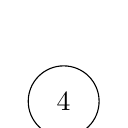
\begin{tikzpicture}[scale=0.15]
\tikzstyle{every node}+=[inner sep=0pt]
\draw [black] (37.5,-7.9) circle (3);
\draw (37.5,-7.9) node {$4$};
\end{tikzpicture}
\end{center}
Schritt 1: 1. Array-Element wird in leeren Heap eingefügt.\\

\begin{center}
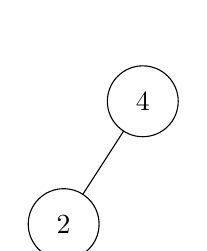
\begin{tikzpicture}[scale=0.15]
\tikzstyle{every node}+=[inner sep=0pt]
\draw [black] (37.5,-7.9) circle (3);
\draw [black] (30.8,-18.3) circle (3);
\draw (37.5,-7.9) node {$4$};
\draw (30.8,-18.3) node {$2$};
\draw [black] (35.88,-10.42) -- (32.42,-15.78);
\end{tikzpicture}
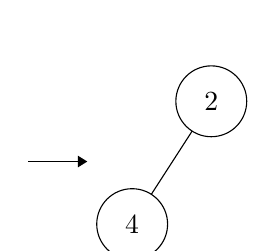
\begin{tikzpicture}[scale=0.15]
\tikzstyle{every node}+=[inner sep=0pt]
\draw [black] (22.00,-13.00) -- (27.00,-13.00);
\fill [black] (27.00,-13.00) -- (26.2,-12.5) -- (26.2,-13.5);
\draw [black] (37.5,-7.9) circle (3);
\draw [black] (30.8,-18.3) circle (3);
\draw (37.5,-7.9) node {$2$};
\draw (30.8,-18.3) node {$4$};
\draw [black] (35.88,-10.42) -- (32.42,-15.78);
\end{tikzpicture}
\end{center}
Schritt 2: 2. Array-Element wird in Heap eingefügt und Heap-Eingeschaft geprüft und hergestellt.\\

\begin{center}
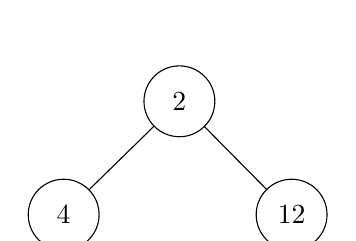
\begin{tikzpicture}[scale=0.15]
\tikzstyle{every node}+=[inner sep=0pt]
\draw [black] (34.5,-8.7) circle (3);
\draw (34.5,-8.7) node {$2$};
\draw [black] (24.7,-18.3) circle (3);
\draw (24.7,-18.3) node {$4$};
\draw [black] (44,-18.3) circle (3);
\draw (44,-18.3) node {$12$};
\draw [black] (32.36,-10.8) -- (26.84,-16.2);
\draw [black] (36.61,-10.83) -- (41.89,-16.17);
\end{tikzpicture}
\end{center}
Schritt 3: 3. Array-Element wird in Heap eingefügt. Heap-Eigenschaft erfüllt, kein Austausch.\\

\begin{center}
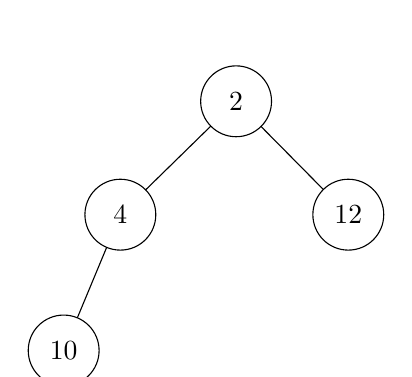
\begin{tikzpicture}[scale=0.15]
\tikzstyle{every node}+=[inner sep=0pt]
\draw [black] (34.5,-8.7) circle (3);
\draw (34.5,-8.7) node {$2$};
\draw [black] (24.7,-18.3) circle (3);
\draw (24.7,-18.3) node {$4$};
\draw [black] (44,-18.3) circle (3);
\draw (44,-18.3) node {$12$};
\draw [black] (19.9,-29.8) circle (3);
\draw (19.9,-29.8) node {$10$};
\draw [black] (32.36,-10.8) -- (26.84,-16.2);
\draw [black] (36.61,-10.83) -- (41.89,-16.17);
\draw [black] (23.54,-21.07) -- (21.06,-27.03);
\end{tikzpicture}
\end{center}
Schritt 4: 4. Array-Element in Heap einfügen. Heap-Eigenschaft erfüllt, kein Austausch.\\

\begin{center}
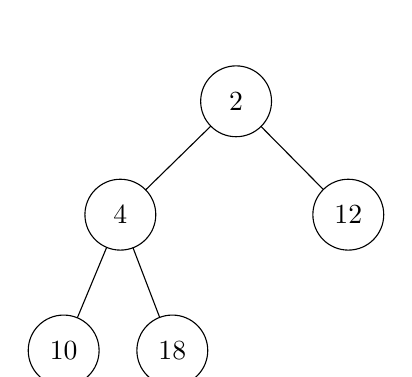
\begin{tikzpicture}[scale=0.15]
\tikzstyle{every node}+=[inner sep=0pt]
\draw [black] (34.5,-8.7) circle (3);
\draw (34.5,-8.7) node {$2$};
\draw [black] (24.7,-18.3) circle (3);
\draw (24.7,-18.3) node {$4$};
\draw [black] (44,-18.3) circle (3);
\draw (44,-18.3) node {$12$};
\draw [black] (19.9,-29.8) circle (3);
\draw (19.9,-29.8) node {$10$};
\draw [black] (29.1,-29.8) circle (3);
\draw (29.1,-29.8) node {$18$};
\draw [black] (32.36,-10.8) -- (26.84,-16.2);
\draw [black] (36.61,-10.83) -- (41.89,-16.17);
\draw [black] (23.54,-21.07) -- (21.06,-27.03);
\draw [black] (25.77,-21.1) -- (28.03,-27);
\end{tikzpicture}
\end{center}
Schritt 5: 5. Array-Element wird in Heap eingefügt. Heap-Eigenschaft erfüllt, kein Austausch.\\

\begin{center}
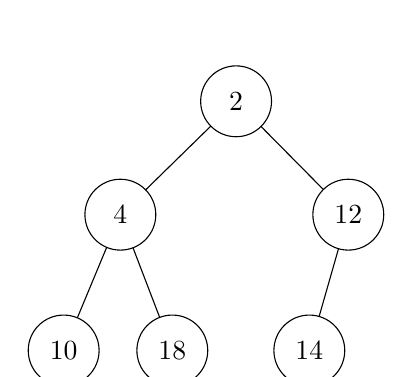
\begin{tikzpicture}[scale=0.15]
\tikzstyle{every node}+=[inner sep=0pt]
\draw [black] (34.5,-8.7) circle (3);
\draw (34.5,-8.7) node {$2$};
\draw [black] (24.7,-18.3) circle (3);
\draw (24.7,-18.3) node {$4$};
\draw [black] (44,-18.3) circle (3);
\draw (44,-18.3) node {$12$};
\draw [black] (19.9,-29.8) circle (3);
\draw (19.9,-29.8) node {$10$};
\draw [black] (29.1,-29.8) circle (3);
\draw (29.1,-29.8) node {$18$};
\draw [black] (40.7,-29.8) circle (3);
\draw (40.7,-29.8) node {$14$};
\draw [black] (32.36,-10.8) -- (26.84,-16.2);
\draw [black] (36.61,-10.83) -- (41.89,-16.17);
\draw [black] (23.54,-21.07) -- (21.06,-27.03);
\draw [black] (25.77,-21.1) -- (28.03,-27);
\draw [black] (43.17,-21.18) -- (41.53,-26.92);
\end{tikzpicture}
\end{center}
Schritt 6: 6. Array-Element wird eingefügt. Heap-Eigenschaft erfüllt, kein Austausch.\\

\begin{center}
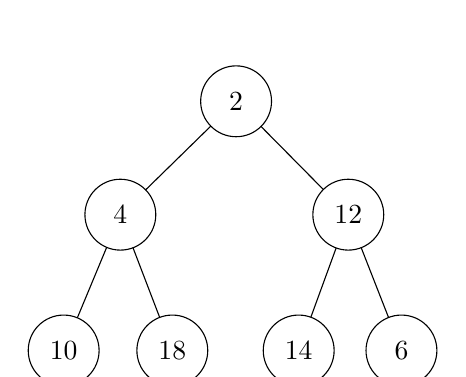
\begin{tikzpicture}[scale=0.15]
\tikzstyle{every node}+=[inner sep=0pt]
\draw [black] (34.5,-8.7) circle (3);
\draw (34.5,-8.7) node {$2$};
\draw [black] (24.7,-18.3) circle (3);
\draw (24.7,-18.3) node {$4$};
\draw [black] (44,-18.3) circle (3);
\draw (44,-18.3) node {$12$};
\draw [black] (19.9,-29.8) circle (3);
\draw (19.9,-29.8) node {$10$};
\draw [black] (29.1,-29.8) circle (3);
\draw (29.1,-29.8) node {$18$};
\draw [black] (39.8,-29.8) circle (3);
\draw (39.8,-29.8) node {$14$};
\draw [black] (48.5,-29.8) circle (3);
\draw (48.5,-29.8) node {$6$};
\draw [black] (32.36,-10.8) -- (26.84,-16.2);
\draw [black] (36.61,-10.83) -- (41.89,-16.17);
\draw [black] (23.54,-21.07) -- (21.06,-27.03);
\draw [black] (25.77,-21.1) -- (28.03,-27);
\draw [black] (42.97,-21.12) -- (40.83,-26.98);
\draw [black] (45.09,-21.09) -- (47.41,-27.01);
\end{tikzpicture}
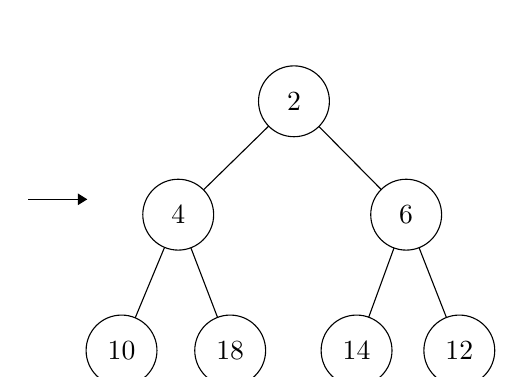
\begin{tikzpicture}[scale=0.15]
\tikzstyle{every node}+=[inner sep=0pt]
\draw [black] (12.00,-17.00) -- (17.00,-17.00);
\fill [black] (17.00,-17.00) -- (16.2,-16.5) -- (16.2,-17.5);
\draw [black] (34.5,-8.7) circle (3);
\draw (34.5,-8.7) node {$2$};
\draw [black] (24.7,-18.3) circle (3);
\draw (24.7,-18.3) node {$4$};
\draw [black] (44,-18.3) circle (3);
\draw (44,-18.3) node {$6$};
\draw [black] (19.9,-29.8) circle (3);
\draw (19.9,-29.8) node {$10$};
\draw [black] (29.1,-29.8) circle (3);
\draw (29.1,-29.8) node {$18$};
\draw [black] (39.8,-29.8) circle (3);
\draw (39.8,-29.8) node {$14$};
\draw [black] (48.5,-29.8) circle (3);
\draw (48.5,-29.8) node {$12$};
\draw [black] (32.36,-10.8) -- (26.84,-16.2);
\draw [black] (36.61,-10.83) -- (41.89,-16.17);
\draw [black] (23.54,-21.07) -- (21.06,-27.03);
\draw [black] (25.77,-21.1) -- (28.03,-27);
\draw [black] (42.97,-21.12) -- (40.83,-26.98);
\draw [black] (45.09,-21.09) -- (47.41,-27.01);
\end{tikzpicture}
\end{center}
Schritt 7: 7. Array-Element wird in Heap eingefügt und Heap-Eigenschaft geprüft und hergestellt.\\

\begin{center}
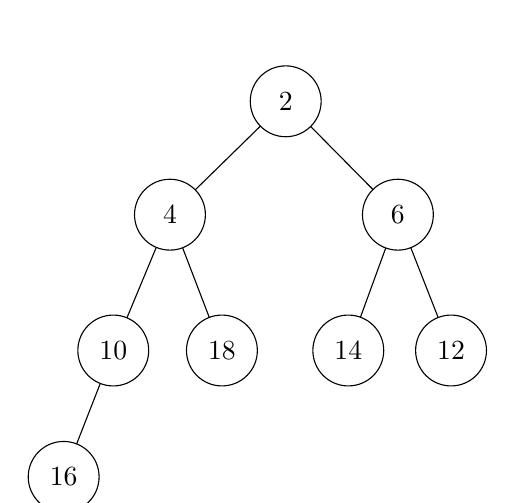
\begin{tikzpicture}[scale=0.15]
\tikzstyle{every node}+=[inner sep=0pt]
\draw [black] (34.5,-8.7) circle (3);
\draw (34.5,-8.7) node {$2$};
\draw [black] (24.7,-18.3) circle (3);
\draw (24.7,-18.3) node {$4$};
\draw [black] (44,-18.3) circle (3);
\draw (44,-18.3) node {$6$};
\draw [black] (19.9,-29.8) circle (3);
\draw (19.9,-29.8) node {$10$};
\draw [black] (29.1,-29.8) circle (3);
\draw (29.1,-29.8) node {$18$};
\draw [black] (39.8,-29.8) circle (3);
\draw (39.8,-29.8) node {$14$};
\draw [black] (48.5,-29.8) circle (3);
\draw (48.5,-29.8) node {$12$};
\draw [black] (15.7,-40.5) circle (3);
\draw (15.7,-40.5) node {$16$};
\draw [black] (32.36,-10.8) -- (26.84,-16.2);
\draw [black] (36.61,-10.83) -- (41.89,-16.17);
\draw [black] (23.54,-21.07) -- (21.06,-27.03);
\draw [black] (25.77,-21.1) -- (28.03,-27);
\draw [black] (42.97,-21.12) -- (40.83,-26.98);
\draw [black] (45.09,-21.09) -- (47.41,-27.01);
\draw [black] (18.8,-32.59) -- (16.8,-37.71);
\end{tikzpicture}
\end{center}
Schritt 8: 8. Array-Element wird in Heap eingefügt. Heap-Eigenschaft erfüllt, kein Austausch.\\

\begin{center}
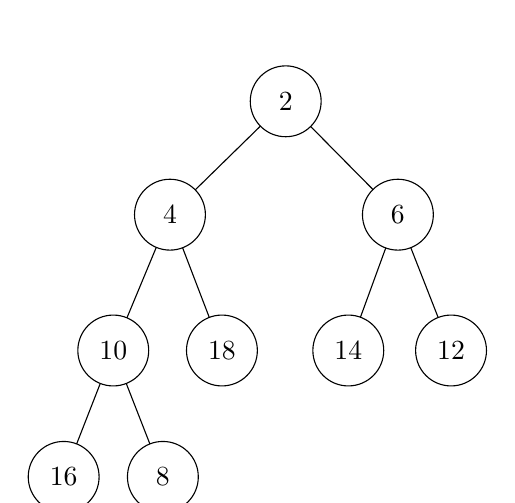
\begin{tikzpicture}[scale=0.15]
\tikzstyle{every node}+=[inner sep=0pt]
\draw [black] (34.5,-8.7) circle (3);
\draw (34.5,-8.7) node {$2$};
\draw [black] (24.7,-18.3) circle (3);
\draw (24.7,-18.3) node {$4$};
\draw [black] (44,-18.3) circle (3);
\draw (44,-18.3) node {$6$};
\draw [black] (19.9,-29.8) circle (3);
\draw (19.9,-29.8) node {$10$};
\draw [black] (29.1,-29.8) circle (3);
\draw (29.1,-29.8) node {$18$};
\draw [black] (39.8,-29.8) circle (3);
\draw (39.8,-29.8) node {$14$};
\draw [black] (48.5,-29.8) circle (3);
\draw (48.5,-29.8) node {$12$};
\draw [black] (15.7,-40.5) circle (3);
\draw (15.7,-40.5) node {$16$};
\draw [black] (24.1,-40.5) circle (3);
\draw (24.1,-40.5) node {$8$};
\draw [black] (32.36,-10.8) -- (26.84,-16.2);
\draw [black] (36.61,-10.83) -- (41.89,-16.17);
\draw [black] (23.54,-21.07) -- (21.06,-27.03);
\draw [black] (25.77,-21.1) -- (28.03,-27);
\draw [black] (42.97,-21.12) -- (40.83,-26.98);
\draw [black] (45.09,-21.09) -- (47.41,-27.01);
\draw [black] (18.8,-32.59) -- (16.8,-37.71);
\draw [black] (21,-32.59) -- (23,-37.71);
\end{tikzpicture}
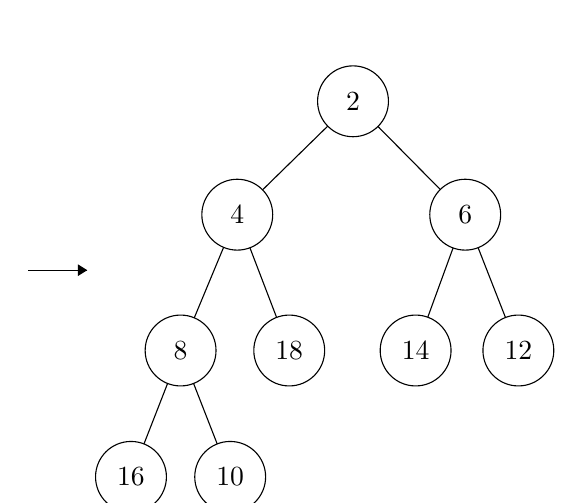
\begin{tikzpicture}[scale=0.15]
\tikzstyle{every node}+=[inner sep=0pt]
\draw [black] (7.00,-23.00) -- (12.00,-23.00);
\fill [black] (12.00,-23.00) -- (11.2,-22.5) -- (11.2,-23.5);
\draw [black] (34.5,-8.7) circle (3);
\draw (34.5,-8.7) node {$2$};
\draw [black] (24.7,-18.3) circle (3);
\draw (24.7,-18.3) node {$4$};
\draw [black] (44,-18.3) circle (3);
\draw (44,-18.3) node {$6$};
\draw [black] (19.9,-29.8) circle (3);
\draw (19.9,-29.8) node {$8$};
\draw [black] (29.1,-29.8) circle (3);
\draw (29.1,-29.8) node {$18$};
\draw [black] (39.8,-29.8) circle (3);
\draw (39.8,-29.8) node {$14$};
\draw [black] (48.5,-29.8) circle (3);
\draw (48.5,-29.8) node {$12$};
\draw [black] (15.7,-40.5) circle (3);
\draw (15.7,-40.5) node {$16$};
\draw [black] (24.1,-40.5) circle (3);
\draw (24.1,-40.5) node {$10$};
\draw [black] (32.36,-10.8) -- (26.84,-16.2);
\draw [black] (36.61,-10.83) -- (41.89,-16.17);
\draw [black] (23.54,-21.07) -- (21.06,-27.03);
\draw [black] (25.77,-21.1) -- (28.03,-27);
\draw [black] (42.97,-21.12) -- (40.83,-26.98);
\draw [black] (45.09,-21.09) -- (47.41,-27.01);
\draw [black] (18.8,-32.59) -- (16.8,-37.71);
\draw [black] (21,-32.59) -- (23,-37.71);
\end{tikzpicture}
\end{center}
Schritt 9: 9. und letztes Array-Element wird in Heap einfügen und Heap-Eigenschaft wird geprüft und hergestellt. Min-Heap ist vollständig erstellt.

\paragraph{b)}
Wie sieht der Heap aus, wenn Sie eine \textsc{ExtractMin} Operation ausgeführt und dann die Heapeigenschaft wieder hergestellt haben? \\

Nach ExtractMin:
\begin{center}
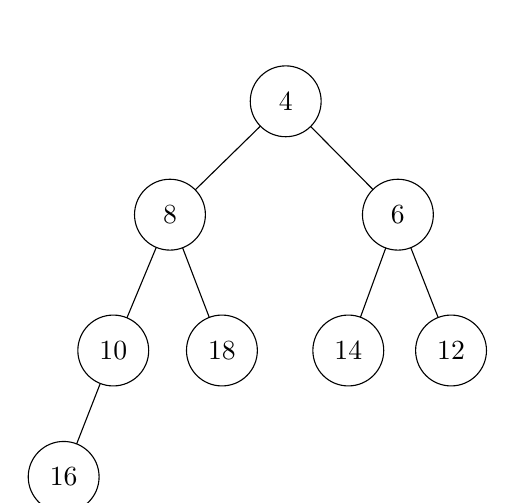
\begin{tikzpicture}[scale=0.15]
\tikzstyle{every node}+=[inner sep=0pt]
\draw [black] (34.5,-8.7) circle (3);
\draw (34.5,-8.7) node {$4$};
\draw [black] (24.7,-18.3) circle (3);
\draw (24.7,-18.3) node {$8$};
\draw [black] (44,-18.3) circle (3);
\draw (44,-18.3) node {$6$};
\draw [black] (19.9,-29.8) circle (3);
\draw (19.9,-29.8) node {$10$};
\draw [black] (29.1,-29.8) circle (3);
\draw (29.1,-29.8) node {$18$};
\draw [black] (39.8,-29.8) circle (3);
\draw (39.8,-29.8) node {$14$};
\draw [black] (48.5,-29.8) circle (3);
\draw (48.5,-29.8) node {$12$};
\draw [black] (15.7,-40.5) circle (3);
\draw (15.7,-40.5) node {$16$};
\draw [black] (32.36,-10.8) -- (26.84,-16.2);
\draw [black] (36.61,-10.83) -- (41.89,-16.17);
\draw [black] (23.54,-21.07) -- (21.06,-27.03);
\draw [black] (25.77,-21.1) -- (28.03,-27);
\draw [black] (42.97,-21.12) -- (40.83,-26.98);
\draw [black] (45.09,-21.09) -- (47.41,-27.01);
\draw [black] (18.8,-32.59) -- (16.8,-37.71);
\end{tikzpicture}
\end{center}

Durch Extractmin wird die Wurzel entfernt, da Wurzel das kleinste Element ist.\\
Dann wird 10 zur Wurzel und sinkt nach unten.\\
Dabei wird erst 10  mit 4 getauscht und anschließend 10 mit 8 vertauscht.\\

\paragraph{c)}
Fügen Sie das neue Element $3$ zu dem Heap (aus b) hinzu. \\

\begin{center}
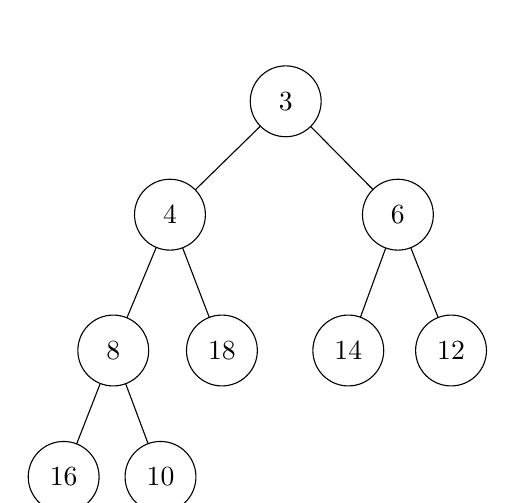
\begin{tikzpicture}[scale=0.15]
\tikzstyle{every node}+=[inner sep=0pt]
\draw [black] (34.5,-8.7) circle (3);
\draw (34.5,-8.7) node {$3$};
\draw [black] (24.7,-18.3) circle (3);
\draw (24.7,-18.3) node {$4$};
\draw [black] (44,-18.3) circle (3);
\draw (44,-18.3) node {$6$};
\draw [black] (19.9,-29.8) circle (3);
\draw (19.9,-29.8) node {$8$};
\draw [black] (29.1,-29.8) circle (3);
\draw (29.1,-29.8) node {$18$};
\draw [black] (39.8,-29.8) circle (3);
\draw (39.8,-29.8) node {$14$};
\draw [black] (48.5,-29.8) circle (3);
\draw (48.5,-29.8) node {$12$};
\draw [black] (15.7,-40.5) circle (3);
\draw (15.7,-40.5) node {$16$};
\draw [black] (23.9,-40.5) circle (3);
\draw (23.9,-40.5) node {$10$};
\draw [black] (32.36,-10.8) -- (26.84,-16.2);
\draw [black] (36.61,-10.83) -- (41.89,-16.17);
\draw [black] (23.54,-21.07) -- (21.06,-27.03);
\draw [black] (25.77,-21.1) -- (28.03,-27);
\draw [black] (42.97,-21.12) -- (40.83,-26.98);
\draw [black] (45.09,-21.09) -- (47.41,-27.01);
\draw [black] (18.8,-32.59) -- (16.8,-37.71);
\draw [black] (20.95,-32.61) -- (22.85,-37.69);
\end{tikzpicture}
\end{center}
Das Element 3 wird am Ende des Arrays angehängt und anschließend die Heapeigenschaft getestet.\\
3 steigt dabei nach dem Vergleich mit der 10, 8 und 4 bis zur Wurzel auf.\\

\paragraph{d)}
Analysieren Sie in $\mathcal{O}$-Notation die Laufzeit der Methode \textsc{ExtractMax}, die das maximale Element aus einem Min-Heap $S$ der Größe $n$ löscht. \\

ExtractMax benötigt n - 1 Schritte, um alle Blätter des Heaps zu finden und dann noch einmal maximal $2^{Hoehe(H)}+1$ Schritte für den Vergleich der Blätter, das Finden und das Löschen des Maximums.\\
Weil die Höhe des Heaps bei jeder nächsten Zweierpotenz um 1 steigt, haben wir $Hoehe(H) = \lfloor \log_2 n \rfloor$, also die Laufzeit $T(n) = n-1 + 2^{Hoehe(H)}+1 \leq n+2^{\log_2 n} = n + n = 2n \Rightarrow \mathcal{O}(n)$.

%----------------------------------------------------------------------------
\subsection{Eine Erweiterung von Heapsort}
In der Vorlesung haben Sie das Sortierverfahren Heapsort kennengelernt. Wir betrachten nun eine Erweiterung dieses Verfahrens, das sogenannte \emph{$k$-Heapsort}. Dabei ist $k\ge2$ eine natürliche Zahl. Bei diesem Verfahren benutzt man statt einem Binärbaum einen $k$-nären Baum, bei dem jeder Knoten höchstens $k$ Kinder hat. Deshalb heißt der korrespondierende Heap $k$-Heap. 

\paragraph{a)}
Wie kann man einen $k$-Heap als ein Array repräsentieren? Wie effizient ist es, die Kinder bzw. den Elternknoten eines gegebenen Knoten zu finden? \\

Array A$[a_0 ..... a_n]$

Root: $a_0$\\
1st Level: $a_1 ..... a_{2+k}$ \\
2nd Level: $a_{1+k} ...... a_{2+k+k^2}$\\
.\\
.\\
.\\
nth Level: $a_{1+ \sum_{i=1}^{n-1} {k^i}} ... a_{\sum_{i=1}^{n} {k^i}}$\\

Parent nodes of i: $\lfloor{(i-1)/k}\rfloor$\\
Child nodes j of i: $i*k +j$ ($1\leq j \leq k$)\\


\paragraph{b)} Geben Sie die Höhe eines $k$-Heaps an, wenn dieser $n$ Elemente enthält. \\

h = $\lceil log_k((n * k) - (n + 1))\rceil - 1$

\paragraph{c)} 
Geben Sie Pseudocode für effiziente Implementierungen der Methoden \texttt{Insert} und \texttt{ExtractMin} an. Analysieren Sie die Komplexität der beiden Methoden in Abhängigkeit von $n$ und $k$. \\

A = Array, X = Element, I = Index, k

\begin{lstlisting}
Insert(A, X, k) {
    Increase length of A by 1
    Insert X at A[length(A)]
    HeapUp(A, length(A) - 1, k)
}

HeapUp(Array A, i, k) {
    
    while (i not root){
    
      if (array[i] > array[parent-position] {
          Swap A[i] and A[parent-position]
          i = parent
          parent = (i-1)/k
      }
      else 
      	break
	}
}

\end{lstlisting}
Complexity:\\
Because we need a comparison for each tree-level: Insert() $\in \mathcal{O}(log_k((n*k) - (n+1))$\\
	
\begin{lstlisting}
ExtractMin(Array A)
{
	Extract root
    Set length(A)-1 (last element) as new root
    Shorten array by 1
    HeapDown(A, root)
}

HeapDown(array A, node n)
{
	for (n not leaf){
    	compare n to its childs 1 - k step by step
        	if(n < child){
            	swap (n, child)                
            }
         HeapDown(A, child)
             
    }
}

\end{lstlisting}
Complexity:\\
We need k comparisons on every level, thats why extractMin() $\in \mathcal{O}(3 log_k(n*k - n) $.\\

%----------------------------------------------------------------------------
\subsection{Zwei-Drittel-Sortieren}
Eine alternative Methode, um ein Array $A$ der Länge $n$ zu sortieren, ist die Folgende:

\begin{algorithm}[H]
	\If{$A[left] > A[right]$} {
		exchange $A[left]$ and $A[right]$ \;
	}
	\If{$left + 1 \ge right$} {
		\Return \;
	}
	$k \longleftarrow \left\lfloor \frac{right - left + 1}3 \right\rfloor$ \;
	\texttt{ZweiDrittelSortieren}($A$, $left$, $right-k$)\;
	\texttt{ZweiDrittelSortieren}($A$, $left+k$, $right$)\;
	\texttt{ZweiDrittelSortieren}($A$, $left$, $right-k$)\;
 \caption{\texttt{ZweiDrittelSortieren}($A$, $left$, $right$)}
 \label{algo:ZweiDrittelSortieren}
\end{algorithm}

\paragraph{a)}
Argumentieren Sie, dass \texttt{ZweiDrittelSortieren}($A$, $1$, $n$) das Array $A[1..n]$ korrekt sortiert. \\

Argumentation, dass Zwei-Drittel-Sortieren korrekt ist, mithilfe von Induktion über die Länge des sortierten Teilarrays k: ($right-left+1$).\\
Für Länge 1 ist das Array immer sortiert, für Länge 2 muss einmal verglichen und gegebenenfalls ausgetauscht werden.\\
\\
Für Längen > 2 sei $k = (right-left+1)/3$.\\
Betrachte nun die k größten Elemente des Arrays von left bis right.\\
$m \leq k$ Elemente sind in den ersten zwei Dritteln des Arrays und gleichzeitig sind $m$ die größten Elemente dieses Teilarrays.\\
Nach der ersten Rekursion, die das Teilarray korrekt sortiert hat (Induktionsvoraussetzung korrekt), befinden sich diese $m$ Elemente im Teilarray A[$right-k-m+1$]...A[$right-k$] mit der Eigenschaft $right-k-m+1 \geq left+k$.\\
\\
Das mittlere Drittel besteht aus mindestens k Elementen und die k größten Elemente befinden sich zwischen $left + k$ und $right$, also sind diese auch nach dem zweiten Aufruf korrekt sortiert.\\
Im letzten Drittel des Arrays die (übrigens) $\leq$ k größten Elemente, welche im letzten rekursiven Aufruf sortiert werden.

\paragraph{b)}
Analysieren Sie die Laufzeit von \texttt{ZweiDrittelSortieren} im worst-case. Geben Sie Ihre Angaben in $\mathcal{O}$-Notation an. \\

Worst-Case: In jedem Rekursionsschritt werden zwei Elemente ($left$, $right$ des jeweiligen Teilarrays) getauscht werden und anschließend weiter gedrittelt, daher $T(n) = 3*T(\frac{n}{3})+2$.\\
\\
Mastertheorem:\\
$a = 3,$ $b= 3,$ $f(n) = 2*n^0$\\
$f(n) = 2*n^{1-1} = 2*n^{\log_3(3)-1} \in \mathcal{O}(n^{\log_3(3)-\epsilon})$ wobei $\epsilon = 1$\\
$\Rightarrow T(n) \in \Theta(n^{\log_3(3)}) \in \Theta(n^1) \in \Theta(n)$

\paragraph{c)}
Ist Zwei-Drittel-Sortieren im worst-case effizienter als Insertsort, Minimumsuche+Austauschen, Quicksort oder Heapsort? Alle Antworten sollten jeweils ausreichend begründet werden. \\

Insertion Sort Worst-Case Laufzeit:\\
$T(n) = \frac{n^2+n}{2} = \mathcal{O}(n^2)$, zwei-Drittel-Sortieren ist also deutlich schneller.\\
Minimumsuche + Austausch hat eine Worst-Case Laufzeit von $T(n) = \frac{n^2+n}{2} = \mathcal{O}(n^2)$, zwei-Drittel-Sortieren ist also deutlich schneller.\\
Quicksort hat die Worst-Case Laufzeit $\mathcal{O}(n^2)$, zwei-Drittel-Sortieren ist also deutlich schneller.\\
Heapsort hat die Worst-Case Laufzeit $\mathcal{O}(n \log n)$, zwei-Drittel-Sortieren ist also etwas schneller.

%----------------------------------------------------------------------------------------
\newpage
\section{Blatt 05}
%----------------------------------------------------------------------------
\subsection{Bucketsort}
Gegeben seien $n$ Zahlen im Bereich $[0,\dots, n^k-1]$ für ein festes $k\in \mathbb N$.
Zeigen Sie, dass mittels Bucketsort die Zahlen mit einer Worstcase-Laufzeit von $O(n)$ sortiert werden können.\\
\textit{Hinweis: Stellen Sie die Zahlen zur Basis $n$ dar.} \\

Bucketsort sortiert jede Zahl im ersten Schritt an der letzten Stelle in das passende von 10 Buckets.\\
Für k = 1, 2, ... steigen die Längen der Zahlen für jeweiliges n>1 grob um 2*length($n^{k-1} - 1$).\\
Also wird für höheres k häufiger in Buckets einsortiert wegen der Stellenlänge der höchsten Zahl im Array, genau der Stellenanzahl $n^k - 1$.\\
Die Länge hierzu lässt sich mit $\prod_{i=Stellenlaenge von n^k - 1}^{k} i$ bei festem k bestimmen, was $Stellenlaenge * k!$ ist.\\
Wir haben also $10 * Stellenlaenge * k! * n$ Suchläufe und da k fest ist, sowie auch die Stellenlänge kann dies als Konstante c dargestellt werden: $c * n \in \mathcal{O}(n)$.\\


%----------------------------------------------------------------------------
\subsection{Mediansuche in Linearzeit}

\paragraph{a)}
In der Vorlesung haben Sie gelernt, wie Sie den Median von fünf
Zahlen mit 7 Vergleichen bestimmen können. Verallgemeinern Sie
dieses (rekursive) Vorgehen für Eingaben ungerader Länge. Geben Sie
die Anzahl benötigter Vergleiche für Listen der Länge $n$, mit $n\in \{7,9,11,13,15,17\}$ an. \\

\begin{enumerate}
\item Aufteilen der Menge in Paare $\rightarrow$ am Ende soll eine Zahl übrig bleiben. Die Zahlenpaare werden miteinander verglichen ($\lfloor \dfrac{n}{2} \rfloor$ Vergleiche)
\item Bestimme das Minimum unter allen Zahlen, die im Zahlenpaar kleiner waren im Vergleich($\lfloor \dfrac{n}{2} \rfloor -1$ Vergleiche)
\item das gleiche für das Maximum ($\lfloor \dfrac{n}{2} \rfloor -1$ Vergleiche)
\item Minimum und Maximum aus dem Array nehmen und den Algorithmus auf das Array Größe n-2 aufrufen (V(n-2) Vergleiche)
\end{enumerate}

Es folgt: $V(n)=\lfloor \dfrac{n}{2} \rfloor + 2*(\lfloor \dfrac{n}{2} \rfloor -1) +V(n-2) $ \\

Rekursionsende: V(5)=7 \\

Daraus folgt folgende Anzahl an Vergleichen für Listen der Länge n: \\

\begin{tabular}{|c|c|}
\hline
n & V(n) \\\hline
7 & $\lfloor \dfrac{7}{2} \rfloor + 2*(\lfloor \dfrac{7}{2} \rfloor -1) +V(5) = 14$ \\\hline
9 & $\lfloor \dfrac{9}{2} \rfloor + 2*(\lfloor \dfrac{9}{2} \rfloor -1) +V(7) = 24$ \\\hline
11 & $\lfloor \dfrac{11}{2} \rfloor + 2*(\lfloor \dfrac{11}{2} \rfloor -1) +V(9) = 37$ \\\hline
13 & $\lfloor \dfrac{13}{2} \rfloor + 2*(\lfloor \dfrac{13}{2} \rfloor -1) +V(11) = 53$ \\\hline
15 & $\lfloor \dfrac{15}{2} \rfloor + 2*(\lfloor \dfrac{15}{2} \rfloor -1) +V(13) = 72$ \\\hline
17 & $\lfloor \dfrac{17}{2} \rfloor + 2*(\lfloor \dfrac{17}{2} \rfloor -1) +V(15) = 94$ \\\hline
\end{tabular}

\paragraph{b)}
Für die Laufzeitanalyse der Medianbestimmung ergab sich bei einer Unterteilung in Fünfergruppen die folgende Rekursionsgleichung:
\[
T(n) \leq T
\left(
  \frac{n}{5}
\right) + T
\left(
  \frac{7}{10}n
\right) + c \cdot n
\]

\paragraph{I)}
Geben Sie eine möglichst gute Konstante $c$ an. \\

z.z. $T(n) \leq T(\dfrac{n}{5})+T(\dfrac{7n}{10} *n)+c_{1} * n$ \\

in Vorlesung bewiesen, dass $T(n) \leq c_{2} * \dfrac{n}{5} + c_{2} * \dfrac{7n}{10}$ ist; $d= \dfrac{c_{2}}{10}$ \\

damit gilt: $d=c_{1}$ \\

somit ist $c_{2}* \dfrac{n}{5} + c_{2} * \dfrac{7n}{10} + d*n = \dfrac{n}{5} + \dfrac{7n}{10} + c_{1}*n$ \\

$\dfrac{n}{5} + \dfrac{7n}{10} + c_{1}*n$ \\

$= \dfrac{9n}{10} + d*n$ \\

$\Rightarrow c_{2}=1$ \\

$\Rightarrow d= \dfrac{1}{10}$ \\

$\Rightarrow c_{1} = \dfrac{1}{10}$

\paragraph{II)} 
Wie verändert sich die Rekursionsgleichung, wenn die Liste in Siebener- statt in Fünfergruppen geteilt wird?
Geben Sie auch hier eine möglichst gute Abschätzung der Konstante $c$ an. \\

z.z. $T(n) \leq T(\dfrac{n}{7})+T( \dfrac{10}{14}*n) + c_{1} * n$ \\

dieselbe Berechnung wie oben \\

$\dfrac{n}{7} + \dfrac{10n}{14} + d*n$ \\

$= \dfrac{12n}{14} + d*n$ \\

$\Rightarrow c_{2}=2$ \\

$\Rightarrow d= \dfrac{2}{14}$ \\

$\Rightarrow c_{1} = \dfrac{2}{14}$

%----------------------------------------------------------------------------
\subsection{Median in sortierten Arrays}
Seien $A[1..n]$ und $B[1..n]$ zwei sorrtierte Arrays der Größe $n$.

\paragraph{a)}
Beschreiben Sie einen Algorithmus, der den Median aller $2n$ Elemente aus A und B in Zeit $O(\log n)$ findet. \\

\begin{algorithm}[H]
\SetAlgoLined
\textbf{Data} Array A, Array B (beide mit Länge n) \\
\textbf{Result} Median m aller 2n Elemente aus A und B \\
make new Array C mit Größe 2n \\
int k = 0 (Position in A) \\
int l = 0 (Position in B) \\
\textbf{for} 0 to 2n-1 do \\
\textbf{if} A[k] $\leq$ B[l] \\
C[i] $\leftarrow$ A[k] \\
k++ \\
\textbf{else} \\
C[i] $\leftarrow$ B[l] \\
l++ \\
end if \\
end for \\
int $d= \dfrac{2n}{2} -1$ \\
int $m = \dfrac{C[d]+C[d+1]}{2} $ \\
return m
\end{algorithm}

\paragraph{b)}
Begründen Sie die Laufzeit und die Korrektheit Ihres Algorithmus. \\

Laufzeit O(n)

%----------------------------------------------------------------------------
\subsection{Konvexe Hülle}
Gegeben sei eine Menge $M=\{(x_i, y_i)\in \mathbb Q^2 \mid 1 \leq i \leq n\}$. Die konvexe Hülle $\operatorname{conv}(M)$ einer Menge $M$ ist der kleinste Polyeder der alle Punkte in $M$ enthält. Eine einfache Repräsentation der konvexen Hülle ist die kleinste Menge $N \subseteq M$ von Punkten, so dass $\operatorname{conv}(N)=\operatorname{conv}(M)$. Bildlich gesprochen: die \textit{Eckpunkte} der Menge $M$. Eine \textit{zyklische Sortierung} der Eckpunkte ist eine Ordnung der Punkte in $N$ so, dass beim Ablaufen der Punkte nach der Sortierung ein Weg um das Polygon entsteht.

\medskip\noindent Nehmen Sie an, dass Sie einen Algorithmus haben der in Zeit $T(n)$, gegeben eine Menge $M$ (wie oben), eine zyklische Sortierung der Eckpunkte der konvexen Hülle ausgibt. Zeigen Sie, dass $\Omega(n \log n)$ eine untere Schranke für die worst-case Laufzeit des Algorithmus ist.

\begin{figure}[htp!]
\begin{center}
  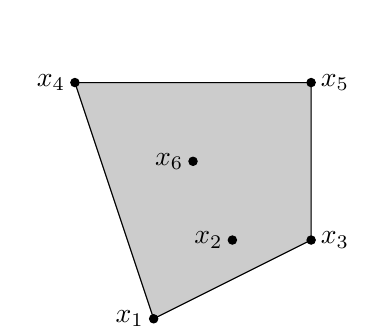
\begin{tikzpicture}
    \draw[fill] (0,0) circle(1.5pt) node[left]{$x_1$};
    \draw[fill] (1,1) circle(1.5pt) node[left]{$x_2$};
    \draw[fill] (.5,2) circle(1.5pt) node[left]{$x_6$};
    \draw[fill] (2,1) circle(1.5pt) node[right]{$x_3$};
    \draw[fill] (-1,3) circle(1.5pt) node[left]{$x_4$};
    \draw[fill] (2,3) circle(1.5pt) node[right]{$x_5$};   
    \draw (0,0) -- (2,1) -- (2,3) -- (-1,3)-- (0,0);
    \draw[fill=black, opacity=.2] (0,0) -- (2,1) -- (2,3) -- (-1,3)-- (0,0);
  \end{tikzpicture}\\
\end{center}
\caption{Der Algorithmus erhält die Punktemenge $\{x_1,\dots,x_6\}$ und gibt die Punkteliste $(x_1,x_4,x_5,x_3)$ aus. Der grau gefärbte Bereich ist die konvexe Hülle.
}\end{figure}

geg: 
\begin{itemize}
\item Algorithmus in Zeit T(n)
\item Menge $M= {(x_{i},y_{i}) \in \mathbb{Q}^{2} | 1 \leq i \leq n}$
\item zyklische Sortierung der Eckpunkte der konvexen Hülle
\end{itemize} \\

z.z. $\Omega$ (n log n) ist eine untere Schranke für worst-case Laufzeit des Algorithmus \\

Probleme:
\begin{enumerate}
\item konvexe Hülle bestimmen
\item Verwendung des vergleichsbasierenden Sortierens; läuft also bestenfalls auch n log n
\end{enumerate} \\

Problemlösung:
\begin{itemize}
\item transformieren einer Instanz I(B) (ein Array X) zu einer Instanz I(A)\\
generieren zu jeder Zahl aus X einen Punkt $(x_{i},x_{i}^{2})$ \\
läuft in Zeit O(n) $\rightarrow$ einmaliges Durchlaufen des Arrays und währenddessen das Erzeugen des jeweiligen Punktes 
\item man erhält n Punkte, welche alle auf einer Parabel liegen \\
die konvexe Hülle besteht dann genau aus diesen Punkten
\item Algorithmus soll Instanz I(A)lösen \\
in angegebener Zeit T(n)
\item Lösung soll nun zu einer Lösung von Instanz I(B) transformiert werden \\
soll eine sortierte Liste werden \\
zuerst wird der Eckpunkt mit der kleinsten x-Koordinate ausgewählt \\
x- Koordinate dieses Punktes kommt an die erste Stelle des Ergebnisarrays \\
alle folgenden Werte werden von der Parabel (von links nach rechts) abgelesen
\end{itemize}


%----------------------------------------------------------------------------
\subsection{Untere Schranke}
Sei $A$ eine sortierte Liste der Größe $n$.

\paragraph{a)}
Das erste Problem besteht daraus, zu entscheiden, ob in der Liste $A$ Duplikate vorkommen.
Beweisen Sie, dass $n-1$ eine untere Schranke für die Anzahl der Vergleiche ist, die man dafür braucht. \\

3 Fälle:
\begin{enumerate}
\item Fall \\
Abgleichen des ersten Elementes mit der Liste und finden des erstes Elementes an der letzten Stelle in der Liste. Dann muss man n-1 mal vergleichen, also das Erste mit jedem Element der Liste, außer mit sich selbst.
\item Fall \\
Abgleichen des ersten Elementes mit der Liste und finden des erstes Elementes an der letzten Stelle in der Liste. Hierbei muss man n-(n-Anzahl Stellen vor Listenende) vergleichen. Da aber $\Omega(n-(n-1)) \in \Omega(n-1)$, auch hier untere Grenze von $\Omega(n-1)$
\item Fall \\
\end{enumerate}

\paragraph{b)}
Das zweite Problem ist es, zu entscheiden, ob in der Liste $A$ ein beliebiger Wert $x$ vorkommt.
Beweisen Sie, dass im worst-case $\Omega(\log n)$ Vergleiche dafür benötigt werden (unabhängig vom verwendeten
Algorithmus). \\

%----------------------------------------------------------------------------------------
\newpage
\section{Blatt 06}
%----------------------------------------------------------------------------
\subsection{AVL-Bäume}

\paragraph{a)}
 Fügen Sie die Zahlen 63, 30, 36, 31, 12, 50, 35, 5, 27, 59, 43, 17 (in dieser Reihenfolge) in einen (zu Beginn leeren) AVL-Baum ein. Sie dürfen die Schritte, in denen nicht rotiert, sondern nur eingefügt wird, zusammenfassen. \\
 
\textbf{Schritt 1} 

\begin{center}
 \begin{tikzpicture}[level/.style={sibling distance=60mm/#1}]
\node [circle,draw] (z){$63$}
\end{tikzpicture}}
 \end{center} 

\textbf{Schritt 2,3} 

\begin{center}
\begin{tikzpicture}[level/.style={sibling distance=60mm/#1}]
\node [circle,draw] (z){$63$}
  child {node [circle,draw] (a) {$30$}  
    child {node [circle,draw] (b) {}} 
    child {node [circle,draw] (c) {$36$}}  
  }
  child {node [circle,draw] (d) {}}  
\end{tikzpicture}}
\end{center} 

$bal(63)=-2,bal(30)=1$ \\
$\Rightarrow$ VZ ungleich \\
$\Rightarrow$ Doppelrotation \\

\textbf{Schritt 4}

\begin{center}
\begin{tikzpicture}[level/.style={sibling distance=60mm/#1}]
\node [circle,draw] (z){$63$}
  child {node [circle,draw] (a) {$30$}  
    child {node [circle,draw] (c) {$36$}}  
    child {node [circle,draw] (b) {}} 
  }
  child {node [circle,draw] (d) {}}  
\end{tikzpicture}}
\end{center} 

\begin{center}
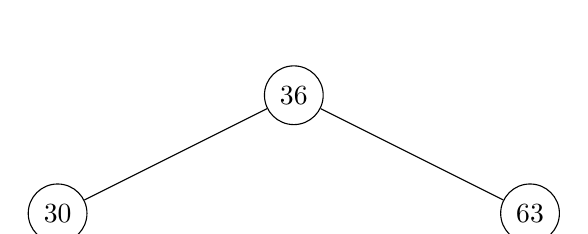
\begin{tikzpicture}[level/.style={sibling distance=60mm/#1}]
\node [circle,draw] (z){$36$}
  child {node [circle,draw] (a) {$30$}
  }
  child {node [circle,draw] (j) {$63$}
};
\end{tikzpicture}}
\end{center}

\textbf{Schritt 5,6,7,8,9,10,11}

\begin{center}
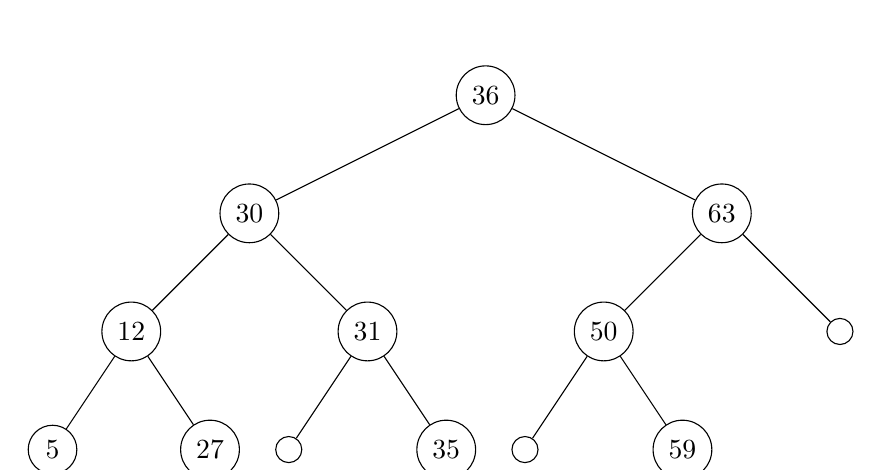
\begin{tikzpicture}[level/.style={sibling distance=60mm/#1}]
\node [circle,draw] (z){$36$}
  child {node [circle,draw] (a) {$30$}
    child {node [circle,draw] (b) {$12$}
       child {node [circle,draw] (c) {$5$}}
       child {node [circle,draw] (d) {$27$}}
    }
    child {node [circle,draw] (e) {$31$}
       child {node [circle,draw] (j) {}} 
       child {node [circle,draw] (d) {$35$}}
    }
  }
  child {node [circle,draw] (g) {$63$}
    child {node [circle,draw] (h) {$50$}
       child {node [circle,draw] (l) {}} 
       child {node [circle,draw] (i) {$59$}}
    }
    child {node [circle,draw] (k) {}} 
  };
\end{tikzpicture}}
\end{center}

$bal(63)=-2,bal(50)=1$\\
$\Rightarrow$ VZ ungleich \\
$\Rightarrow$ Doppelrotation \\

\textbf{Schritt 12}

\begin{center}
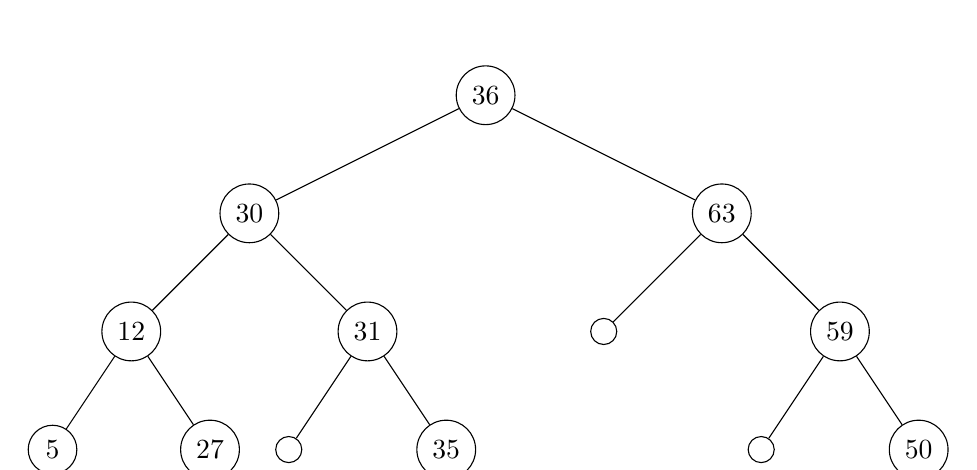
\begin{tikzpicture}[level/.style={sibling distance=60mm/#1}]
\node [circle,draw] (z){$36$}
  child {node [circle,draw] (a) {$30$}
    child {node [circle,draw] (b) {$12$}
       child {node [circle,draw] (c) {$5$}}
       child {node [circle,draw] (d) {$27$}}
    }
    child {node [circle,draw] (e) {$31$}
       child {node [circle,draw] (j) {}} 
       child {node [circle,draw] (d) {$35$}}
    }
  }
  child {node [circle,draw] (g) {$63$}
    child {node [circle,draw] (k) {}} 
    child {node [circle,draw] (h) {$59$}
       child {node [circle,draw] (l) {}} 
       child {node [circle,draw] (i) {$50$}}
    }
  };
\end{tikzpicture}}
\end{center}

\begin{center}
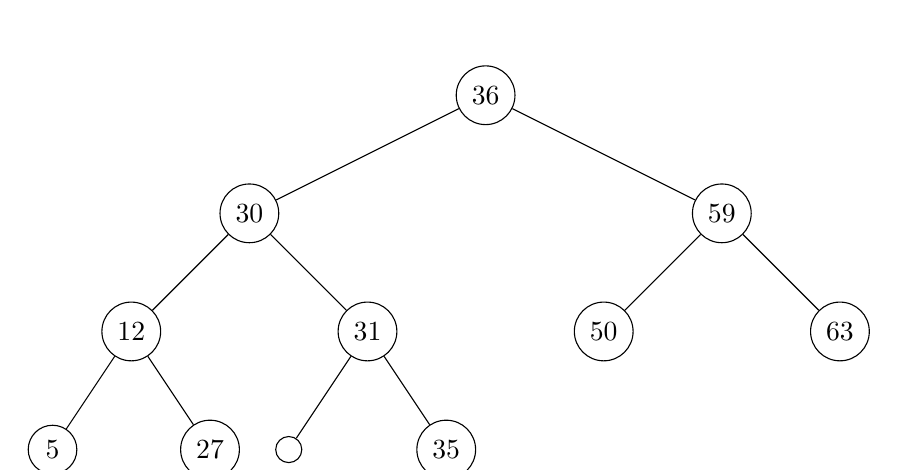
\begin{tikzpicture}[level/.style={sibling distance=60mm/#1}]
\node [circle,draw] (z){$36$}
  child {node [circle,draw] (a) {$30$}
    child {node [circle,draw] (b) {$12$}
       child {node [circle,draw] (c) {$5$}}
       child {node [circle,draw] (d) {$27$}}
    }
    child {node [circle,draw] (e) {$31$}
       child {node [circle,draw] (j) {}} 
       child {node [circle,draw] (f) {$35$}}
    }
  }
  child {node [circle,draw] (g) {$59$}
    child {node [circle,draw] (h) {$50$}}
    child {node [circle,draw] (i) {$63$}}
  };
\end{tikzpicture}}
\end{center}

\textbf{Schritt 13,14}

\begin{center}
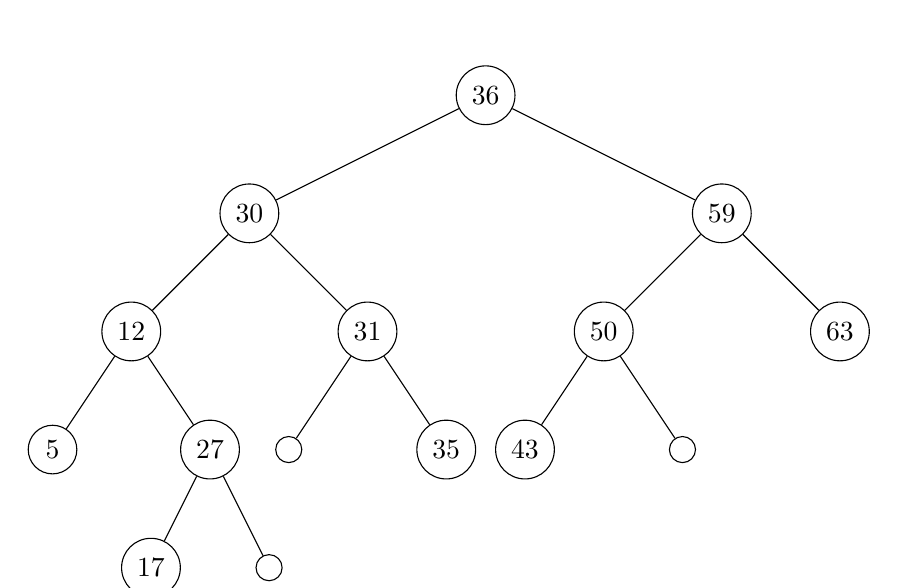
\begin{tikzpicture}[level/.style={sibling distance=60mm/#1}]
\node [circle,draw] (z){$36$}
  child {node [circle,draw] (a) {$30$}
    child {node [circle,draw] (b) {$12$}
       child {node [circle,draw] (c) {$5$}}
       child {node [circle,draw] (d) {$27$}
          child {node [circle,draw] (e) {$17$}}
          child {node [circle,draw] (l) {}} 
       }
    }
    child {node [circle,draw] (f) {$31$}
       child {node [circle,draw] (m) {}} 
       child {node [circle,draw] (g) {$35$}}
    }
  }
  child {node [circle,draw] (h) {$59$}
    child {node [circle,draw] (i) {$50$}
       child {node [circle,draw] (j) {$43$}}
       child {node [circle,draw] (n) {}} 
    }
    child {node [circle,draw] (k) {$63$}}
  };
\end{tikzpicture}}
\end{center}

$|bal(u) \leq 1|: \forall n$, n Knoten $\Rightarrow$ fertig

\paragraph{b)} 
Löschen Sie die Zahlen 36, 43 wieder aus dem Baum. Geben Sie die Schritte an. \\

Lösche 36 und hefte 43 an Baum

\begin{center}
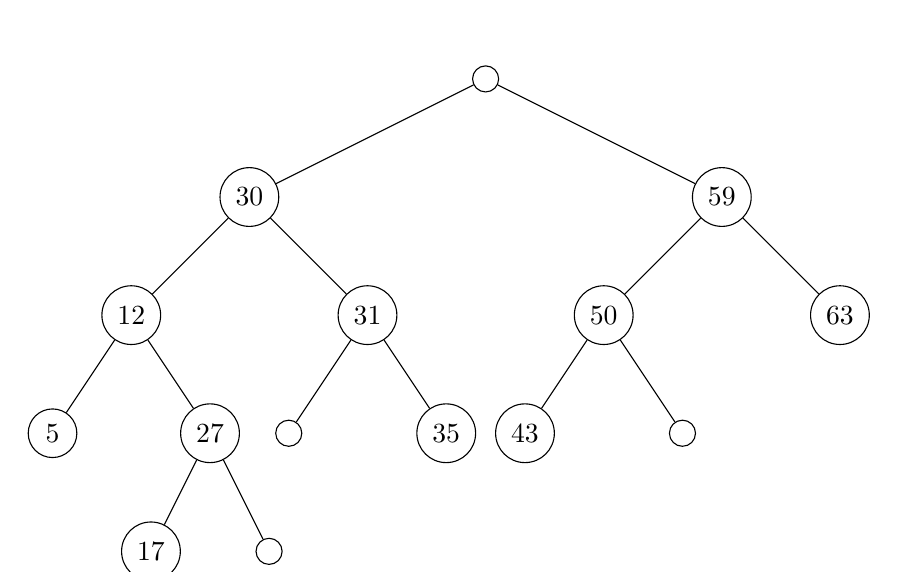
\begin{tikzpicture}[level/.style={sibling distance=60mm/#1}]
\node [circle,draw] (z){$ $}
  child {node [circle,draw] (a) {$30$}
    child {node [circle,draw] (b) {$12$}
       child {node [circle,draw] (c) {$5$}}
       child {node [circle,draw] (d) {$27$}
          child {node [circle,draw] (e) {$17$}}
          child {node [circle,draw] (l) {}}
       }
    }
    child {node [circle,draw] (f) {$31$}
       child {node [circle,draw] (m) {}}
       child {node [circle,draw] (g) {$35$}}
    }
  }
  child {node [circle,draw] (h) {$59$}
    child {node [circle,draw] (i) {$50$}
       child {node [circle,draw] (j) {$43$}}
       child {node [circle,draw] (n) {}}
    }
    child {node [circle,draw] (k) {$63$}}
  };
\end{tikzpicture}}
\end{center}

nachdem 36 gelöscht

\begin{center}
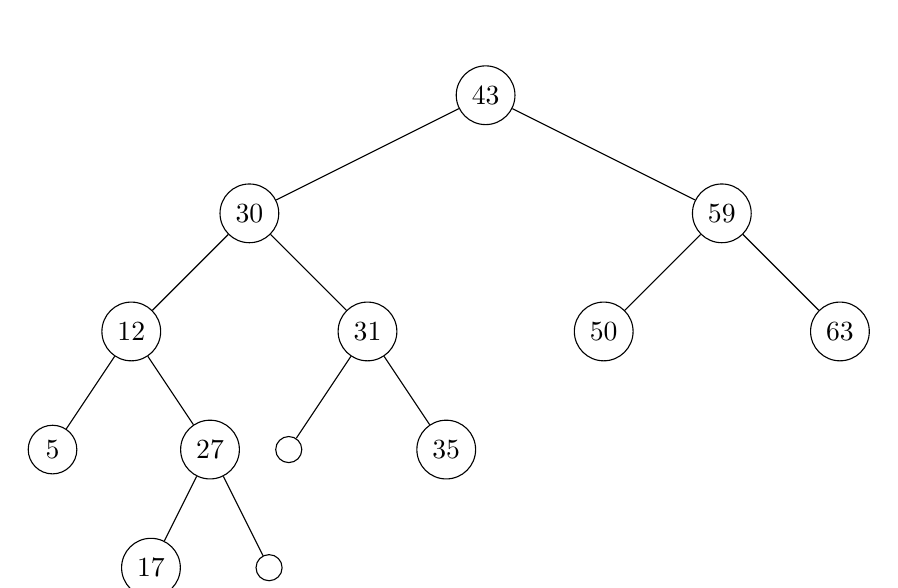
\begin{tikzpicture}[level/.style={sibling distance=60mm/#1}]
\node [circle,draw] (z){$43$}
  child {node [circle,draw] (a) {$30$}
    child {node [circle,draw] (b) {$12$}
       child {node [circle,draw] (c) {$5$}}
       child {node [circle,draw] (d) {$27$}
          child {node [circle,draw] (e) {$17$}}
          child {node [circle,draw] (l) {}}
       }
    }
    child {node [circle,draw] (f) {$31$}
       child {node [circle,draw] (m) {}}
       child {node [circle,draw] (g) {$35$}}
    }
  }
  child {node [circle,draw] (h) {$59$}
    child {node [circle,draw] (i) {$50$}}
    child {node [circle,draw] (k) {$63$}}
  };
\end{tikzpicture}}
\end{center}

Rotation 

\begin{center}
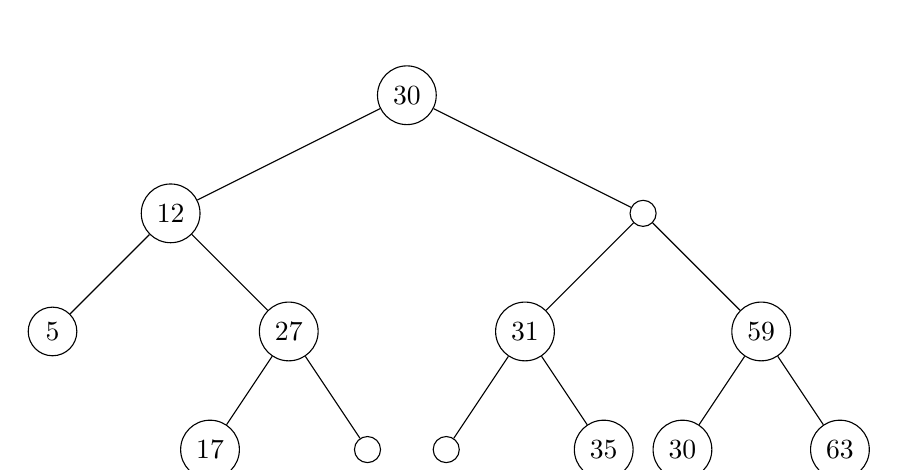
\begin{tikzpicture}[level/.style={sibling distance=60mm/#1}]
\node [circle,draw] (z){$30$}
  child {node [circle,draw] (a) {$12$}
    child {node [circle,draw] (b) {$5$}
    }
    child {node [circle,draw] (f) {$27$}
       child {node [circle,draw] (g) {$17$}}
       child {node [circle,draw] (n) {}}
    }
  }
  child {node [circle,draw] (h) {$ $}
    child {node [circle,draw] (i) {$31$}
       child {node [circle,draw] (o) {}}
       child {node [circle,draw] (j) {$35$}}
    }
    child {node [circle,draw] (k) {$59$}
       child {node [circle,draw] (l) {$30$}}
       child {node [circle,draw] (m) {$63$}}
    }
  };
\end{tikzpicture}}
\end{center}

nach 43 gelöscht

\begin{center}
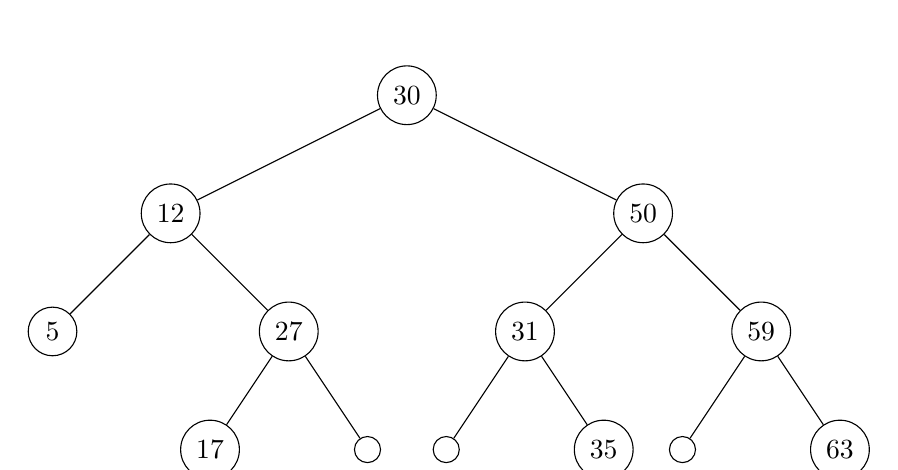
\begin{tikzpicture}[level/.style={sibling distance=60mm/#1}]
\node [circle,draw] (z){$30$}
  child {node [circle,draw] (a) {$12$}
    child {node [circle,draw] (b) {$5$}
    }
    child {node [circle,draw] (f) {$27$}
       child {node [circle,draw] (g) {$17$}}
       child {node [circle,draw] (l) {}}
    }
  }
  child {node [circle,draw] (h) {$50$}
    child {node [circle,draw] (i) {$31$}
       child {node [circle,draw] (n) {}}
       child {node [circle,draw] (j) {$35$}}
    }
    child {node [circle,draw] (k) {$59$}
       child {node [circle,draw] (o) {}}
       child {node [circle,draw] (m) {$63$}}
    }
  };
\end{tikzpicture}}
\end{center}

\paragraph{c)} 
Leiten Sie eine Eingabefolge von $n$ Zahlen für einen AVL-Baum ab, die keine Rotationen erfordert. \\

Nehme an die Eingabe ist oder wurde zuvor sortiert. Wähle nun als Einfüge-Element  den Median und teile die Eingabe in zwei weitere sortierte Eingaben. Wähle nun als Einfüge-Element zuerst den linken, dann den rechten Median. Nun gibt es vier Eingaben (sortiert) von denen wieder zuerst die Mediane bestimmt werden müssen und ausschließend nacheinander eingefügt werden.

Die Eingabefolge ergibt sich nur aus der Einfüge-Reihenfolge der Elemente der sortierten Eingabe: Sortiere eine sortierte Eingabefolge um, dass die Mediane der sortierten Teilfolge von links nach rechts aufgereiht werden. Falls die Eingabefolge keine eindeutigen Mediane hat, füge beide Median-Element hinzu.


%----------------------------------------------------------------------------
\subsection{Binäre Suchbäume}

\paragraph{a)}
 Gegeben ein Pfad $P$ von der Wurzel zum Blatt eines binären Suchbaumes. Sei $B$ die Menge der Knoten auf diesem Pfad,
$A$ alle Knoten links von $P$ und $C$ alle Knoten rechts von $P$. Gilt dann $a\le b\le c$ für alle $a\in A$, $b\in B$ und $c\in C$? \\

\textbf{Nein} Gegenbeispiel:

\begin{center}
\begin{tikzpicture}[level/.style={sibling distance=60mm/#1}]
\node [circle,draw] (z){$50$}
  child {node [circle,draw] (a) {$40$}}
  child {node [circle,draw] (g) {$60$}
    child {node [circle,draw] (h) {$55$}}
    child {node [circle,draw] (h) {$70$}
       child {node [circle,draw] (i) {}}
       child {node [circle,draw] (j) {$80$}}
    }
  };
\end{tikzpicture}}
\end{center}

ist binärer Suchbaum, weil $\forall$ Knoten n gilt:
\begin{itemize}
\item $childr(n) \geq n$
\item $childl(n) < n$
\end{itemize} \\

Wähle Pfad $P=(50,60,70,80)$ \\
$\Rightarrow A=(40,55); C = \emptyset$ \\
$|P|=4,|A|=2, |C| = 0$ \\
$|A| \leq |P| > |B| \neq |A| \leq |P| \leq C$ \\
$a \leq b \leq c$ mit $a \in A, b \in B, c \in C$ gilt nicht\\

\paragraph{b)} Zeigen Sie: Hat ein Knoten in einem binären Suchbaum zwei Kinder, so hat sein Nachfolger kein linkes Kind und sein Vorgänger kein rechtes Kind. Gilt diese Aussage auch für ein Knoten mit nur einem Kind? \\

Sei $x_{i} \in \mathbb{Z}$ und $x_{0} < x_{1} < ... < x_{n}$ \\

\textbf{Geg}: \begin{itemize}
\item $x_{i}$ 2 Kinder
\item $x_{i-1}$ Vorgänger von $x_{i}$
\item $x_{i+1}$ Nachfolger
\end{itemize} 

\textbf{Beh}: $x_{i-1}$ hat kein rechtes Kind, $x_{i+1}$ hat kein linkes Kind \\

\textbf{Bew} 
Da $x_{i-1}$ Vorgänger von $x_{i}$: \\

$\Rightarrow x_{i-1} < x_{i} \wedge \nexists x_{j} \in [x_{i-1};x_{i}]$ \\

Da nun $x_{i-1}$ nicht Kind von $x_{i}$ (weil $x_{i}$ schon 2 Kinder hat) sein kann, existiert kein $x_{j}$ zwischen $x_{i-1}$ und $x_{i}$ \\

$\Rightarrow x_{i-1}$ Vorgänger kann kein rechtes Kind $x_{j}$ mehr erhalten \\

Da $x_{i+1}$ Nachfolger von $x_{i}$: \\

$\Rightarrow x_{i+1} > x_{i} \wedge \nexists x_{j} \in [x_{i};x_{i+1}]$ \\

Da $x_{i}$ schon 2 Kinder hat \\

$\Rightarrow x_{i+1}$ Nachfolger kann kein rechtes Kind $x_{j}$ mehr erhalten \\

Diese Aussage gilt für Knoten mit nur einem Kind, aber nur falls Knoten bereits linkes Kind besitzt bei Vorgänger-Einfügung. Ebenso gilt die Aussage falls Knoten bereits rechtes Kind besitzt für den Nachfolger.

\paragraph{c)}Zeigen oder widerlegen Sie: Sei $T$ ein binärer Suchbaum und seien $x$ und $y$ Elemente in $T$. Der binäre Suchbaum, der sich nach Löschen von $x$ und $y$ (in dieser Reihenfolge) ergibt ist derselbe Suchbaum, der sich nach Löschen von $y$ und $x$ (in dieser Reihenfolge) ergibt. \\

T Bin. SB, $x,y \in binSB$ \\

Da beim Löschen immer das kleinste Element des rechte oder das größte des linken TB gewählt werden, wird immer ein Blatt für x oder y als Ersatz gewählt, welches anschließend gelöscht wird. Da sich dadurch die Reihenfolge innerhalb des Baumes dadruch nicht verändert kann in beliebiger Reihenfolge gelöscht werden.

%----------------------------------------------------------------------------
\subsection{Rot-Schwarz-Bäume}
Rot-Schwarz-Bäume sind eine Möglichkeit, um balancierte Suchbäume zu implementieren. Wir betrachten nun binäre Suchbäume, deren Knoten folgende Felder enthalten: {\em color, key, left, right} und {\em p} (Parent). Alle Knoten werden als innere Knoten betrachtet, die Blätter durch Zeiger auf \texttt{nil} dargestellt. 
Ein binärer Suchbaum, der folgende Eigenschaften erfüllt, ist ein Rot-Schwarz-Baum:
\begin{enumerate}
\item Jeder Knoten ist schwarz oder rot.
\item Die Wurzel ist schwarz.
\item Jedes Blatt (\texttt{nil}) ist schwarz.
\item Falls ein Knoten rot ist, so sind beide Kinder schwarz.
\item Für jeden Knoten gilt: Alle Pfade zu den Nachfahren, die Blätter (\texttt{nil}) sind, haben die gleiche Anzahl von schwarzen Knoten.
\end{enumerate}

\paragraph{a)} 
Färben Sie den angegebenen Suchbaum so, dass es sich um einen Rot-Schwarz-Baum handelt. \\

\begin{center}
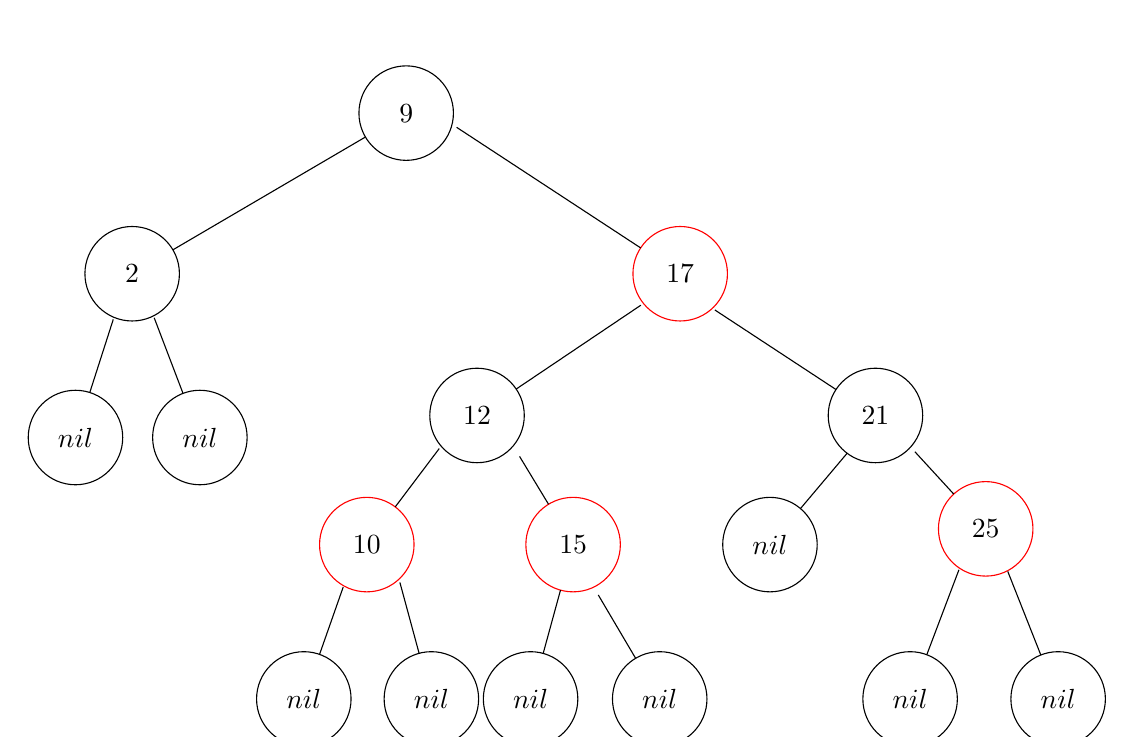
\begin{tikzpicture}[scale=0.2]
\tikzstyle{every node}+=[inner sep=0pt]
\draw [black] (33.4,-8.2) circle (3);
\draw (33.4,-8.2) node {$9$};
\draw [black] (16,-18.4) circle (3);
\draw (16,-18.4) node {$2$};
\draw [black] (12.4,-28.8) circle (3);
\draw (12.4,-28.8) node {$nil$};
\draw [black] (20.3,-28.8) circle (3);
\draw (20.3,-28.8) node {$nil$};
\draw [red] (50.8,-18.4) circle (3);
\draw (50.8,-18.4) node {$17$};
\draw [black] (37.9,-27.4) circle (3);
\draw (37.9,-27.4) node {$12$};
\draw [black] (63.2,-27.4) circle (3);
\draw (63.2,-27.4) node {$21$};
\draw [red] (30.9,-35.6) circle (3);
\draw (30.9,-35.6) node {$10$};
\draw [red] (44,-35.6) circle (3);
\draw (44,-35.6) node {$15$};
\draw [black] (56.5,-35.6) circle (3);
\draw (56.5,-35.6) node {$nil$};
\draw [red] (70.2,-34.6) circle (3);
\draw (70.2,-34.6) node {$25$};
\draw [black] (65.4,-45.4) circle (3);
\draw (65.4,-45.4) node {$nil$};
\draw [black] (74.8,-45.4) circle (3);
\draw (74.8,-45.4) node {$nil$};
\draw [black] (49.5,-45.4) circle (3);
\draw (49.5,-45.4) node {$nil$};
\draw [black] (41.3,-45.4) circle (3);
\draw (41.3,-45.4) node {$nil$};
\draw [black] (35,-45.4) circle (3);
\draw (35,-45.4) node {$nil$};
\draw [black] (26.9,-45.4) circle (3);
\draw (26.9,-45.4) node {$nil$};
\draw [black] (30.81,-9.72) -- (18.59,-16.88);
\draw [black] (14.8,-21.3) -- (13.31,-25.94);
\draw [black] (17.4,-21.2) -- (19.23,-26);
\draw [black] (36.6,-9.1) -- (48.29,-16.76);
\draw [black] (48.3,-20.4) -- (40.39,-25.72);
\draw [black] (53,-20.7) -- (60.69,-25.75);
\draw [black] (61.4,-29.8) -- (58.44,-33.31);
\draw [black] (65.7,-29.7) -- (68.17,-32.39);
\draw [black] (68.5,-37.2) -- (66.46,-42.59);
\draw [black] (71.6,-37.3) -- (73.7,-42.61);
\draw [black] (45.6,-38.8) -- (47.97,-42.82);
\draw [black] (43.2,-38.49) -- (42.1,-42.51);
\draw [black] (33,-38) -- (34.22,-42.5);
\draw [black] (29.4,-38.3) -- (27.9,-42.57);
\draw [black] (35.5,-29.5) -- (32.71,-33.2);
\draw [black] (40.6,-30) -- (42.44,-33.04);
\end{tikzpicture}
\end{center}

\paragraph{b)} 
In einem Rot-Schwarz-Baum ist das Einfügen von Elementen eine komplizierte Operation,
die eventuell Rebalancierungen und Umfärbungen nach sich zieht.
Fügen Sie zwei geeignete Elemente so in den Suchbaum ein, dass Ihre Färbung aus Teil (a)
erhalten bleibt und trotzdem ein gültiger Rot-Schwarz-Baum entstehen. \\

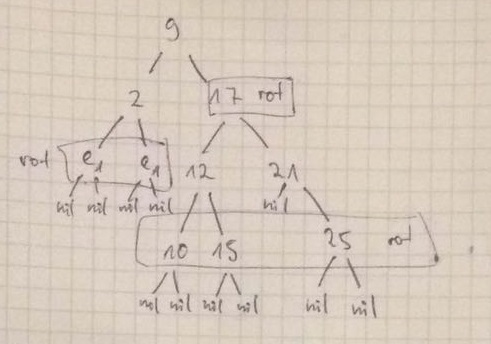
\includegraphics[width=10cm,height=5cm]{baum06A3b.jpg} \\

\paragraph{c)}
Zeigen Sie, dass ein Red-Black-Tree höchstens Tiefe $2\log(n+1)$ hat. Dabei ist
$n$ die Anzahl der (inneren) Knoten. \\

Da die Rot-Schwarz Bedingung des Baums zur halben Ausgeglichenheit zwingst wegen E.5(-E.1) (gleiche Anzahl schwarzer Knoten im Baum $\forall$ Pfade), gilt es bei fast voller Ausgeglichenheit $log(n+1)$ Tiefe (wegen der Wurzel die schwarz sein muss und keinen linken Teilbaum haben könnte.) Da nun aber jeder zweite Teilbaum aber lineare Liste werden kann, kann die doppelte Tiefe, also $2*log(n+1)$ erreicht werden.

\paragraph{d)} 
Ist jeder Rot-Schwarz-Baum auch ein AVL-Baum? Begründen Sie Ihre Antwort. \\

\textbf{Nein}
Gegenbeispiel siehe geg. Rot-Schwarz-Baum aus a)

%----------------------------------------------------------------------------
\subsection{Implementation von Binären Suchbäumen}
Laden Sie die Java-Vorlage aus dem Moodle herunter und implementieren Sie:

\paragraph{a)} 
Die Klasse \texttt{BSTreeNode}, die das gegebene Interface \texttt{TreeNode} implementiert.

\paragraph{b)} 
Die fünf Methoden der Klasse \texttt{BSTree}, die keine Implementierung haben.

%----------------------------------------------------------------------------------------
\newpage
\section{Blatt 07}
%----------------------------------------------------------------------------
\subsection{Anwendung von AVL-Bäumen}
Betrachten Sie folgendes Problem: Gegeben eine Menge $C$ von Kreisen:
\[ C = \{c_i = (x_i,y_i, r_i) \mid i = 1,\dots,n \}. \]
Dabei ist $(x_i,y_i)$ der Mittelpunkt und $r_i>0$ der Radius des Kreises $c_i$.
Sie können annehmen, dass sich keine drei Kreise in einem Punkt schneiden und dass es keinen Kreis gibt,
der vollkommen in einem anderen Kreis enthalten ist.
Gefragt ist nun nach dem \textit{Schnittproblem}, das heißt nach allen Schnittpunkten
der Kreise in $C$. Für Ihre Analyse dürfen Sie annehmen, dass die Schnittpunkte von
zwei Kreisen mit einer gegebenen Funktion \texttt{Schnitt($c_i$,$c_j$)} in Zeit $O(1)$ berechnet werden können.
Geben Sie einen \textit{Plane-Sweep} Algorithmus für das Schnittproblem in Pseudocode an.
Halten Sie sich dabei an folgende Hilfestellungen: Verwenden Sie eine $X$-Struktur
und eine $Y$-Struktur (beides AVL-Bäume), die ,,wichtige'' $x$- und $y$-Werte enthalten.
Geben Sie die Laufzeit Ihres Algorithmus an und begründen Sie die Korrektheit Ihres Algorithmus. \\

\begin{algorithm}[H]
\SetAlgoLined
\textbf{Data} C (Menge von Kreisen)  \\
\textbf{Result} gesamte Anzahl an Schnittpunkten der Kreise \\
Sei A und B ein leerer AVL-Baum \\
Sei v und w eine leere Liste \\
Sortiere C nach x-Werten (x-Werte: $x=x_{i}-r_{i}$) \\
\textbf{for} alle Kreise $c_{i}$ \textbf{do} \\
 | Berechne linkesten und rechtesten x-Wert von $c_{i}$ \\
 | Füge x-Werte nach ihren Werten in A ein \\
 | Berechne obersten und untersten y-Wert von $c_{i}$ \\
 | Füge y-Werte nach ihren Werten in B ein \\
\textbf{end} \\
v $\leftarrow$ InterceptionFinder(C,A,B) \\
\textbf{for} alle Verbindungen von Kreisen in v \textbf{do} \\
 | Schnitt$(c_{i},c_{j})$ schreibe in w \\
\textbf{end} \\
\textbf{return} w 
\end{algorithm} \\

\textbf{InterceptionFinder} 
\begin{algorithm}[H]
\SetAlgoLined
\textbf{Data} C (Menge von Kreisen), A und B (AVL-Bäume) \\
\textbf{Result} eine Liste R aller Verbindungen der Kreise \\
\textbf{for} jedes $c_{i}$ in C \textbf{do} \\
 | Suche linkeste und rechteste x-Wert in A \\
 | Suche oberste und unterste y-Wert in B \\
 | überprüfe alle Kanten von den vier Punkten \\
\textbf{if} Kanten der Punkte in A und B die selben Kreise verbinden \\
 | schreiben Verbindung in Liste v \\
\textbf{end}\\
\textbf{end}  
\end{algorithm} \\

n gibt Die Anzahl der Kreise in C an. Der Algorithmus sortiert einmal die Menge der Kreise nach dem am linkesten liegendem x-Wert mit einer Laufzeit von $O(n*log(n))$. Dann durchläuft er die Liste von links nach rechts und bestimmt für jeden Kreis vier Werte: die äußersten liegenden Werte (linkeste, rechteste,oberste, unterste) mit $O(4*n) \Rightarrow O(n)$. Die Werte werden dann in die AVL-Bäume eingetragen (worst case: $O (log(n))$). Danach wird unser 2.Algorithmus der InterceptionFinder aufgerufen: er findet Kantenverbindungen der Knoten im Baum eines Kreises zu den Knoten der anderen Kreise. Er speichert sie in einer Liste nur, wenn sie in beiden AVL-Bäume vorkommen. D.h. ein Kreis gilt als geschnitten, wenn einer der x-Werte des ersten Kreises mit einem der x-Werte des zweiten Kreises eine gemeinsame Kante besitzen und dasselbe muss auch für einen y-Wert gelten. Also hat man mit einer linearen Suche, weil die Liste unsortiert ist eine Laufzeit von $O(n)$. Das Finden der Kanten läuft hingegen in konstanter Zeit $O(1)$. Um die Liste aller Verbindungen aufzurufen, wird wieder eine konstante Laufzeit für das Problem gelöst. (Worst case: $O(n)$). \\

Damit beträgt die Laufzeit: \\
$O (n*log(n))+O (n)+O (log(n))+O (n)+O (1)+O} (n)=O (n*log(n))$

\subsubsection{Korrektur}

\textbf{in X-Structure we save events ordered by x-value}
\begin{itemize}
\item start of circle
\item end of cirlce
\item intersections of different circles
\end{itemize} \\

\textbf{in Y-Structure we save semi-circles ordered by y-value}
\begin{itemize}
\item start of circle
divide the circle into two semi-circles $c_{l}$ and $c_{u}$ \\
insert both into Y-structure \\
determine the intersections with predecessor and successor in Y-structure \\
insert new intersection-events into X-structure 
\item end of circle
determine intersections of predecessor and successor of current circle \\
new intersection-events into X-structure \\
delete the current circle in the Y-structure
\item intersection of different circles
save intersections \\
suppose two semi-circles $c_{i}$ and $c_{j}$ are intersecting, where $c_{j}$ is successor of $c_{i}$ \\
determine intersections \\
switch $c_{i}$ and $c_{j}$ in the Y-structure
\end{itemize}

\textbf{intersections(C)} 
\begin{algorithm}[H]
\SetAlgoLined
initialize list P \\
fill X-Structure with start and end points of all circles \\
\While{X not empty} {
  get and remove first event e in X \;
  \eIF{e is start of circle} {
  create lower circle $c_{l}$ and upper circle $c_{u}$ from current circle \;
  insert $c_{l}$ and $c_{u}$ into Y-strcture \;
  determine intersections of $c_{l}$ with its predecessor in Y-structure \;
  add intersections events to X \;
  determine intersections of $c_{r}$ with ist successor in Y-structure \;
  add intersection events to X \;
  } {
     \eIF{e is end of circle} {
     let c be current circle \;
     determine intersections of predecessor $c_{l}$ with successor $c_{u}$ \;
     insert new intersection evens to X \;
     delete current circle from Y-structure \;
     }{
     e is intersection of different circles \;
     add the new intersection to P \;
     let $c_{i}$ and $c_{j}$ = successor $c_{i}$ be the corresponding crossing semi-sircles \;
     determine intersections of $c_{i}$ with successor $c_{j}$ \;
     add new intersection events to X \;
     switch $c_{i}$ and $c_{j}$ in Y-structure \;
     }
}
\textbf{return} P;
\end{algorithm} \\

%----------------------------------------------------------------------------
\subsection{B-Bäume}
In dieser Aufgabe geht es um B-Bäume der Ordnung 2, d.\,h. ein innerer Knoten hat mindestens zwei und höchstens drei Kinder. Gegeben ist der folgende B-Baum der Ordnung 2:


\paragraph{a)}
Fügen Sie die folgenden Elemente in den gegebenen B-Baum ein: Zuerst 14 und dann 1. \\

\begin{center}
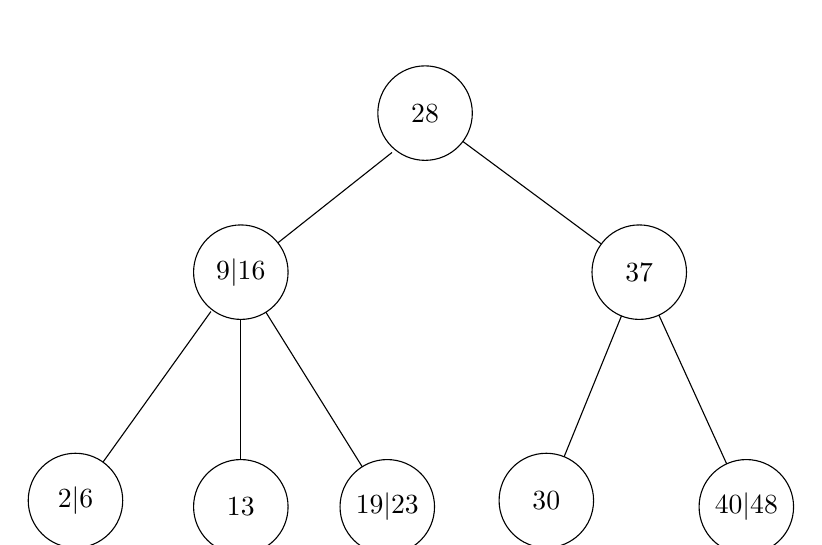
\begin{tikzpicture}[scale=0.2]
\tikzstyle{every node}+=[inner sep=0pt]
\draw [black] (38.1,-14.1) circle (3);
\draw (38.1,-14.1) node {$28$};
\draw [black] (26.4,-24.2) circle (3);
\draw (26.4,-24.2) node {$9|16$};
\draw [black] (51.7,-24.2) circle (3);
\draw (51.7,-24.2) node {$37$};
\draw [black] (15.9,-38.7) circle (3);
\draw (15.9,-38.7) node {$2|6$};
\draw [black] (26.4,-39.1) circle (3);
\draw (26.4,-39.1) node {$13$};
\draw [black] (35.7,-39.1) circle (3);
\draw (35.7,-39.1) node {$19|23$};
\draw [black] (58.5,-39.1) circle (3);
\draw (58.5,-39.1) node {$40|48$};
\draw [black] (45.8,-38.7) circle (3);
\draw (45.8,-38.7) node {$30$};
\draw [black] (52.95,-26.93) -- (57.25,-36.37);
\draw [black] (40.5,-15.9) -- (49.29,-22.41);
\draw [black] (50.57,-26.98) -- (46.93,-35.92);
\draw [black] (36,-16.6) -- (28.75,-22.34);
\draw [black] (27.99,-26.74) -- (34.11,-36.56);
\draw [black] (26.4,-27.2) -- (26.4,-36.1);
\draw [black] (24.5,-26.7) -- (17.65,-36.26);
\end{tikzpicture}
\end{center}

14 einfügen \\

\begin{center}
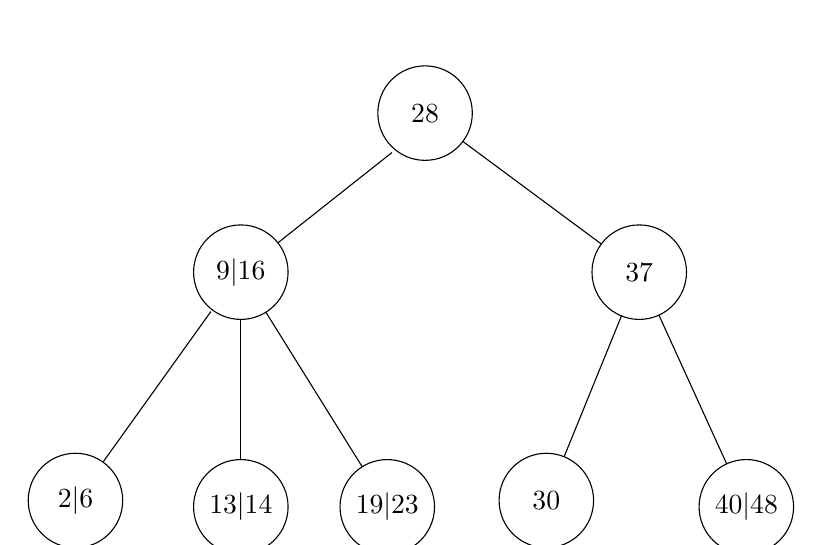
\begin{tikzpicture}[scale=0.2]
\tikzstyle{every node}+=[inner sep=0pt]
\draw [black] (38.1,-14.1) circle (3);
\draw (38.1,-14.1) node {$28$};
\draw [black] (26.4,-24.2) circle (3);
\draw (26.4,-24.2) node {$9|16$};
\draw [black] (51.7,-24.2) circle (3);
\draw (51.7,-24.2) node {$37$};
\draw [black] (15.9,-38.7) circle (3);
\draw (15.9,-38.7) node {$2|6$};
\draw [black] (26.4,-39.1) circle (3);
\draw (26.4,-39.1) node {$13|14$};
\draw [black] (35.7,-39.1) circle (3);
\draw (35.7,-39.1) node {$19|23$};
\draw [black] (58.5,-39.1) circle (3);
\draw (58.5,-39.1) node {$40|48$};
\draw [black] (45.8,-38.7) circle (3);
\draw (45.8,-38.7) node {$30$};
\draw [black] (52.95,-26.93) -- (57.25,-36.37);
\draw [black] (40.5,-15.9) -- (49.29,-22.41);
\draw [black] (50.57,-26.98) -- (46.93,-35.92);
\draw [black] (36,-16.6) -- (28.75,-22.34);
\draw [black] (27.99,-26.74) -- (34.11,-36.56);
\draw [black] (26.4,-27.2) -- (26.4,-36.1);
\draw [black] (24.5,-26.7) -- (17.65,-36.26);
\end{tikzpicture}
\end{center}

1 einfügen \\

\begin{center}
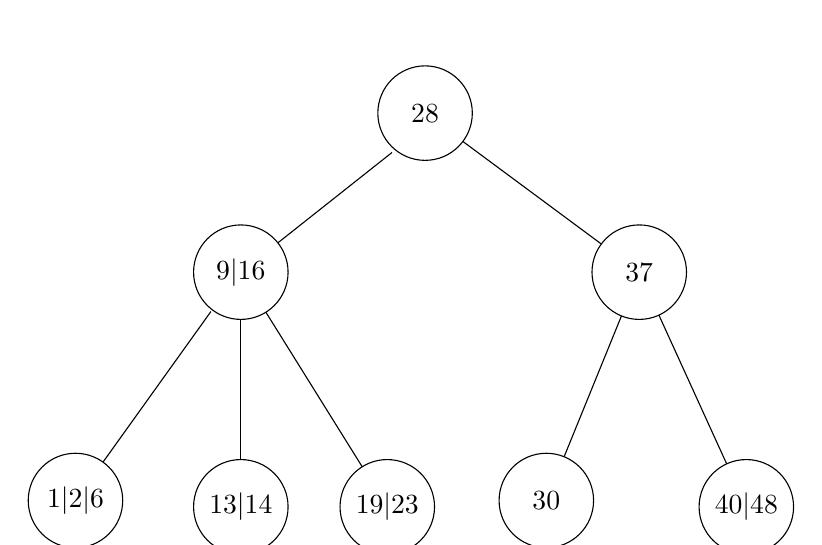
\begin{tikzpicture}[scale=0.2]
\tikzstyle{every node}+=[inner sep=0pt]
\draw [black] (38.1,-14.1) circle (3);
\draw (38.1,-14.1) node {$28$};
\draw [black] (26.4,-24.2) circle (3);
\draw (26.4,-24.2) node {$9|16$};
\draw [black] (51.7,-24.2) circle (3);
\draw (51.7,-24.2) node {$37$};
\draw [black] (15.9,-38.7) circle (3);
\draw (15.9,-38.7) node {$1|2|6$};
\draw [black] (26.4,-39.1) circle (3);
\draw (26.4,-39.1) node {$13|14$};
\draw [black] (35.7,-39.1) circle (3);
\draw (35.7,-39.1) node {$19|23$};
\draw [black] (58.5,-39.1) circle (3);
\draw (58.5,-39.1) node {$40|48$};
\draw [black] (45.8,-38.7) circle (3);
\draw (45.8,-38.7) node {$30$};
\draw [black] (52.95,-26.93) -- (57.25,-36.37);
\draw [black] (40.5,-15.9) -- (49.29,-22.41);
\draw [black] (50.57,-26.98) -- (46.93,-35.92);
\draw [black] (36,-16.6) -- (28.75,-22.34);
\draw [black] (27.99,-26.74) -- (34.11,-36.56);
\draw [black] (26.4,-27.2) -- (26.4,-36.1);
\draw [black] (24.5,-26.7) -- (17.65,-36.26);
\end{tikzpicture}
\end{center}

Knoten $(1|2|6)$ hat zu viele Elemente $\rightarrow$ Ordnung 2 nicht mehr erfüllt \\

teile den Knoten $(1|2|6)$  und lasse die 2 nach oben steigen \\

Knoten $(2|9|16)$ hat dann wiederum auch zu viele Elemente \\
$\rightarrow$ aufspalten und 9 nach oben wandern \\

\begin{center}
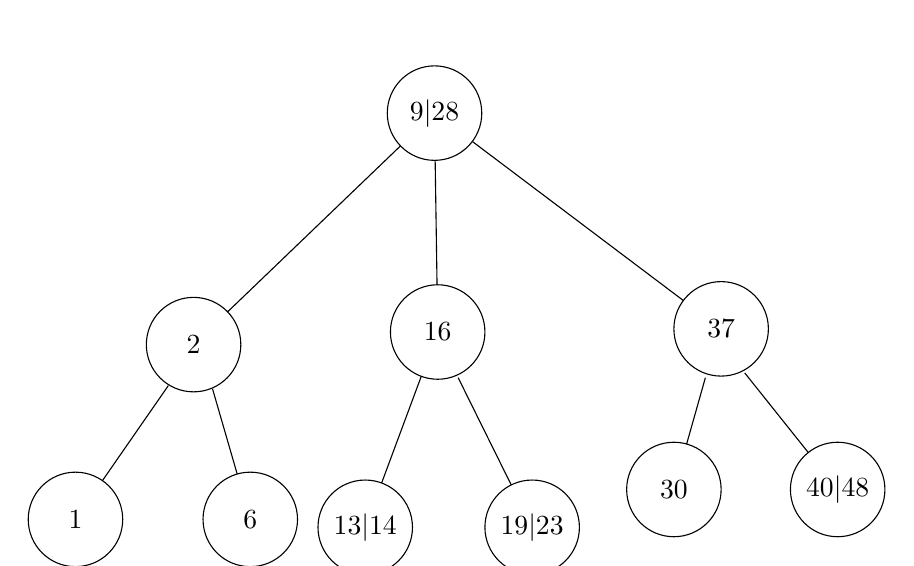
\begin{tikzpicture}[scale=0.2]
\tikzstyle{every node}+=[inner sep=0pt]
\draw [black] (39.4,-14.3) circle (3);
\draw (39.4,-14.3) node {$9|28$};
\draw [black] (39.6,-28.2) circle (3);
\draw (39.6,-28.2) node {$16$};
\draw [black] (24.1,-29) circle (3);
\draw (24.1,-29) node {$2$};
\draw [black] (57.6,-28) circle (3);
\draw (57.6,-28) node {$37$};
\draw [black] (16.6,-40.1) circle (3);
\draw (16.6,-40.1) node {$1$};
\draw [black] (27.7,-40.1) circle (3);
\draw (27.7,-40.1) node {$6$};
\draw [black] (35,-40.6) circle (3);
\draw (35,-40.6) node {$13|14$};
\draw [black] (45.6,-40.6) circle (3);
\draw (45.6,-40.6) node {$19|23$};
\draw [black] (54.6,-38.2) circle (3);
\draw (54.6,-38.2) node {$30$};
\draw [black] (65,-38.2) circle (3);
\draw (65,-38.2) node {$40|48$};
\draw [black] (37.24,-16.38) -- (26.26,-26.92);
\draw [black] (39.44,-17.3) -- (39.56,-25.2);
\draw [black] (41.8,-16.1) -- (55.2,-26.2);
\draw [black] (22.5,-31.6) -- (18.31,-37.64);
\draw [black] (25.3,-31.8) -- (26.87,-37.22);
\draw [black] (38.56,-31.01) -- (36.04,-37.79);
\draw [black] (40.9,-31.1) -- (44.27,-37.91);
\draw [black] (56.6,-31.1) -- (55.41,-35.31);
\draw [black] (59.1,-30.8) -- (63.13,-35.85);
\end{tikzpicture}
\end{center}

\paragraph{b)}
Löschen Sie die folgenden Elemente aus dem B-Baum, den Sie in Teil (a) erhalten haben: 37, 40, 19, 23 (in dieser Reihenfolge).  \\

Baum aus a) \\

\begin{center}
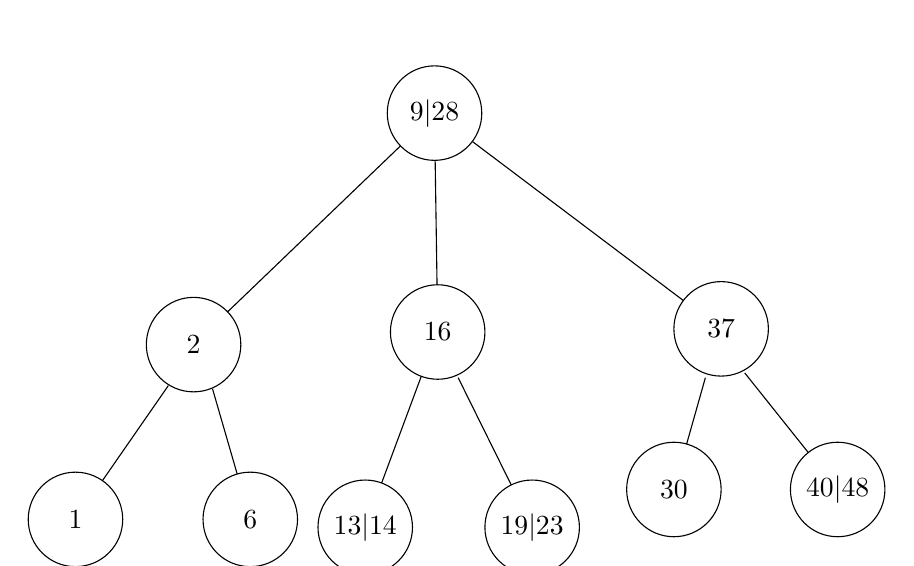
\begin{tikzpicture}[scale=0.2]
\tikzstyle{every node}+=[inner sep=0pt]
\draw [black] (39.4,-14.3) circle (3);
\draw (39.4,-14.3) node {$9|28$};
\draw [black] (39.6,-28.2) circle (3);
\draw (39.6,-28.2) node {$16$};
\draw [black] (24.1,-29) circle (3);
\draw (24.1,-29) node {$2$};
\draw [black] (57.6,-28) circle (3);
\draw (57.6,-28) node {$37$};
\draw [black] (16.6,-40.1) circle (3);
\draw (16.6,-40.1) node {$1$};
\draw [black] (27.7,-40.1) circle (3);
\draw (27.7,-40.1) node {$6$};
\draw [black] (35,-40.6) circle (3);
\draw (35,-40.6) node {$13|14$};
\draw [black] (45.6,-40.6) circle (3);
\draw (45.6,-40.6) node {$19|23$};
\draw [black] (54.6,-38.2) circle (3);
\draw (54.6,-38.2) node {$30$};
\draw [black] (65,-38.2) circle (3);
\draw (65,-38.2) node {$40|48$};
\draw [black] (37.24,-16.38) -- (26.26,-26.92);
\draw [black] (39.44,-17.3) -- (39.56,-25.2);
\draw [black] (41.8,-16.1) -- (55.2,-26.2);
\draw [black] (22.5,-31.6) -- (18.31,-37.64);
\draw [black] (25.3,-31.8) -- (26.87,-37.22);
\draw [black] (38.56,-31.01) -- (36.04,-37.79);
\draw [black] (40.9,-31.1) -- (44.27,-37.91);
\draw [black] (56.6,-31.1) -- (55.41,-35.31);
\draw [black] (59.1,-30.8) -- (63.13,-35.85);
\end{tikzpicture}
\end{center}

\textbf{lösche 37} und nehme 40 als Ersatzknoten \\

\begin{center}
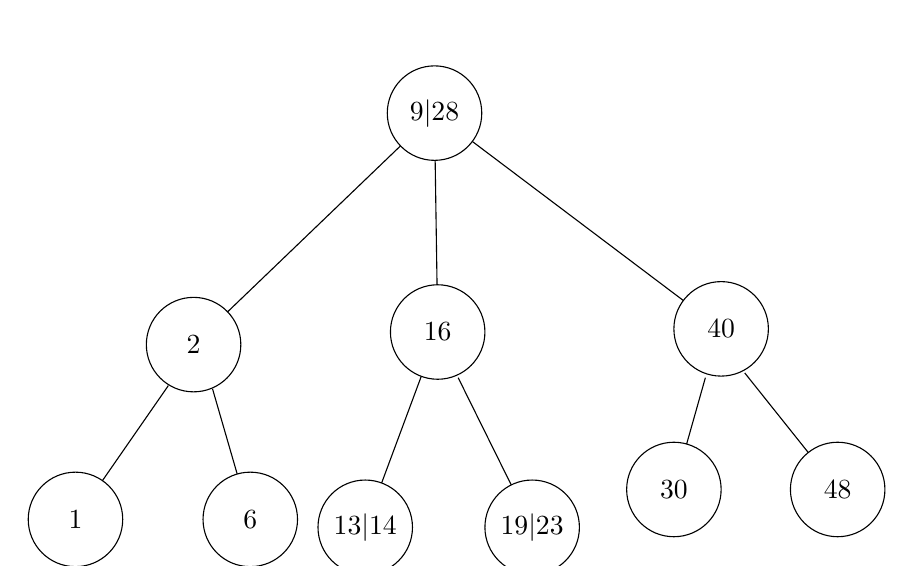
\begin{tikzpicture}[scale=0.2]
\tikzstyle{every node}+=[inner sep=0pt]
\draw [black] (39.4,-14.3) circle (3);
\draw (39.4,-14.3) node {$9|28$};
\draw [black] (39.6,-28.2) circle (3);
\draw (39.6,-28.2) node {$16$};
\draw [black] (24.1,-29) circle (3);
\draw (24.1,-29) node {$2$};
\draw [black] (57.6,-28) circle (3);
\draw (57.6,-28) node {$40$};
\draw [black] (16.6,-40.1) circle (3);
\draw (16.6,-40.1) node {$1$};
\draw [black] (27.7,-40.1) circle (3);
\draw (27.7,-40.1) node {$6$};
\draw [black] (35,-40.6) circle (3);
\draw (35,-40.6) node {$13|14$};
\draw [black] (45.6,-40.6) circle (3);
\draw (45.6,-40.6) node {$19|23$};
\draw [black] (54.6,-38.2) circle (3);
\draw (54.6,-38.2) node {$30$};
\draw [black] (65,-38.2) circle (3);
\draw (65,-38.2) node {$48$};
\draw [black] (37.24,-16.38) -- (26.26,-26.92);
\draw [black] (39.44,-17.3) -- (39.56,-25.2);
\draw [black] (41.8,-16.1) -- (55.2,-26.2);
\draw [black] (22.5,-31.6) -- (18.31,-37.64);
\draw [black] (25.3,-31.8) -- (26.87,-37.22);
\draw [black] (38.56,-31.01) -- (36.04,-37.79);
\draw [black] (40.9,-31.1) -- (44.27,-37.91);
\draw [black] (56.6,-31.1) -- (55.41,-35.31);
\draw [black] (59.1,-30.8) -- (63.13,-35.85);
\end{tikzpicture}
\end{center}

\textbf{lösche 40}:
30 oder 48 kann man nicht als Ersatzknoten wählen, da sonst die B-Baum Bedingungen nicht mehr erfüllt werden, d.h. verschmelze also $(30|48)$ zu einem Knoten und suche nach einem Vaterersatz: 28. Dieser sinkt ein Knoten nach unten und verschmilzt mit dem Knoten 16. \\

\begin{center}
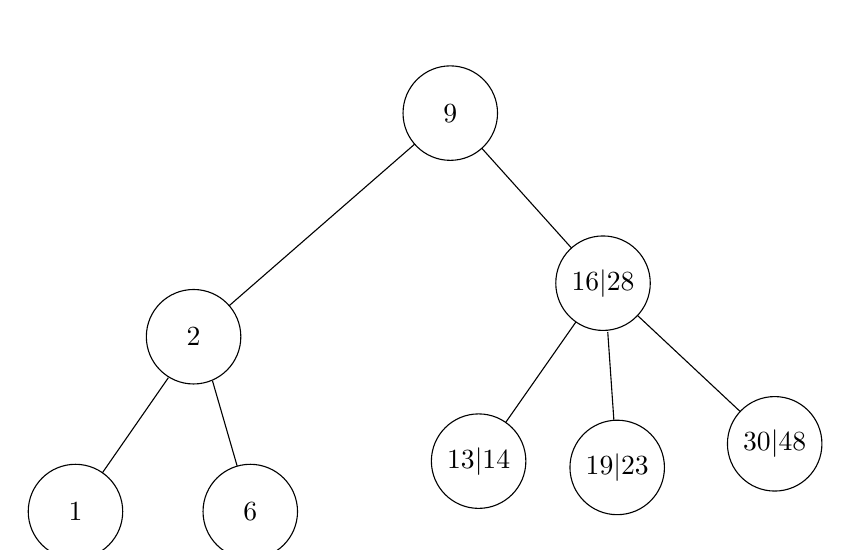
\begin{tikzpicture}[scale=0.2]
\tikzstyle{every node}+=[inner sep=0pt]
\draw [black] (24.1,-29) circle (3);
\draw (24.1,-29) node {$2$};
\draw [black] (16.6,-40.1) circle (3);
\draw (16.6,-40.1) node {$1$};
\draw [black] (27.7,-40.1) circle (3);
\draw (27.7,-40.1) node {$6$};
\draw [black] (40.4,-14.8) circle (3);
\draw (40.4,-14.8) node {$9$};
\draw [black] (50.1,-25.6) circle (3);
\draw (50.1,-25.6) node {$16|28$};
\draw [black] (42.2,-36.9) circle (3);
\draw (42.2,-36.9) node {$13|14$};
\draw [black] (51,-37.3) circle (3);
\draw (51,-37.3) node {$19|23$};
\draw [black] (61,-35.8) circle (3);
\draw (61,-35.8) node {$30|48$};
\draw [black] (22.5,-31.6) -- (18.31,-37.64);
\draw [black] (25.3,-31.8) -- (26.87,-37.22);
\draw [black] (38.14,-16.77) -- (26.36,-27.03);
\draw [black] (42.4,-17.03) -- (48.1,-23.37);
\draw [black] (48.38,-28.06) -- (43.92,-34.44);
\draw [black] (50.4,-28.7) -- (50.79,-34.31);
\draw [black] (52.29,-27.65) -- (58.81,-33.75);
\end{tikzpicture}
\end{center}

\textbf{lösche 19} \\

\begin{center}
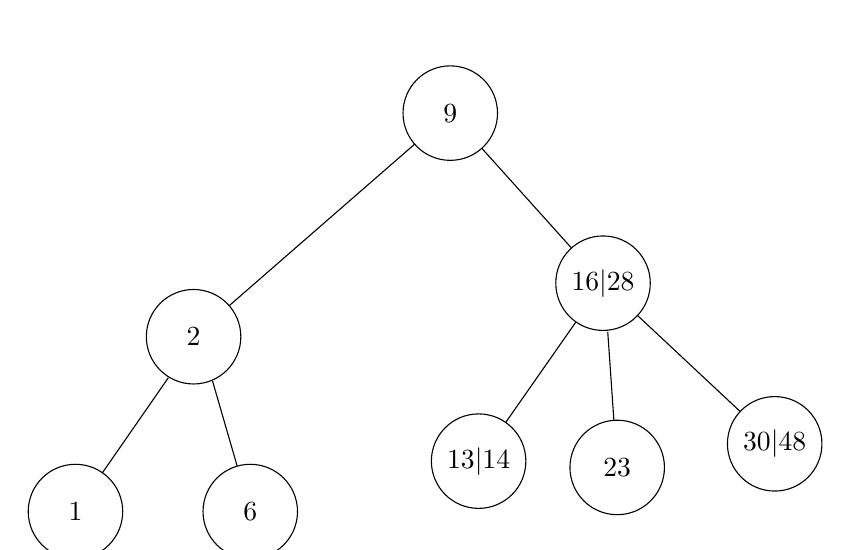
\begin{tikzpicture}[scale=0.2]
\tikzstyle{every node}+=[inner sep=0pt]
\draw [black] (24.1,-29) circle (3);
\draw (24.1,-29) node {$2$};
\draw [black] (16.6,-40.1) circle (3);
\draw (16.6,-40.1) node {$1$};
\draw [black] (27.7,-40.1) circle (3);
\draw (27.7,-40.1) node {$6$};
\draw [black] (40.4,-14.8) circle (3);
\draw (40.4,-14.8) node {$9$};
\draw [black] (50.1,-25.6) circle (3);
\draw (50.1,-25.6) node {$16|28$};
\draw [black] (42.2,-36.9) circle (3);
\draw (42.2,-36.9) node {$13|14$};
\draw [black] (51,-37.3) circle (3);
\draw (51,-37.3) node {$23$};
\draw [black] (61,-35.8) circle (3);
\draw (61,-35.8) node {$30|48$};
\draw [black] (22.5,-31.6) -- (18.31,-37.64);
\draw [black] (25.3,-31.8) -- (26.87,-37.22);
\draw [black] (38.14,-16.77) -- (26.36,-27.03);
\draw [black] (42.4,-17.03) -- (48.1,-23.37);
\draw [black] (48.38,-28.06) -- (43.92,-34.44);
\draw [black] (50.4,-28.7) -- (50.79,-34.31);
\draw [black] (52.29,-27.65) -- (58.81,-33.75);
\end{tikzpicture}
\end{center}

\textbf{lösche 23}:
Wenn man den Knoten 23 löscht, dann würde dem Knoten $(16|28)$ ein Kind fehlen, d.h. wir löschen 23 lassen 28 nach unten wandern und 30 nach oben. \\

\begin{center}
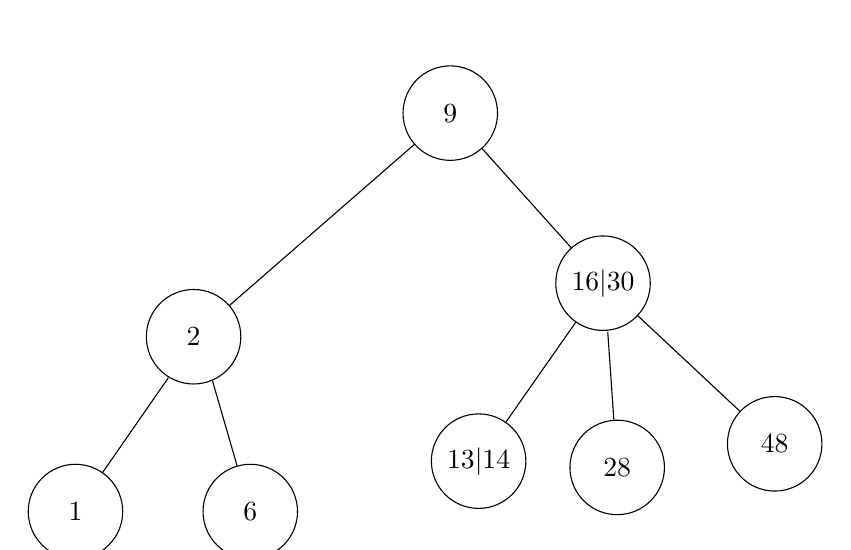
\begin{tikzpicture}[scale=0.2]
\tikzstyle{every node}+=[inner sep=0pt]
\draw [black] (24.1,-29) circle (3);
\draw (24.1,-29) node {$2$};
\draw [black] (16.6,-40.1) circle (3);
\draw (16.6,-40.1) node {$1$};
\draw [black] (27.7,-40.1) circle (3);
\draw (27.7,-40.1) node {$6$};
\draw [black] (40.4,-14.8) circle (3);
\draw (40.4,-14.8) node {$9$};
\draw [black] (50.1,-25.6) circle (3);
\draw (50.1,-25.6) node {$16|30$};
\draw [black] (42.2,-36.9) circle (3);
\draw (42.2,-36.9) node {$13|14$};
\draw [black] (51,-37.3) circle (3);
\draw (51,-37.3) node {$28$};
\draw [black] (61,-35.8) circle (3);
\draw (61,-35.8) node {$48$};
\draw [black] (22.5,-31.6) -- (18.31,-37.64);
\draw [black] (25.3,-31.8) -- (26.87,-37.22);
\draw [black] (38.14,-16.77) -- (26.36,-27.03);
\draw [black] (42.4,-17.03) -- (48.1,-23.37);
\draw [black] (48.38,-28.06) -- (43.92,-34.44);
\draw [black] (50.4,-28.7) -- (50.79,-34.31);
\draw [black] (52.29,-27.65) -- (58.81,-33.75);
\end{tikzpicture}
\end{center}

%----------------------------------------------------------------------------
\subsection{(2,4)-Bäume}
Begründen Sie jeweils die Korrektheit und Laufzeit Ihres Algorithmus.

\paragraph{a)} 
Seien $S$ und $T$ zwei (2,4)-Bäume, wobei alle Elemente aus $S$ kleiner sind
als die Elemente aus $T$, d.h. $\max S < \min T$.
Geben Sie einen effizienten Pseudocode-Algorithmus \texttt{merge($S,T$)} an,
der einen (2,4)-Baum aus der Vereinigung von $S$ und $T$ erstellt. \\

\textbf{merge(S,T)} \\
\begin{algorithm}[H]
\SetAlgoLined
m $\leftarrow$ biggest element in tree S \\
\eIF{height(S) $\leq$ height(T)} {
   T' $\leftarrow$ T \;
   \While{height(S) $\neq$ height(T')} {
   T' $\leftarrow$ leftmost child of root(T') \;
   }
   merge root(S) \;
   m and v= root(T') \;
   split tree T starting from v \;
   \textbf{return} T \;
} {
   S' $\leftarrow$ S \;
   \While {height(S') $\neq$ height(T)} {
   S' $\leftarrow$ rightmost child of root(S') \;
   }
   merge root(T) \;
   m and u=root(S') \;
   split the tree S starting from u \;
   \textbf{return} S \;
}
\end{algorithm}

\paragraph{b)}
Geben Sie einen effizienten Pseudocode-Algorithmus \texttt{split($T,x$)} an, 
der einen (2,4)-Baum $T$ am Wert $x$ in zwei (2,4)-Bäume $T_{\le x}$ und $T_{> x}$ aufspaltet. 
Dabei soll $T_{\le x}$ alle Elemente aus $T$ enthalten,
die kleiner oder gleich $x$ sind und $T_{> x}$ alle Elemente aus $T$, die größer als $x$ sind. \\

\textbf{split(S,x):} \\
\begin{algorithm}[H]
\SetAlgoLined
l,r $\leftarrow$ empty list \\
w $\leftarrow$ root(T)
\While {w is not leaf}{
   i $\leftarrow$ 1 \;
   \While {$i $} {
   }
}
\end{algorithm}

%----------------------------------------------------------------------------
\subsection{Amortisierte Analyse}
Eine \emph{Queue} ist eine Datenstruktur, die die beiden Operationen \texttt{enqueue} und \texttt{dequeue} unterstützt:
%
\begin{itemize}
\item \texttt{enqueue} zum Hinzufügen eines Objekts und
\item \texttt{dequeue} zum Zurückholen und Entfernen eines Objektes.
\end{itemize}

\noindent Dabei wird nach dem Prinzip \emph{first-in-first-out} gearbeitet, das heißt, es wird von \texttt{dequeue} immer das Objekt aus der Queue zurückgegeben, welches von den in der Queue noch vorhandenen Objekten als erstes mit \texttt{enqueue} hineingelegt wurde. 

\smallskip
\noindent
Ein \emph{Stack} ist eine Datenstruktur, die die drei Operationen
\texttt{push}, \texttt{pop} und \texttt{empty} unterstützt:
%
\begin{itemize}
\item \texttt{push} zum Hinzufügen eines Objekts,
\item \texttt{pop} zum Zurückholen und Entfernen eines Objektes, und
\item \texttt{empty} zum Prüfen, ob der Stack leer ist.
\end{itemize}

\noindent Dabei wird nach dem Prinzip \emph{last-in-first-out} gearbeitet, das heißt, es wird von \texttt{pop} immer das Objekt aus dem Stack zurückgegeben, welches von den in dem Stack noch vorhandenen Objekten als letztes mit \texttt{push} hineingelegt wurde. 

\paragraph{a)} 
Beschreiben Sie, wie man eine Queue mit Hilfe von zwei Stacks simulieren kann. \\

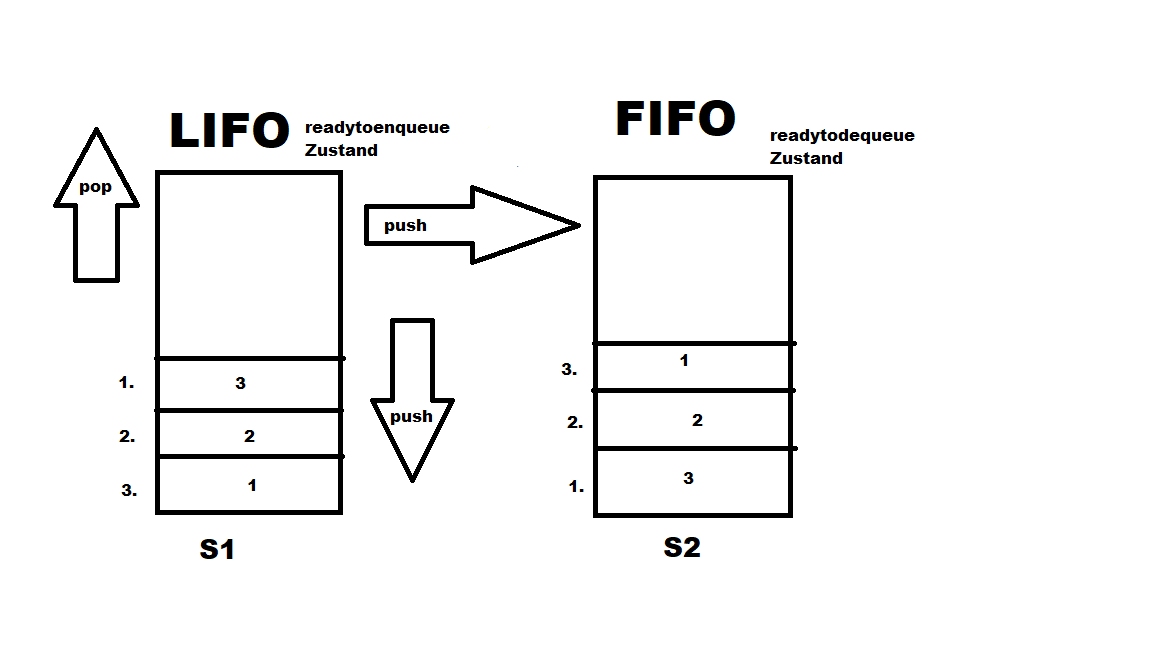
\includegraphics[width=15cm,height=10cm]{QueueStack.png} \\

Es gibt 2 Zustände für die Stacks: 
\begin{itemize}
\item readytoenqueue, wenn S2 leer ist
\item readytodequeue, wenn S1 leer ist
\end{itemize}

Hierbei wird in S1 die Reihenfolge für das Hinzufügen festgelegt und S2 muss hierfür leer sein. Soll dequeued werden, so gilt FIFO, also muss S1 und S2 gepusht werden, falls S2 zu Beginn dieser Operation leer war und anschließend stehen in S2 die Elemente aus S1 in verkehrter Reihenfolge, so dass man im readytodequeue Zustand landet und beliebig oft hintereinander FIFO ausgeben kann. Soll nun wieder enqueued werden, muss S2 wieder nach S1 gepushed werden, um in den readytoenqueue Zustand zu gelangen. \\

\textbf{enqueue(x):} \\
\begin{algorithm}[H]
\SetAlgoLined
\textbf{if} (not(empty(S1))): \\
\textbf{do} push(S2,S1) \\
enqueue(x)\\
\textbf{else} \\
\textbf{do} push(x,S1)
\end{algorithm}

\textbf{dequeue(x):} \\
\begin{algorithm}[H]
\SetAlgoLined
\textbf{if} (not(empty(S1))): \\
\textbf{do} push(S1,S2) \\
dequeue(x) \\
\textbf{else} \\
\textbf{do} pop(S2)
\end{algorithm}


\paragraph{b)} 
Zeigen Sie, dass die amortisierte Laufzeit für jede \texttt{enqueue}- und
\texttt{dequeue}-Operation von dieser simulierten Queue $O(1)$ ist. \\

\begin{tabular}{c|c|c|c}
& Einzahlung & Entsumme & Saldo/Ergebnis \\\hline
readytoqueue & kostet push(S2,S1) und $O(1)*n$ & $O(1)*n$ & push(S2,S1) \\\hline
readytodequeue & $O(1)*n$ & push(S1,S2) und $O(1)*n$ & push(S1,S2)
\end{tabular}

Da push$(s_{i},s_{j})$ n-Schritte für n Elemente benötigt ist die Laufzeit $O(1)$ \\
$\Rightarrow$ Saldo/Ergebnis der Account Methode der armortisiertes Laufzeitanalyse liegt in O(1).

%----------------------------------------------------------------------------------------
\newpage
\section{Tutorium 18.06.2018: Dynamisches Programmieren}

\textbf{Beispiel: Fibonacci}

\begin{algorithm}[H]
\SetAlgoLined
Fib(x) \\
fibarr[] = new Int[x] \\
fibarr[0]=0 \\
fibarr[1]=1 \\
\textbf{for}(i=2 to x) \\
      fibarr[i]=fibarr[i-1]+fibarr[i-2] \\
\textbf{return} fibarr[x]      
\end{algorithm}

%----------------------------------------------------------------------------------------
\newpage
\section{Blatt 08}
%----------------------------------------------------------------------------
\subsection{Skiplists}
Fügen Sie folgenden Elemente in eine Skiplist ein:
\[ 17,3,7,11,13,19,2,23,27. \]
Es stehen ihnen dazu folgende Zufallsbits zur Verfügung (von links nach rechts verbrauchen):
\[ 1101100101000110001. \]
Erhöhen Sie $L_i$ so lange bis das Zufallsbit $1$ ist. Geben Sie Ihre Datenstruktur nach jeder Ein\-füge\-operation an. \\

Bemerkung: Leider hat es uns zeitlich nicht gereicht, alle Querlinien einzufügen.  \\

\textbf{leere Skiplist} \\

\begin{tikzpicture}
\SetGraphUnit{1.5}
\SetVertexNormal[Shape    = rectangle,MinSize=.8 cm]
\Vertex[L=$-\infty$] {0;0}

\foreach \num/\label [count=\n from 0] in  
    {1/+\infty}
      {\EA[L=$\label$](\n;0){\num;0}} 
      
\foreach \num [remember=\num as \lastnum (initially 0)] in  {1}  
 {\Edge(\lastnum;0)(\num;0)}       
\end{tikzpicture} \\

\textbf{17,ZB:1} verbleibende ZB: 1011 0010 1000 1100 01 \\

\begin{tikzpicture}
\SetGraphUnit{1.5}
\SetVertexNormal[Shape    = rectangle,MinSize=.8 cm]
\Vertex[L=$-\infty$] {0;0}

\foreach \num/\label [count=\n from 0] in  
    {1/17 ,2/+\infty}
      {\EA[L=$\label$](\n;0){\num;0}} 
      
\foreach \num [remember=\num as \lastnum (initially 0)] in  {1,2}  
 {\Edge(\lastnum;0)(\num;0)}       
\end{tikzpicture} \\ 

\textbf{3, ZB:1} verbleibende ZB: 0110 0101 0001 1000 1 \\

\begin{tikzpicture}
\SetGraphUnit{1.5}
\SetVertexNormal[Shape    = rectangle,MinSize=.8 cm]
\Vertex[L=$-\infty$] {0;0}

\foreach \num/\label [count=\n from 0] in  
    {1/3, 2/17 ,3/+\infty}
      {\EA[L=$\label$](\n;0){\num;0}} 
      
\foreach \num [remember=\num as \lastnum (initially 0)] in  {1,2,3}  
 {\Edge(\lastnum;0)(\num;0)}       
\end{tikzpicture} \\ 


\textbf{7, ZB:01} $\rightarrow$ Levelerhöhung um 1; ZB: 1001 0100 0110 001 \\

\begin{tikzpicture}
\SetGraphUnit{1.5}
\SetVertexNormal[Shape    = rectangle,MinSize=.8 cm]
\Vertex[L=$-\infty$] {0;0}

\foreach \num [count=\n from 0] in  {1}
 {\NO[L=$-\infty$](0;\n){0;\num}}    
       
\foreach \num/\label [count=\n from 0] in  
    {1/3, 2/7, 3/17 ,4/+\infty}
      {\EA[L=$\label$](\n;0){\num;0}}   
      
\foreach \num [count=\n from 0] in  {1}{%
     \NO[L=$+\infty$](4;\n){4;\num}}  
     
\foreach \num [count=\n from 0] in  {1} {%
    \NO[L=$7$](2;\n){2;\num}}      
    
\foreach \num [remember=\num as \lastnum (initially 0)] in  {2,4}  
 {\Edge(\lastnum;1)(\num;1)}   
 
\foreach \num [remember=\num as \lastnum (initially 0)] in  {1,2,3,4}  
 {\Edge(\lastnum;0)(\num;0)}       
 
\foreach \num  in  {0,2,4} {\Edge(\num;0)(\num;1)}                        
\end{tikzpicture} \\ 


\textbf{11, ZB:1} v. ZB: 0010 1000 1100 01 \\

\begin{tikzpicture}
\SetGraphUnit{1.5}
\SetVertexNormal[Shape    = rectangle,MinSize=.8 cm]
\Vertex[L=$-\infty$] {0;0}

\foreach \num [count=\n from 0] in  {1}
 {\NO[L=$-\infty$](0;\n){0;\num}}    
       
\foreach \num/\label [count=\n from 0] in  
    {1/3, 2/7, 3/11 ,4/17 ,5/+\infty}
      {\EA[L=$\label$](\n;0){\num;0}}   
      
\foreach \num [count=\n from 0] in  {1}{%
     \NO[L=$+\infty$](5;\n){5;\num}}  
     
\foreach \num [count=\n from 0] in  {1} {%
    \NO[L=$7$](2;\n){2;\num}} 
    
\foreach \num [remember=\num as \lastnum (initially 0)] in  {2,5}  
 {\Edge(\lastnum;1)(\num;1)}   
 
\foreach \num [remember=\num as \lastnum (initially 0)] in  {1,2,3,4,5}  
 {\Edge(\lastnum;0)(\num;0)}  
 
\foreach \num  in  {0,2,5} {\Edge(\num;0)(\num;1)}                                    
\end{tikzpicture} \\ 

\textbf{13, ZB: 001} $\rightarrow$ Levelerhöhung um 1, v. ZB: 0100 0110 001 \\

\begin{tikzpicture}
\SetGraphUnit{1.5}
\SetVertexNormal[Shape    = rectangle,MinSize=.8 cm]
\Vertex[L=$-\infty$] {0;0}

\foreach \num [count=\n from 0] in  {1,2}
 {\NO[L=$-\infty$](0;\n){0;\num}}    
       
\foreach \num/\label [count=\n from 0] in  
    {1/3, 2/7, 3/11 ,4/13 ,5/17  ,6/+\infty}
      {\EA[L=$\label$](\n;0){\num;0}}   
      
\foreach \num [count=\n from 0] in  {1,2}{%
     \NO[L=$+\infty$](6;\n){6;\num}}  
     
\foreach \num [count=\n from 0] in  {1} {%
    \NO[L=$7$](2;\n){2;\num}}    
    
\foreach \num [count=\n from 0] in  {1,2}{%
     \NO[L=$13$](4;\n){4;\num}}   
     
\foreach \num [remember=\num as \lastnum (initially 0)] in  {4,6}  
 {\Edge(\lastnum;2)(\num;2)}    
   
\foreach \num [remember=\num as \lastnum (initially 0)] in  {2,4,6}  
 {\Edge(\lastnum;1)(\num;1)}   
 
\foreach \num [remember=\num as \lastnum (initially 0)] in  {1,2,3,4,5,6}  
 {\Edge(\lastnum;0)(\num;0)}    
 
\foreach \num  in  {2} {\Edge(\num;0)(\num;1)}           
 
\foreach \num [count=\n from 1] in  {0,...,1}  
 {\Edge(0;\num)(0;\n)  \Edge(4;\num)(4;\n) \Edge(6;\num)(6;\n)}                                                  
\end{tikzpicture} \\ 

\textbf{19, ZB:01} v ZB: 0001 1000 1 \\

\begin{tikzpicture}
\SetGraphUnit{1.5}
\SetVertexNormal[Shape    = rectangle,MinSize=.8 cm]
\Vertex[L=$-\infty$] {0;0}

\foreach \num [count=\n from 0] in  {1,2}
 {\NO[L=$-\infty$](0;\n){0;\num}}    
       
\foreach \num/\label [count=\n from 0] in  
    {1/3, 2/7, 3/11 ,4/13 ,5/17 ,6/19 ,7/+\infty}
      {\EA[L=$\label$](\n;0){\num;0}}   
      
\foreach \num [count=\n from 0] in  {1,2}{%
     \NO[L=$+\infty$](7;\n){7;\num}}  
     
\foreach \num [count=\n from 0] in  {1} {%
    \NO[L=$7$](2;\n){2;\num}}    
    
\foreach \num [count=\n from 0] in  {1,2}{%
     \NO[L=$13$](4;\n){4;\num}} 
     
\foreach \num [count=\n from 0] in  {1} {%
    \NO[L=$19$](6;\n){6;\num}}   
    
\foreach \num [remember=\num as \lastnum (initially 0)] in  {4,7}  
 {\Edge(\lastnum;2)(\num;2)}    
   
\foreach \num [remember=\num as \lastnum (initially 0)] in  {2,4,6,7}  
 {\Edge(\lastnum;1)(\num;1)}   
 
\foreach \num [remember=\num as \lastnum (initially 0)] in  {1,2,3,4,5,6,7}  
 {\Edge(\lastnum;0)(\num;0)}   
 
\foreach \num  in  {2,6} {\Edge(\num;0)(\num;1)}    
 
\foreach \num [count=\n from 1] in  {0,...,1}  
 {\Edge(0;\num)(0;\n)  \Edge(4;\num)(4;\n) \Edge(7;\num)(7;\n)}                                                                                
\end{tikzpicture} \\ 

\textbf{2, ZB: 0001} Levelerhöhung um 1; v. ZB: 10001 \\

\begin{tikzpicture}
\SetGraphUnit{1.5}
\SetVertexNormal[Shape    = rectangle,MinSize=.8 cm]
\Vertex[L=$-\infty$] {0;0}

\foreach \num [count=\n from 0] in  {1,2,3}
 {\NO[L=$-\infty$](0;\n){0;\num}}    
       
\foreach \num/\label [count=\n from 0] in  
    {1/2, 2/3, 3/7, 4/11 ,5/13 ,6/17 ,7/19 ,8/+\infty}
      {\EA[L=$\label$](\n;0){\num;0}}   
      
\foreach \num [count=\n from 0] in  {1,2,3}{%
     \NO[L=$+\infty$](8;\n){8;\num}}  
     
\foreach \num [count=\n from 0] in  {1} {%
    \NO[L=$7$](3;\n){3;\num}}    
    
\foreach \num [count=\n from 0] in  {1,2}{%
     \NO[L=$13$](5;\n){5;\num}} 
     
\foreach \num [count=\n from 0] in  {1} {%
    \NO[L=$19$](7;\n){7;\num}}    
    
\foreach \num [count=\n from 0] in  {1,2,3}{%
     \NO[L=$2$](1;\n){1;\num}}    
     
\foreach \num [remember=\num as \lastnum (initially 0)] in  {1,8}  
 {\Edge(\lastnum;3)(\num;3)}   
    
\foreach \num [remember=\num as \lastnum (initially 0)] in  {1,5,8}  
 {\Edge(\lastnum;2)(\num;2)}    
   
\foreach \num [remember=\num as \lastnum (initially 0)] in  {1,3,5,7,8}  
 {\Edge(\lastnum;1)(\num;1)}   
 
\foreach \num [remember=\num as \lastnum (initially 0)] in  {1,2,3,4,5,6,7,8}  
 {\Edge(\lastnum;0)(\num;0)}     
 
\foreach \num  in  {3,7} {\Edge(\num;0)(\num;1)}  
 
\foreach \num [count=\n from 1] in  {0,...,1}  
 {  \Edge(5;\num)(5;\n) }                                                                                 
 
\foreach \num [count=\n from 1] in  {0,...,2}  
 {\Edge(0;\num)(0;\n)  \Edge(1;\num)(1;\n) \Edge(8;\num)(8;\n)}                                                                                                      
\end{tikzpicture} \\ 

\textbf{23, ZB:1} v. ZB: 0001 \\

\begin{tikzpicture}
\SetGraphUnit{1.5}
\SetVertexNormal[Shape    = rectangle,MinSize=.8 cm]
\Vertex[L=$-\infty$] {0;0}

\foreach \num [count=\n from 0] in  {1,2,3}
 {\NO[L=$-\infty$](0;\n){0;\num}}    
       
\foreach \num/\label [count=\n from 0] in  
    {1/2, 2/3, 3/7, 4/11 ,5/13 ,6/17 ,7/19 ,8/23, 9/+\infty}
      {\EA[L=$\label$](\n;0){\num;0}}   
      
\foreach \num [count=\n from 0] in  {1,2,3}{%
     \NO[L=$+\infty$](9;\n){9;\num}}  
     
\foreach \num [count=\n from 0] in  {1} {%
    \NO[L=$7$](3;\n){3;\num}}    
    
\foreach \num [count=\n from 0] in  {1,2}{%
     \NO[L=$13$](5;\n){5;\num}} 
     
\foreach \num [count=\n from 0] in  {1} {%
    \NO[L=$19$](7;\n){7;\num}}    
    
\foreach \num [count=\n from 0] in  {1,2,3}{%
     \NO[L=$2$](1;\n){1;\num}}  
     
\foreach \num [remember=\num as \lastnum (initially 0)] in  {1,9}  
 {\Edge(\lastnum;3)(\num;3)}   
    
\foreach \num [remember=\num as \lastnum (initially 0)] in  {1,5,9}  
 {\Edge(\lastnum;2)(\num;2)}    
   
\foreach \num [remember=\num as \lastnum (initially 0)] in  {1,3,5,7,9}  
 {\Edge(\lastnum;1)(\num;1)}   
 
\foreach \num [remember=\num as \lastnum (initially 0)] in  {1,2,3,4,5,6,7,8,9}  
 {\Edge(\lastnum;0)(\num;0)}
 
\foreach \num  in  {3,7} {\Edge(\num;0)(\num;1)}   

\foreach \num [count=\n from 1] in  {0,...,1}  
 {  \Edge(5;\num)(5;\n) }                                                                                 
 
\foreach \num [count=\n from 1] in  {0,...,2}  
 {\Edge(0;\num)(0;\n)  \Edge(1;\num)(1;\n) \Edge(9;\num)(9;\n)}                                                                       
\end{tikzpicture} \\ 

\textbf{27, ZB 0001} v.ZB: empty \\

\begin{tikzpicture}
\SetGraphUnit{1.5}
\SetVertexNormal[Shape    = rectangle,MinSize=.8 cm]
\Vertex[L=$-\infty$] {0;0}

% --- Knoten ---
% in {x/y} = x gibt die Position des Kästchen an, y ist der Wert
% \NO ... gibt die Stelle an wo das Kästchen darüber gezeichnet werden soll
% \EA ... gibt an, an welcher Stelle angefangen wird zu zählen 

% setzt 3mal - unendlich übereinander an der Stelle 0
\foreach \num [count=\n from 0] in  {1,2,3}
 {\NO[L=$-\infty$](0;\n){0;\num}}    
       
% setzt eine Reihe Zahlen (unterste Reihe)       
\foreach \num/\label [count=\n from 0] in  
    {1/2, 2/3, 3/7, 4/11 ,5/13 ,6/17 ,7/19 ,8/23, 9/27, 10/+\infty}
      {\EA[L=$\label$](\n;0){\num;0}}   

% setzt 3mal + unendlich übereinander an der Stelle 10      
\foreach \num [count=\n from 0] in  {1,2,3}{%
     \NO[L=$+\infty$](10;\n){10;\num}}  
     
% setzt 1mal 7 über die andere 7 an der Stelle 3   
\foreach \num [count=\n from 0] in  {1} {%
    \NO[L=$7$](3;\n){3;\num}}    

% setzt 2mal 13 übereinander an der Stelle 5    
\foreach \num [count=\n from 0] in  {1,2}{%
     \NO[L=$13$](5;\n){5;\num}} 
     
\foreach \num [count=\n from 0] in  {1} {%
    \NO[L=$19$](7;\n){7;\num}}    
    
\foreach \num [count=\n from 0] in  {1,2,3}{%
     \NO[L=$2$](1;\n){1;\num}}     
     
\foreach \num [count=\n from 0] in  {1,2,3}{%
     \NO[L=$27$](9;\n){9;\num}}   
     
% --- horizontale Linie ---     
% in {...} = Zahlen geben Position der Kästchen an
% \Edge ... gibt die Zeile an
     
\foreach \num [remember=\num as \lastnum (initially 0)] in  {1,9,10}  
 {\Edge(\lastnum;3)(\num;3)}   
    
\foreach \num [remember=\num as \lastnum (initially 0)] in  {1,5,9,10}  
 {\Edge(\lastnum;2)(\num;2)}    
   
\foreach \num [remember=\num as \lastnum (initially 0)] in  {1,3,5,7,9,10}  
 {\Edge(\lastnum;1)(\num;1)}   
 
% unterste Linie 
\foreach \num [remember=\num as \lastnum (initially 0)] in  {1,2,3,4,5,6,7,8,9,10}  
 {\Edge(\lastnum;0)(\num;0)}     
 
% --- vertikale Linie ---     
 % Querlinie, die ein Kästchen darüber haben
\foreach \num  in  {3,7} {\Edge(\num;0)(\num;1)}   

% Querlinie, die 2 Kästchen darüber haben
\foreach \num [count=\n from 1] in  {0,...,1}  
 {  \Edge(5;\num)(5;\n) }                                                                                 

% Querlinie, die 3 Kästchen darüber haben
\foreach \num [count=\n from 1] in  {0,...,2}  
 {\Edge(0;\num)(0;\n)  \Edge(1;\num)(1;\n) \Edge(9;\num)(9;\n)  \Edge(10;\num)(10;\n)}                                   
\end{tikzpicture} \\ 

%----------------------------------------------------------------------------
\subsection{Skiplists und Binäre Suchbäume}
Sei $T$ ein binärer Suchbaum der Größe $n$, der nicht notwendigerweise balanciert ist.
Beschreiben Sie einen Algorithmus in Pseudocode, der in Zeit $\calO(n)$ aus $T$ eine Skipliste $S$ bildet.
Dabei soll $S$ so aufgebaut sein, dass die Suche in $S$ eine deterministische
worst-case Laufzeit von $\calO(\log n)$ hat.
Begründen Sie die Korrektheit Ihres Algorithmus. \\

Für $O(log n)$ Laufzeit in Skiplist wird folgende Levelverteilung der Elemente benötigt: 
\begin{itemize}
\item das Mitteelement muss das höchste Level n erreichen
\item die erhaltenen zwei Skiplisten am Mitteelement erreichen das nächsthöchste Level n-1
\item mit dem nächsten 4 erhaltenen Skiplisten wird auf diese Weise verfahren, bis die Skiplisten der Länge 1 schließlich als unterstes Level 1 erreichen
\end{itemize}
Durch die unterschiedlichen Levelhöhen der immer mittleren Elemente wird durch Abwärtsbewegung von oberstes Level oder Vorwärtsbewegung effizient indirekt immer $\dfrac{n}{2}+1$ der Skipliste verworfen, so dass die Suche in solch einer Skiplistenverteilung genau der binären Suche entspricht, welche $O(log n)$ Laufzeit hat.

\begin{algorithm}[H]
\SetAlgoLined
// function to-skiplist(T)
S $\leftarrow$ sort-to-list(T) \\
level-up(S) \\

// function sort-to-list(T) \\
sorted-list $\leftarrow$ list(sort-to-list(left child),root,sort-to-list(right child))
\Return sorted-list

// function level-up(S) \\
\For {i=0, i++,$i < log(i)$}{
  raise-level-of: median(S) $\leftarrow$ log(i)-i \;
  continue-with-new-lists-$S_{i}$ \;
}
\Return S
\end{algorithm} \\

In to-skiplist(T) wird sort-to-list aufgerufen, welches den binären Suchbaum T rekursiv in ein (flache) Skipliste S in n Schritten einfügt und das Ergebnis an level-up(S) weitergibtm welches in (log n)-Schritten die Skiplisten Level von S anpasst. Wir haben also eine Laufzeit von $O(n)+O(log n) \in O(n)$.
 
%----------------------------------------------------------------------------
\subsection{Dynamisches Programmieren}
Gegeben ein Baum $T=(V,E)$, wobei $V$ die Menge der Knoten und $E$ die Menge der Kanten zwischen diesen
Knoten sind. Eine \emph{unabhängige Menge} ist eine Menge $M \subseteq V$, sodass
für alle $v \in M$ gilt, dass $w \notin M$, falls es eine Kante $\{v,w\} \in E$ gibt.
Die unabhängige Menge $M$ ist maximal, falls es keine andere unabhängige Menge gibt, die mehr
Knoten als $M$ enthält.

\paragraph{a)}
 Geben Sie eine maximale unabhängige Menge für das folgende Beispiel an: \\
 
 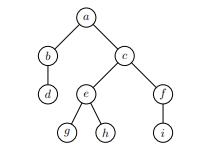
\includegraphics[width=10cm,height=10cm]{treeA.png} \\
 
 Beispiel für eine maximal unabhängige Menge: M={c,d,g,h,i}

\paragraph{b)} 
Beschreiben Sie einen Algorithmus mit Dynamischem Programmieren, der eine maximale unabhängige Menge von $T$ berechnet. \\

First we develop an algorithm to calculate the number of nodes in a maximum independent set. To this end we use variables $v.max$, which will contain the number of nodes of a maximum independent set of the subtree rooted at a node $v \in V$. For our algorithm we observe the following. For a node $v \in V$, there are two possibilities: \\

\subparagraph{1.}
Either v is int the independent set. In this case no children of v can be in the independent set, but the children of the children of v can. Thus, if the grandchildren of v are $w_{1} ... w_{k}$ we conclude

$$v.max=1+ \sum^{k}_{i=1} w_{i}.max$$

in this case assuming that we already know the values $w_{i}.max$ for all $i=1 ... k$.

\subparagraph{2.}
Otherwise v is not contained in the independent set. In this case the children of v might be in the independent set. Let $c_{1} ... c_{l}$ be the children of v. Then we have

$$v.max= \sum^{l}_{i=1}c_{i}.max.$$

To calculate the maximum set of v, we have to use the possibility, where we can obtain the higher value for v.max: 

$$c.max=max { \sum^{l}_{i=1} c_{i}.max.1 + \sum^{k}_{i=1} w_{k}.max}$$

\textbf{SizeMaxIndependentSet(T)} \\
\begin{algorithm}[H]
\SetAlgoLined
 // initizalize v.max to 0 for all nodes in the tree T: \\
\While {not all nodes of T are visited in a post-order walk}{
  \eIf {e has no children}{
  v.max $\leftarrow$ 1 \;
  } {
  \eIf{v has no grandchildren}{
  v.max $\leftarrow \sum c.max$ 
  } {
  v.max $\leftarrow max {\sum c.max.1 + \sum w.max}$
  }}
}
\end{algorithm} \\

\textbf{MaxIndependentSet(T)} \\
\begin{algorithm}[H]
\SetAlgoLined
// initialize an empty set M \\
// initialize an empty list l and insert the root of T into it: \\
\While {l is not empty}{
v $\leftarrow$ first element of l \;
delete the first element of l \;
\eIf {r has no children }{
  M $\leftarrow M \cup {r}$ \; 
} {
  \eIf{r has no grandchildren}{
    M $\leftarrow M \cup {c, c is child of r}$ \; 
  } { \eIf {r.max = $\sum c.max$} {
         append all children of r to l \;
  } {
  M $\leftarrow M \cup {r}$ \; 
  append all grandchildren of r to l \;
  }
  }
}
}
\Return M
\end{algorithm} \\

\paragraph{c)}
 Begründen Sie die Korrektheit Ihres Algorithmus. \\
 
\paragraph{d)}
 Wie ist die Laufzeit Ihres Verfahrens? \\

%----------------------------------------------------------------------------
\subsection{Dynamisches Prog.: Palindrom}
Ein \emph{Palindrom} ist eine Zeichenfolge, die vorwärts und rückwärts gelesen gleich ist. Beispiele für Palindrome sind alle Zeichenfolgen
der Länge 1, \texttt{KAJAK}, \texttt{REITTIER}, \texttt{SEI FIES} und \texttt{DREH MAL AM HERD}.

\smallskip\noindent
Gegeben sei eine Zeichenfolge $S[1..n]$. Eine \emph{Teilfolge} $S'$ von $S$ besteht aus Buchstaben,
die in $S'$ in der selben Reihenfolge auftreten wie in $S$. Zum Beispiel ist
\texttt{ATMEN} eine Teilfolge von \texttt{ALGORITHMEN}. Das \emph{längste Palindrom} in $S$ ist
die längste Teilfolge von $S$, die ein Palindrom darstellt.

\paragraph{a)}
Geben Sie einen Algorithmus in Pseudocode an, der die Länge des längste Palindrom in $S$ berechnet. Verwenden Sie dabei Dynamische Programmierung. \\

\textbf{Länge des längsten Palindrom} \\
\begin{algorithm}[H]
\SetAlgoLined
\KwIn{String S}
\KwOut{int Länge des längsten Palindroms in S}
 // löschen aller Leerzeichen \\
\For {I=1 ... length(S)}{
 \If {i-tes Zeichen von S ist Leerzeichen}{
 S $\leftarrow$ konkateniere die ersten i-1 Zeichen von S mit den letzten length(S)-i Zeichen
 }
}
int i $\leftarrow$ 1 \\
int j $\leftarrow$ length(S) \\
\Return LLPWorker(S,i,j)
\end{algorithm} \\

\textbf{LLPWorker} \\
\begin{algorithm}[H]
\SetAlgoLined
\KwIn{String S, int i, int j}
\KwOut{int Länge des längsten Palindroms in S}
 // nur ein Zeichen $\rightarrow$ palindromisch\\
\If {i == y}{
  \Return 1
}

// nur 2 gleiche Zeichen $\rightarrow$ palindromisch\\
\If {length(S) == 2 und S[i] == S[j]}{
  \Return 2
} 

// erstes und letztes Zeichen gleich \\
\If {S[i] == S[j]}{
  \Return LLPWorker(S, i+1,j-1) +2
}

// erstes und letztes Zeichen verschieden \\
\Return max(LLPWorker(S,i,j-1),LLPWorker(S,i+1,j))
\end{algorithm} \\

\textbf{max} \\
\begin{algorithm}[H]
\SetAlgoLined
\KwIn{int x, int y}
\KwOut{int (max von a und b)}
\eIf {a > b}{
  \Return a
}{
  \Return b
}
\end{algorithm} \\

\paragraph{b)}
Begründen Sie die Korrektheit und die Laufzeit Ihres Algorithmus aus (a). \\

\textbf{Korrektheit} \\
Zuerst müssen alle Leerzeichen aus dem Ausgabestring gelöscht werden. Für die beiden trivialen Fälle liefert unser Algorithmus das richtige Ergebnis, da alle Wörter der Länge 1 palindromisch sind und ein Wort der Länge 2 ebenfalls palindromisch ist, falls die Zeichen übereinstimmen. Wenn die Zeichen aber verschieden sind und wir noch ein Wort der Länge 2 haben so landen wir im 4.Fall, so wird das Maximum aus dem längsten Palindrom zweier einbuchstabiger Wörter gebildet.

Um den dritten Fall zu erklären, wo das erste und letzte Zeichen identisch sind, müssen wir LLPWorker, auf den String zwischen dem ersten und letzten Zeichen, aufrufen und 2 addieren. 

Beim letzten Fall, sind das erste und das letzte Zeichen verschieden, d.h. sie verlängern nicht die Länge des Polyndroms. Also überprüfen wir das Maximum aus den LLPWorker von dem String aus dem ersten Zeichen bis zum vorletzten Zeichen und dem LLPWorker vom String vom 2. Zeichen bis zum letzten. \\

\textbf{Laufzeit} \\
\begin{itemize}
\item Leerzeichen löschen mit Laufzeit $O(n)$
\item LLPWorker 
  \begin{itemize}
  \item 1.Fall 
  T(1)=1
  \item 2.Fall
  T(2)=1
  \item 3.Fall
  T(n-2)
  \item 4.Fall
  T(n-1)
  \end{itemize}
Um also die Laufzeit für den worst case abschätzen zu können, brauchen wir eigentlich nur den 4. Fall anschauen, so das der String sozusagen immer weiter in den 4.Fall kommt und die Zeichen nicht identisch werden. \\

Daraus folgt das Rekursionsschema:
$$T(n)=2T(n-1)$$
$$=2*2T(n-2)$$
$$=2*2*2T(n-3)$$
$$=2^{i}*T(n-i)$$

Jetzt brauchen wir das Rekursionsende:
$$T(n)_{n-2}=2^{n-2}T(n-(n-2))=2^{n-2}T(n-n+2)=2^{n-2}T(2)=2^{n-2}$$ \\

D.h. wir gehen von einer Laufzeit von $O(2^{n-2}) \in O(2^{n})$ aus.
\end{itemize}

\paragraph{c)}
Geben Sie einen Algorithmus in Pseudocode an, der mit Hilfe von (a) das längste Palindrom in $S$ berechnet und
begründen Sie die Korrektheit und die Laufzeit Ihres Algorithmus. \\

\paragraph{d)}
Demonstrieren Sie die Funktionsweise Ihrer Algorithmen an der Zeichenfolge \texttt{DADBBCAA}. \\

%----------------------------------------------------------------------------------------
\newpage
\section{Blatt 09}
%----------------------------------------------------------------------------
\subsection{Dynamisches Programmieren}
Seien $u,v,w \in \Sigma^*$ Wörter über einem  Alphabet $\Sigma$. Wir nennen $w$ \textit{einen Shuffle} aus $u$ und $v$, wenn es eine Zerlegung $u=u_1\dots u_k$ und $v=v_1\dots v_l$ gibt mit $u_i, v_j\in \Sigma^*$ für alle $i,j$, so dass $w=u_1v_1u_2v_2\dots$ ist.\\
Zum Beispiel ist $w=\mathit{INaFOlgoRMrithAmTIenK}$ ein Shuffle aus den Wörtern $u=\mathit{INFORMATIK}$ und $v=\mathit{algorithmen}$.

\paragraph{a)}
Geben Sie einen Algorithmus an, der für drei gegebene Wörter $u,v,w$ unter der Verwendung von dynamischer Programmierung entscheidet, ob $w$ ein Shuffle aus $u$ und $v$ ist. \\

Algorithmus testet, ob $w \backslash u = v$, also die Symbole von u werden abgeleitet von links nach rechts, dabei werden all diese Symbole aus w entfernt. Nach Abarbeitung von u, muss w=v gelten, falls w Shuffle war. u,v,w werden als Array repräsentiert. \\

\textbf{checkShuffle(w,u,v)} \\
\begin{algorithm}[H]
\SetAlgoLined
\For {i=0; $i < length(u)$; i++}{
 delete($u[i],w$)
 \eIf {$w 0 0 v$}{
   \Return true \;
 } {
   \Return false \;
 }
}
\end{algorithm} \\

\textbf{delete($u[i],w$)} \\
\begin{algorithm}[H]
\SetAlgoLined
j = 0 \\
\While {$j < length(w)$} {
  \If {$u[i]= = w[j]$} {
    \For {k=j;$k < length(w)-1$; k++} {
      $w[j]=w[j+1]$ \;
    }
    \Return checkShuffle(w,u,v)
  }
  j++
  \Return false \;
}
\end{algorithm} \\

\paragraph{b)} 
Geben Sie die Laufzeit in Abhängigkeit der Längen der Wörter an. \\

Beim Algorithmus wir u einmal komplett durchlaufen ($O(lenght(u))$), wobei zwischen jedem Schritt, w entweder komplett durchlaufen wird und Ende oder in w das Symbol aus u gefunden in maximal length(w) Schritten. \\
Da nun length(w) bei gefundenen Symbol von u in w nicht um 1 verringert, wird length(w) jeden Schritt bei der Abarbeitung von u, wird im nächsten Schritt immer nur die Teilwertlänge von v weitergelaufen, welche zwischen 1 und lenght(v) liegt. Im worst case haben wir also $O(length(u))+O(length(v))$ und die $O(length(w))$ entspricht mit length(w)=n erhalten wird $O(n)$ Laufzeit (mit Faktor $c \leq 1$). 

%----------------------------------------------------------------------------
\subsection{Programmieraufgabe}
Laden Sie die Java-Vorlage aus dem Moodle herunter und implementieren Sie die folgenden Methoden:

\paragraph{a)}
 \texttt{isShuffled(String w, String u, String v)}, die entscheidet ob das Wort $w$ ein Shuffle aus den zwei Wörtern $u$ und $v$ ist. \\
 
\paragraph{b)}
 \texttt{isShuffled(String w, String u, String v, String z)}, die entscheidet of das Wort $w$ ein Shuffle aus den drei Wörtern $u$, $v$ und $z$ ist.

%----------------------------------------------------------------------------
\subsection{Anagramme}
Seien $u$ und $v$ zwei Wörter über einem endlichen Alphabet $\Sigma$. Ein Anagramm eines Wortes $u$ ist ein Wort $v$, das aus einer Permutation der Buchstaben von $u$ gebildet werden kann.

\paragraph{a)}
Welche Eigenschaften muss eine Hashfunktion erfüllen, um Anagramme schnell identifizieren zu können? \\

Für jedes Symbol/ Buchstabe aus Wort muss ein individueller Wert existieren (Zahlenwert). Zusätzlich darf/ sollte keiner dieser Werte aus der Summe anderer Werte entstehen (Wertunabhängigkeit).

\paragraph{b)} 
Die Funktion \texttt{getBytes} weißt jedem Buchstaben aus $\Sigma$ eine eindeutige natürliche Zahl zu. Betrachte folgende Hashfunktion $h\colon \Sigma^* \rightarrow \mathbb N$
$$h(w_1\dots w_n)= \sum \limits_{i=1}^n \mathtt{getBytes}(w_i)$$
Zeigen Sie, dass die Hashfunktion $h$ zwei Anagramme auf denselben Hashwert abbildet. \\

Da $h(w_{1}, ..., w_{n})= \sum^{n}_{i=1} getBytes(w_{i})$ gilt und $\sum^{n}_{i=1} getBytes(w_{i})=w_{1}+...+w_{n}$, so ist nach Kommutativgesetz die Reihenfolge der Summanden für den Ergebniswert irrelevant, so das alle Permutationen derselbe Summand zum selben Wert führen. \\

$\Rightarrow$ Zwei Argumente bilden auf denselben Wert ab, da ihre Summanden gleich sind.

\paragraph{c)} 
Warum ist die Funktion dennoch ungeeignet, um Anagramme zu filtern? Welche Strings werden noch auf dieselben Hashwerte abgebildet? \\

Da zwei Hashwerte summiert den Hashwert eines anderen Symbols erzeugen können, kann z.B. $h(w_{1},w_{2},w_{3})=h(w_{1},w_{4})$ gelten, falls $w_{2}+w_{3}=w_{4}$. Unterschiedliche Werte können also denselben Hashwert erzeugen.

\paragraph{d)}
Modifizieren Sie die Hashfunktion so, dass sie sich besser dazu eignet Anagramme zu filtern. Begründen Sie, warum sich Ihre neue Hashfunktion besser verhalten sollte und zeigen Sie, dass sie immer noch zwei Anagramme auf denselben Wert abbildet. \\

Wähle als Hashwert für einzelne Symbole Primzahlen. \\
$getBytes(w_{i})$ soll also für alle existierende Symbole eine Primzahl sein. Da Summen von Primzahlen immer eindeutig sind. (Beweis: Primfaktorzerlegung, Multiplikationen sind vor Schreibweise für Addition)

%----------------------------------------------------------------------------
\subsection{Hashing}
Betrachten Sie die folgende Hashfunktion

\begin{align*}
  h_{a,b,m}\colon\ \ &\rightarrow \{0,\dots, m-1\}\\
  x &\mapsto( a x +b) \bmod m
\end{align*}

und die Eingabewerte
$$S = \{13,45,64,78,116\}\enspace.$$

\paragraph{a)}
 Geben Sie Werte für $a$, $b$ und $m$ an, sodass

\subparagraph{i.)}
 alle Werte aus $S$ auf den selben Hashwert abgebildet werden. \\
  \begin{itemize}
 \item a=0
 \item b=4
 \item m=3
 \end{itemize} \\
 
 Dann ist $h_{0,4,3}(x)$ eine Konstante, die alle Werte auf 4 mod 3 = 1 abbildet.
 
\subparagraph{ii.)}
alle Werte aus $S$ auf unterschiedliche Hashwerte abgebildet werden. \\
 \begin{itemize}
 \item a=1
 \item b=0
 \item m=10
 \end{itemize} \\
 
 Dann ist $h_{1,0,10}(13)=3$ , $h_{1,0,10}(45)=5$, $h_{1,0,10}(64)=4$, $h_{1,0,10}(78)=8$ und $h_{1,0,10}(116)=6$, also alles verschiedene Werte.    

\paragraph{b)} 
Sei $g_i(x) \; {\color{darkgray}:=(}  h_{1,0,5}(x) + i) \bmod 5$. Geben Sie jeweils die Hashtabelle an, die entsteht, wenn $S$ in aufsteigender Reihenfolge in eine zuvor leere Hashtabelle eingefügt wird. Verwenden Sie dabei die folgenden Kollisionsauflösungsstrategien:

\subparagraph{i.)}
Verkettetes Hashing mit der Hashfunktion $g_0$ \\

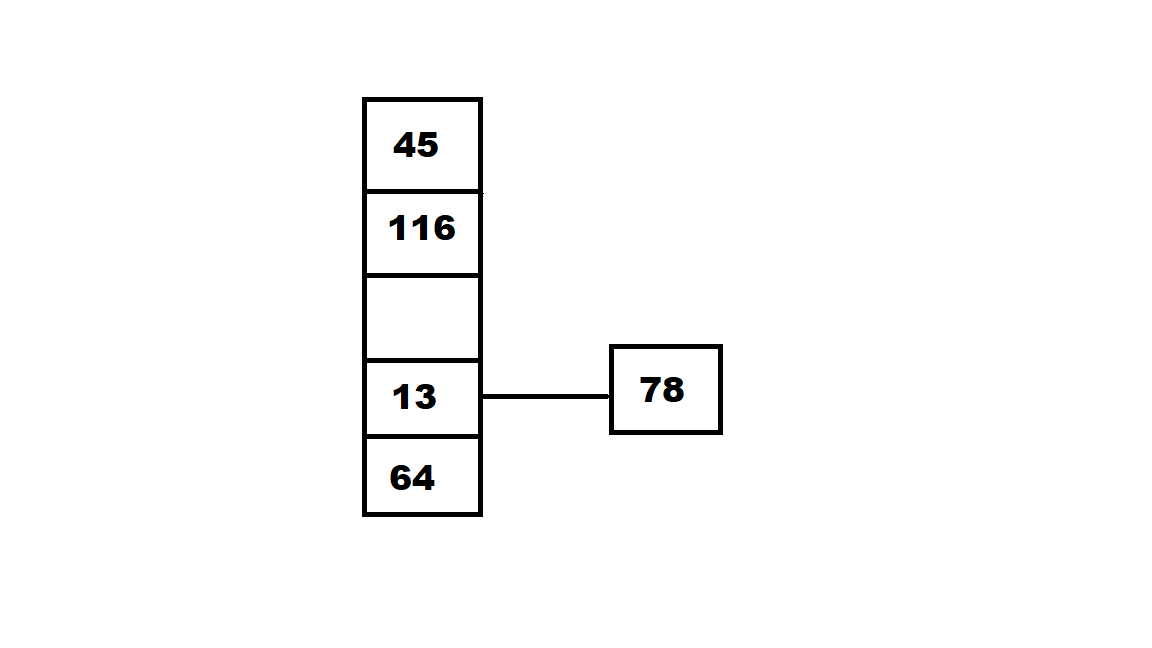
\includegraphics[width=10cm,height=5cm]{hashbi.png} \\

\subparagraph{ii.)}
Hashing mit offener Adressierung mit ${(g_i)}_{i\geq 0}$ \\

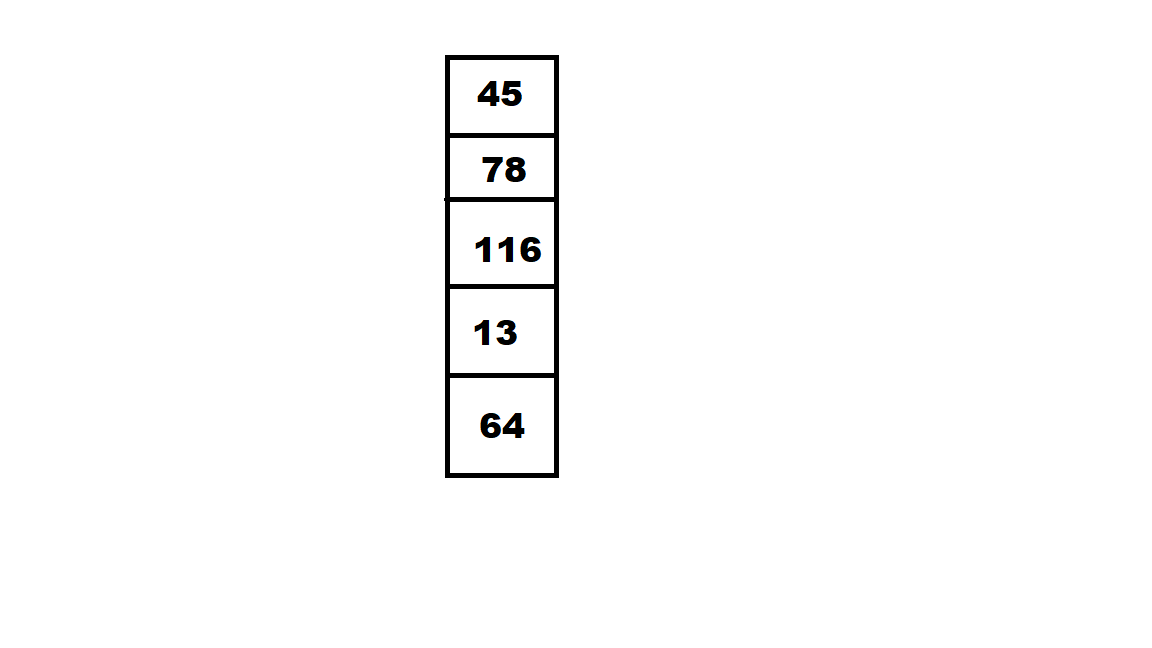
\includegraphics[width=10cm,height=5cm]{hashbii.png} \\

\paragraph{c)}
 Zeigen Sie, dass es für alle Werte von $a$ und $b$ bei $m=5$ zu Kollisionen kommt. \\
 
 Beweis: \\
 Seien a und b beliebig \\
 Umformen der mod-Rechenregeln: \\
 $h_{a,b,5}(x)=(a*x+b) mod 5 = (((a*x) mod 5) +b) mod 5$ \\
 $= (((x*a) mod 5)+b) mod 5 = ((((x mod 5)*a) mod 5) +b) mod 5$ \\
 Einmaliges Einsetzen für x die Werte 13 und 78 \\
 zz. das folgende Gleichung für alle a,b gilt : \\
 $((((13 mod 5)*a) mod 5)+b) mod 5 =((((78 mod 5)*a) mod 5)+b) mod 5$ \\
 $\Leftrightarrow (((3*a) mod 5)+b) mod 5 = ((((3*a) mod 5)+b) mod 5$ \\
 
 Es gibt also unendlich viele Lösungen für diese Gleichung, d.h. diese gilt für alle a,b. Daraus folgt, dass es immer zur Kollision bei $m=5$ kommt. \\
 
\paragraph{d)} 
Geben Sie Werte für $a$, $b$ und $m$ an, sodass $m$ minimal ist und alle Werte aus $S$ auf unterschiedliche Hashwerte abgebildet werden. \\
 \begin{itemize}
 \item a=1
 \item b=0
 \item m=6
 \end{itemize} \\
 
 Kontrolle:
  \begin{itemize}
 \item 13 mod 6 =1
 \item 45 mod 6 = 3
 \item 64 mod 6 = 4
 \item 78 mod 6 = 0
 \item 116 mod 6 = 2
 \end{itemize} \\
 
 Man sieht, dass $m=6$ minimal ist, da wir bei $m=5$ in c) gesehen haben, dass es da nicht möglich war und das es bei kleineren m's auch nicht möglich wäre, da man dann auf zu wenigen unterschiedlichen Fächern abbilden könnte.
 
%----------------------------------------------------------------------------------------
\newpage
\section{Blatt 10}
%----------------------------------------------------------------------------
\subsection{Grapheigenschaften}
Gegeben sei ein einfacher, zusammenhängender Graph $G=(V,E)$ mit $|V|=n$ und $|E|=m$. \\

G=(V,E) einfach zusammenhängend \\
$|V|=n$ Knoten \\
$|E|=m$ Kanten 

\paragraph{a)}
Zeigen Sie, dass es in $G$ zwei Knoten mit demselben Grad gibt. \\

G hat zwei Knoten vom selben Grad ]]
$|V| = n$, maximaler Grad p Knoten: n-1; minimaler Grad: 1 \\
$\rightarrow$ Schubladenprinzip : $\dfrac{n}{n-1} Fächer \rightarrow Doppelbelegung$

\paragraph{b)}
Zeigen Sie, dass $G$ eine gerade Anzahl an Knoten mit ungeradem Grad hat. \\

G hat eine gerade Anzahl von Knoten mit ungeradem Grad \\
$\sum^{v \in V}_{v} deg(v) = 2*|E| \Rightarrow \sum_{v,even} deg(v) + \sum_{v,odd} deg(v)=2*|E| \Leftrightarrow \sum_{v,odd} deg(v) = 2*|E| * \sum_{v,even} deg(v)$

\paragraph{c)}
$G$ heiß \emph{vollständig}, wenn jeder Knoten durch Kanten mit jedem anderen Knoten
verbunden ist. Berechnen Sie die Anzahl der Kanten in einem vollständigen Graphen. \\

Jeder Knoten hat n-1 Verbindungen $n*n-1$ \\
ABER jede Kante ist mit zwei Knoten verbunden deshalb gilt: $\dfrac{n*n-1}{2}$

\paragraph{d)}
$G$ heißt \emph{$d$-regulär}, wenn jeder Knoten aus $V$ einen Grad von $d$ hat.
Zeigen Sie, dass $m=\tfrac{d\cdot n}2$, falls $G$ $d$-regulär ist. \\

d regulär $\Rightarrow$ deg(v) = d $\forall v \in V$ \\
$\sum_{v} deg(v)= 2* |E|$ \\
$n*d= 2*|E|$ \\
$\dfrac{n*d}{2}=|E|=m$

%----------------------------------------------------------------------------
\subsection{Adjazenzmatrix vs. Adjazenzliste}
Sei $G=(V,E)$ der folgende gerichtete Graph:

\begin{figure}[h]
	\centering
	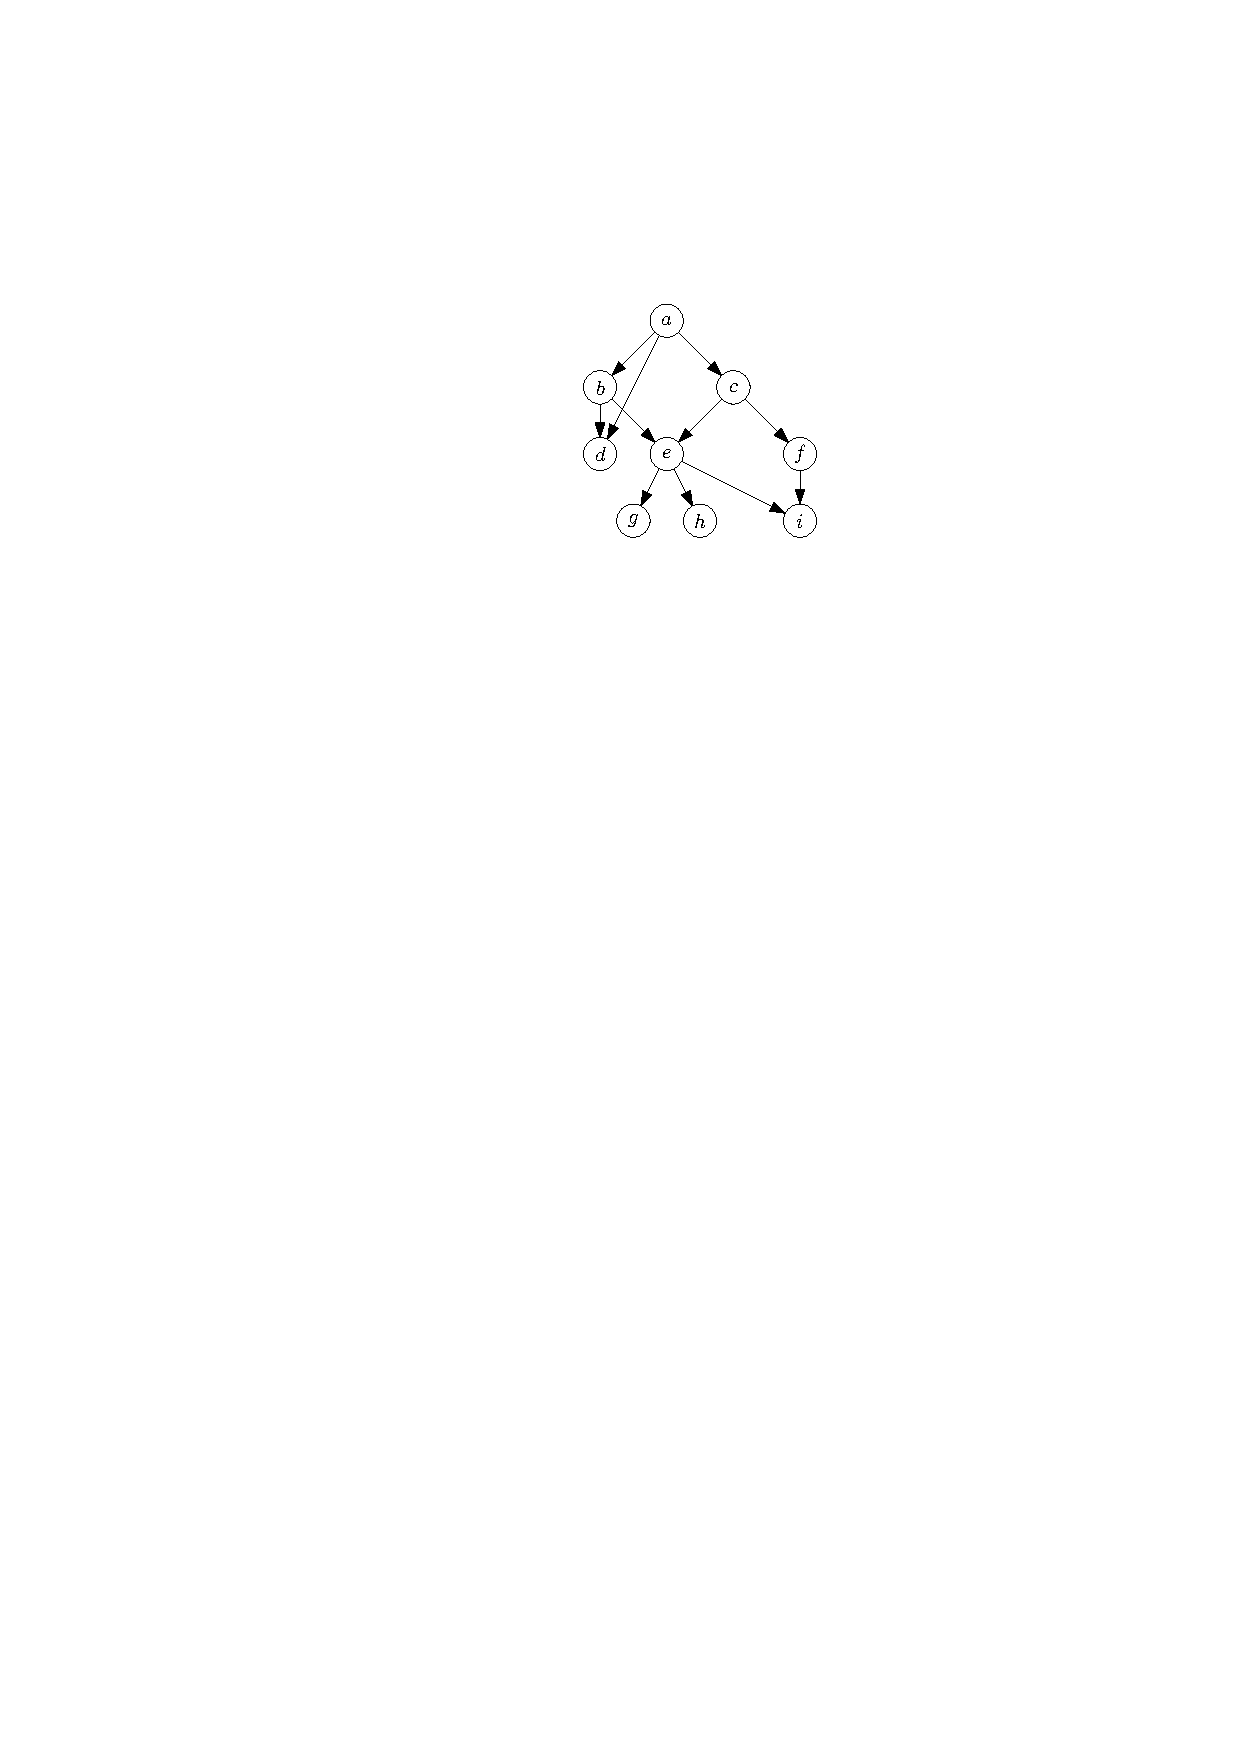
\includegraphics[scale=0.9]{graph}
\end{figure}

\paragraph{a)}
Berechnen Sie die Adjazenzmatrix und die Adjazenzliste für $G$. \\

\begin{tabular}{|c|c|}
\hline
Adjazenzliste & Adjazenzmatrix \\\hline
a $\rightarrow$ b $\rightarrow$ c $\rightarrow$ d & 0111 0000 0 \\\hline
b $\rightarrow$ d $\rightarrow$ e                & 0001 1000 0\\\hline
c $\rightarrow$ e $\rightarrow$ f                & 0000 1100 0\\\hline
d                                              & 0000 0000 0\\\hline
e $\rightarrow$ g $\rightarrow$ h $\rightarrow$ i & 0000 0011 1\\\hline
f $\rightarrow$ i                               & 0000 0000 1\\\hline
h                                              & 0000 0000 0\\\hline
i                                              & 0000 0000 0\\\hline
\end{tabular}

\paragraph{b)}
Wenden Sie den Algorithmus aus der Vorlesung auf Ihre Adjazenzliste aus (a) an,
um eine topologische Sortierung von $G$ zu berechnen. \\

Reihenfolge: abcdefghi \\
Laufzeit: $O(n^{2})$ \\

\begin{center}
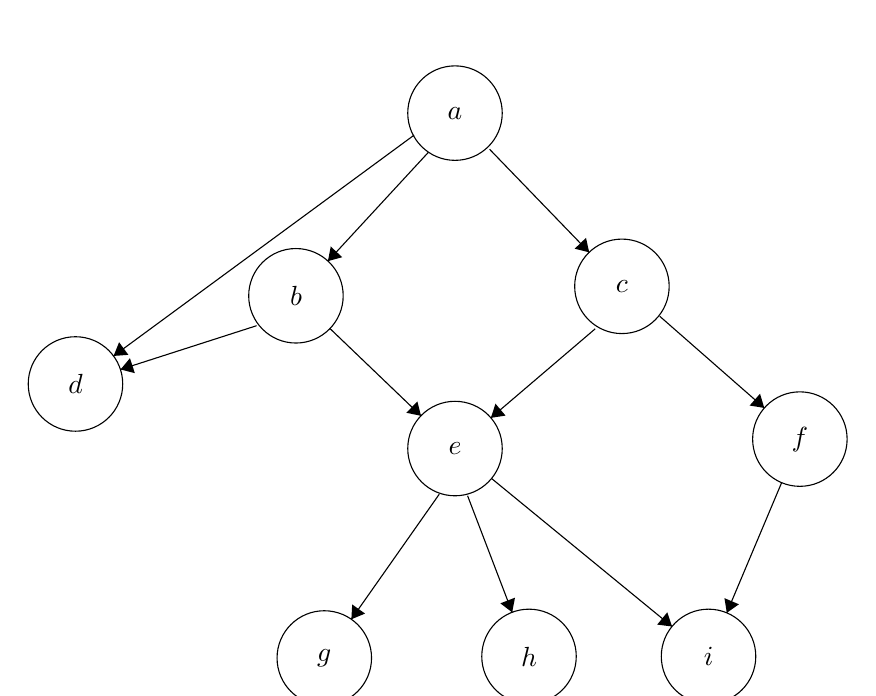
\begin{tikzpicture}[scale=0.2]
\tikzstyle{every node}+=[inner sep=0pt]
\draw [black] (38.4,-16) circle (3);
\draw (38.4,-16) node {$a$};
\draw [black] (28.3,-27.6) circle (3);
\draw (28.3,-27.6) node {$b$};
\draw [black] (49,-27) circle (3);
\draw (49,-27) node {$c$};
\draw [black] (14.3,-33.2) circle (3);
\draw (14.3,-33.2) node {$d$};
\draw [black] (38.4,-37.3) circle (3);
\draw (38.4,-37.3) node {$e$};
\draw [black] (60.3,-36.7) circle (3);
\draw (60.3,-36.7) node {$f$};
\draw [black] (30.1,-50.6) circle (3);
\draw (30.1,-50.6) node {$g$};
\draw [black] (43.1,-50.5) circle (3);
\draw (43.1,-50.5) node {$h$};
\draw [black] (54.5,-50.5) circle (3);
\draw (54.5,-50.5) node {$i$};
\draw [black] (36.7,-18.5) -- (30.33,-25.4);
\fill [black] (30.33,-25.4) -- (31.24,-25.15) -- (30.51,-24.47);
\draw [black] (40.6,-18.3) -- (46.92,-24.84);
\fill [black] (46.92,-24.84) -- (46.72,-23.92) -- (46,-24.61);
\draw [black] (35.8,-17.4) -- (16.72,-31.42);
\fill [black] (16.72,-31.42) -- (17.66,-31.35) -- (17.07,-30.55);
\draw [black] (25.8,-29.5) -- (17.16,-32.28);
\fill [black] (17.16,-32.28) -- (18.07,-32.51) -- (17.76,-31.56);
\draw [black] (30.46,-29.68) -- (36.24,-35.22);
\fill [black] (36.24,-35.22) -- (36.01,-34.31) -- (35.31,-35.03);
\draw [black] (47.3,-29.7) -- (40.68,-35.35);
\fill [black] (40.68,-35.35) -- (41.61,-35.21) -- (40.97,-34.45);
\draw [black] (51.4,-28.9) -- (58.04,-34.72);
\fill [black] (58.04,-34.72) -- (57.77,-33.82) -- (57.11,-34.57);
\draw [black] (59.14,-39.47) -- (55.66,-47.73);
\fill [black] (55.66,-47.73) -- (56.43,-47.19) -- (55.51,-46.8);
\draw [black] (40.72,-39.2) -- (52.18,-48.6);
\fill [black] (52.18,-48.6) -- (51.88,-47.7) -- (51.24,-48.48);
\draw [black] (39.2,-40.3) -- (42.03,-47.7);
\fill [black] (42.03,-47.7) -- (42.21,-46.77) -- (41.28,-47.13);
\draw [black] (37.4,-40.2) -- (31.82,-48.14);
\fill [black] (31.82,-48.14) -- (32.69,-47.78) -- (31.87,-47.2);
\end{tikzpicture}
\end{center}

\paragraph{c)}
Der \emph{transponierte Graph} eines Graphen $G=(V,E)$ ist der Graph $G'=(V,E')$, wobei
\[ E' := \{ (v,u) \mid (u,v)\in E\}. \]
Nehmen Sie an, dass $G$ als Adjazenzmatrix vorliegt. Beschreiben Sie einen Algorithmus,
der den transponierten Graph $G'$ in einer Laufzeit von $\calO(|V|^2)$ berechnet. \\

transponieren der Matrix mit 2 For-Schleifen \\

\paragraph{d)}
Nehmen Sie nun an, dass $G$ als Adjazenzliste vorliegt. Beschreiben Sie einen Algorithmus,
der den transponierten Graph $G'$ in einer Laufzeit von $\calO(|V| + |E|)$ berechnet. \\

Sei $n= |V|$ \\
Sei L Adjeszenzliste für Knoten \\
i: $L[i]$ enthält Adjeszenztenknoten von i \\

\begin{algorithm}[H]
\SetAlgoLined
initialisiere L' für alle Knoten \\
\For {i= 1 to n}{
  \For {j= 1 to $|L[i]|$} {
     \If {$L[i]$ enthält j}{
       $L'[j]$.append i
     }
  }
}
\end{algorithm} \\

%----------------------------------------------------------------------------
\subsection{Dijkstra-Algorithmus}
Wenden Sie den Dijkstra-Algorithmus auf das folgende Beispiel an.
Verwenden Sie dabei $s$ als Startknoten und
geben Sie alle Zwischenschritte an!

\begin{figure}[h!]
	\centering
	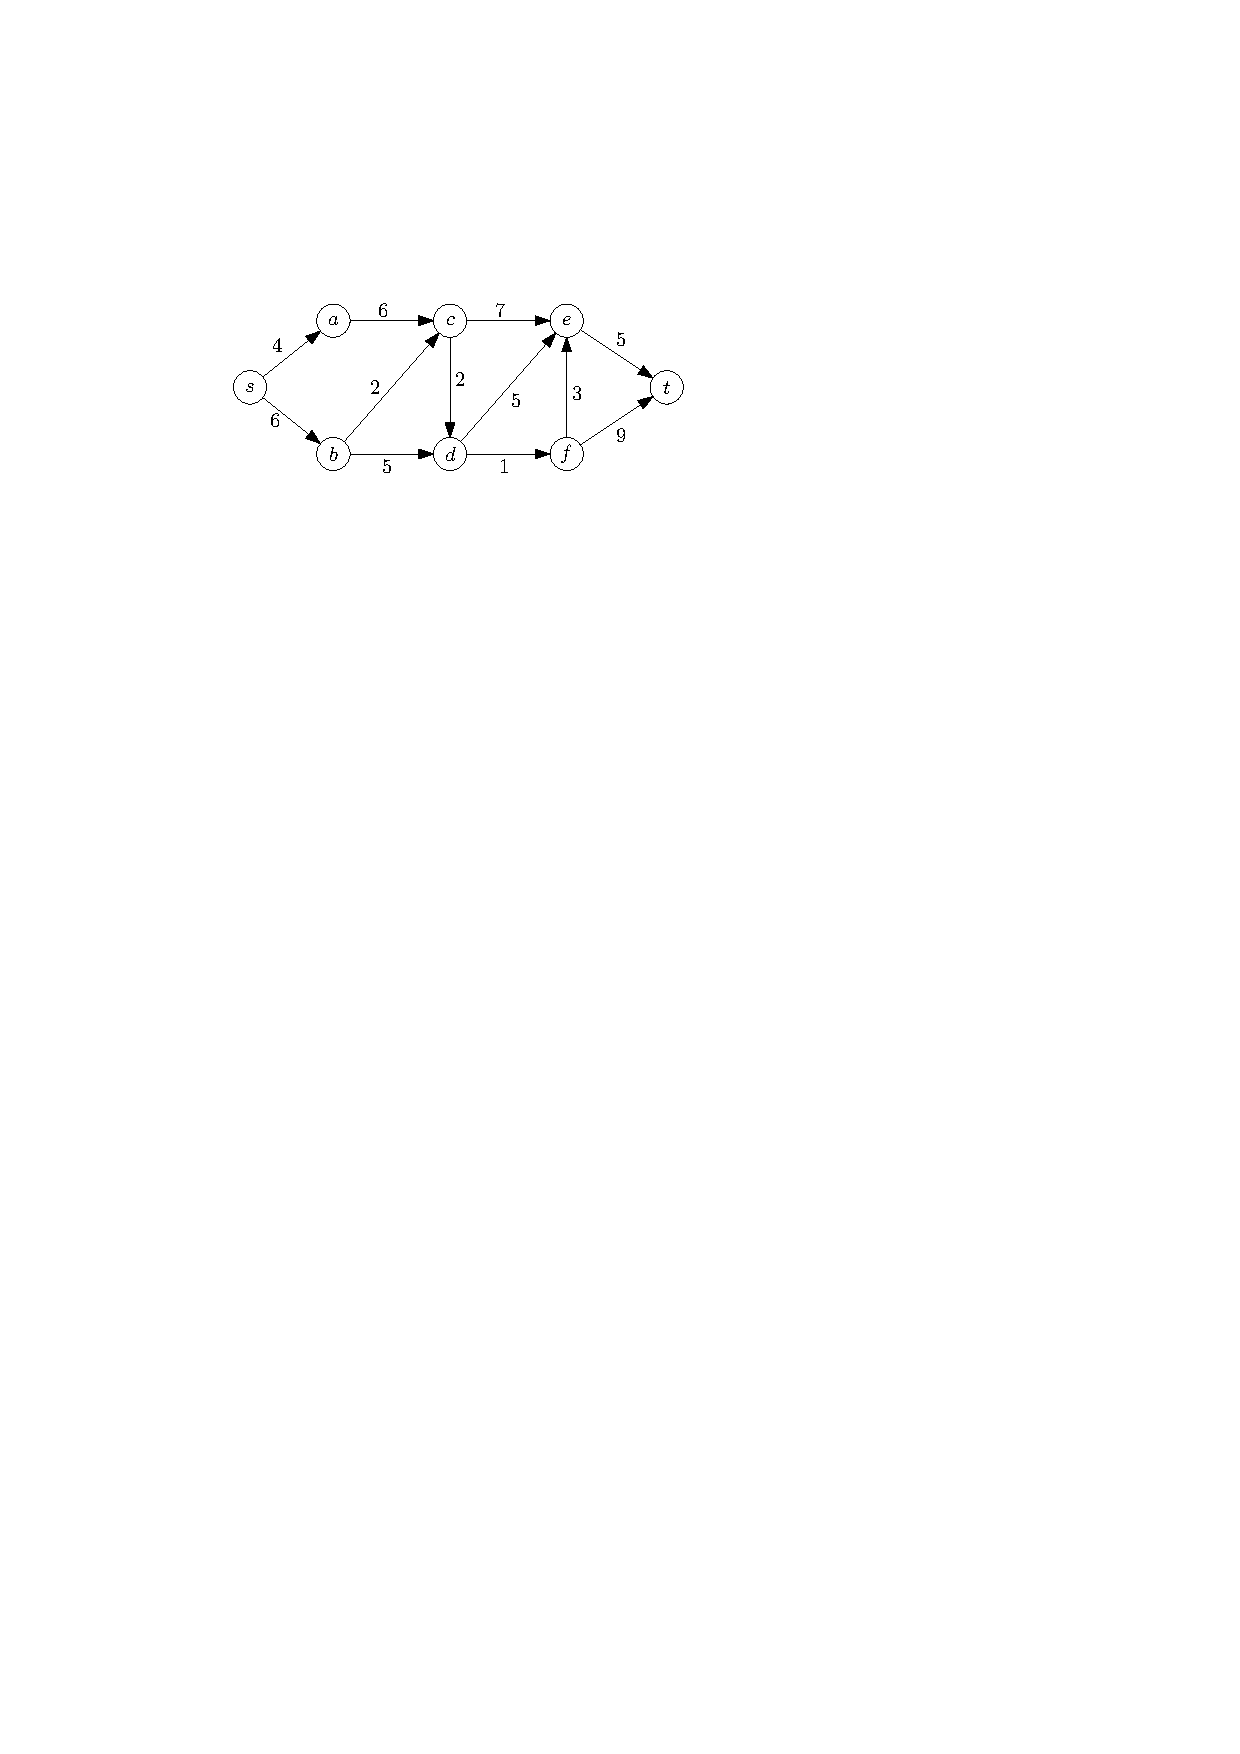
\includegraphics[scale=0.9]{dijkstra}
\end{figure}

\begin{tabular}{|c||c|c|}
\hline
# & s & s' \\\hline
1 & (s,0,-) & (a,4,s),(b,6,s) \\\hline
2 & (a,4,s) & (b,6,s),(i,10,a) \\\hline
3 & (b,6,s) & (c,8,b),(d,11,b) \\\hline
4 & (c,8,b) & (d,10,c),(e,15,c) \\\hline
5 & (d,10,c) & (f,11,d),(e,15,c) \\\hline
6 & (f,11,d) & (e,14,f),(t,20,f) \\\hline
7 & (e,14,f) & (t,19,e) \\\hline
\end{tabular}

%----------------------------------------------------------------------------
\subsection{Anwendung von Dijkstra}
Betrachten Sie ein gerichtetes Netzwerk $G=(V,E)$ zusammen mit einer
Wahrscheinlichkeitsfunktion $p:E\rightarrow (0,1]$. Dabei ist $0<p(v,w) \le 1$
die \emph{Zuverlässigkeit} der Kante $(v,w)$.
Seien $s,t\in V$ Knoten, zwischen denen ein Packet gesendet werden soll.
Ob das Packet erfolgreich gesendet wird, hängt von der Zuverlässigkeit
des verwendeten Pfades ab. Dabei beschreibt die \emph{Zuverlässigkeit eines Pfades}
die Wahrscheinlichkeit, dass ein Packet erfolgreich über einen Pfad gesendet
werden kann.

\paragraph{a)}
Wie lässt sich die Zuverlässigkeit eines Pfades $s=v_0\to v_1\to \cdots \to v_k=t$
berechnen? \\

$$\prod^{k}_{i=1} p(v_{i-1},v_{i})$$

\paragraph{b)}
Geben Sie ein Beispiel an, bei dem der Dijkstra-Algorithmus nicht den Pfad von $s$ nach $t$ mit der höchsten Zuverlässigkeit findet, wenn man für jede Kante $(v,w)$
das Kantengewicht $1-p(v,w)$ (d.\,h. die Ausfallswahrscheinlichkeit) verwendet. \\

\begin{center}
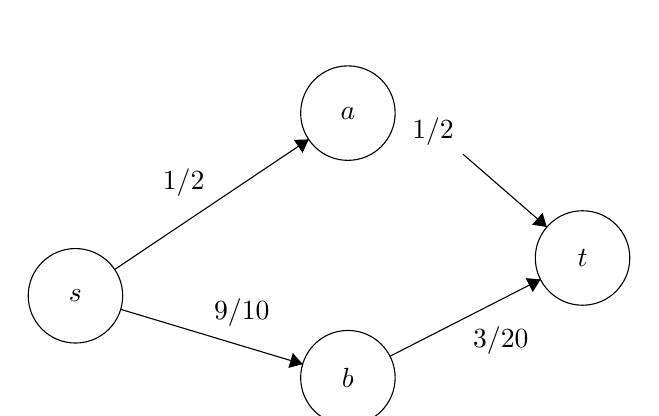
\begin{tikzpicture}[scale=0.2]
\tikzstyle{every node}+=[inner sep=0pt]
\draw [black] (17.6,-35.6) circle (3);
\draw (17.6,-35.6) node {$s$};
\draw [black] (34.9,-24) circle (3);
\draw (34.9,-24) node {$a$};
\draw [black] (34.9,-40.8) circle (3);
\draw (34.9,-40.8) node {$b$};
\draw [black] (49.8,-33.2) circle (3);
\draw (49.8,-33.2) node {$t$};
\draw [black] (20.09,-33.93) -- (32.41,-25.67);
\fill [black] (32.41,-25.67) -- (31.47,-25.7) -- (32.02,-26.53);
\draw (24.47,-29.3) node [above] {$1/2$};
\draw [black] (20.47,-36.46) -- (32.03,-39.94);
\fill [black] (32.03,-39.94) -- (31.4,-39.23) -- (31.12,-40.18);
\draw (28.16,-37.59) node [above] {$9/10$};
\draw [black] (37.57,-39.44) -- (47.13,-34.56);
\fill [black] (47.13,-34.56) -- (46.19,-34.48) -- (46.64,-35.37);
\draw (44.61,-37.51) node [below] {$3/20$};
\draw [black] (42.2,-26.6) -- (47.53,-31.23);
\draw (41.66,-25.15) node [left] {$1/2$};
\fill [black] (47.53,-31.23) -- (47.26,-30.33) -- (46.6,-31.09);
\end{tikzpicture}
\end{center}

\begin{center}
\begin{tikzpicture}[scale=0.2]
\tikzstyle{every node}+=[inner sep=0pt]
\draw [black] (17.6,-35.6) circle (3);
\draw (17.6,-35.6) node {$s$};
\draw [black] (34.9,-24) circle (3);
\draw (34.9,-24) node {$a$};
\draw [black] (34.9,-40.8) circle (3);
\draw (34.9,-40.8) node {$b$};
\draw [black] (49.8,-33.2) circle (3);
\draw (49.8,-33.2) node {$t$};
\draw [black] (20.09,-33.93) -- (32.41,-25.67);
\fill [black] (32.41,-25.67) -- (31.47,-25.7) -- (32.02,-26.53);
\draw (24.47,-29.3) node [above] {$1/2$};
\draw [black] (20.47,-36.46) -- (32.03,-39.94);
\fill [black] (32.03,-39.94) -- (31.4,-39.23) -- (31.12,-40.18);
\draw (28.16,-37.59) node [above] {$1/10$};
\draw [black] (37.57,-39.44) -- (47.13,-34.56);
\fill [black] (47.13,-34.56) -- (46.19,-34.48) -- (46.64,-35.37);
\draw (45.11,-37.51) node [below] {$17/20$};
\draw [black] (44.2,-28) -- (47.6,-31.16);
\draw (43.67,-26.54) node [left] {$1/2$};
\fill [black] (47.6,-31.16) -- (47.36,-30.25) -- (46.68,-30.98);
\end{tikzpicture}
\end{center}

\begin{itemize}
\item Pfad s-a-t: Kosten 1
\item Pfad s-b-t: Kosten $\dfrac{19}{20}$
\end{itemize}

\paragraph{c)}
Beschreiben Sie einen Algorithmus, der mit Hilfe des Dijkstra-Algorithmus,
den Pfad zwischen $s$ und $t$ mit der höchsten Zuverlässigkeit findet. Begründen Sie
die Laufzeit und Korrektheit Ihres Algorithmus. \\

\begin{enumerate}
\item Wie bekommen wir Add? \\
$log(a*b)=log(a)+log(b)$
\item Wie minimieren? \\
Gewicht: $-log(p(v,w))$
\end{enumerate}

%----------------------------------------------------------------------------------------
\newpage
\section{Blatt 11}
%----------------------------------------------------------------------------
\subsection{Algorithmenentwurf}
Sei $G = (V,E)$ ein gerichteter Graph. Der Graph $G$ heisst \emph{$(s,t)$-Graph}, falls er nur eine \emph{Quelle} und nur eine \emph{Senke} hat, wobei ein Knoten Quelle (Senke) heisst, falls er keine eingehenden Kanten hat (nur eingehende Kanten hat).

\medskip\noindent
Nehmen Sie an, dass der Graph $G$ in Adjazenzlistendarstellung gegeben ist.
Geben Sie einen Algorithmus in Pseudocode, der in Zeit $\calO(|V| + |E|)$ feststellt, ob $G$ ein $(s,t)$-Graph ist. \\

\begin{algorithm}[H]
\SetAlgoLined
\For {every node in G}{
incomingDegree(node) = 0 \;
}
sinks = 0; \\
\For {every node in G}{
  \For {every target node in nod.adjacentlist}{
  comingDegree(targetNode) = incomingDegree(targetNode) + 1 \;
     \If {node.adjacentNodes is empty}{
     sinks++ \;
     }
  }
}
sources = 0; \\
\For {every node in G}{
   \If {incomingDegree(node) == 0}{
   sources++ \;
   }
}
\If {Sources == 1}{
   \If {sinks ==1}{
     \Return true \;
   }
}
\Return false;
\end{algorithm} \\

%----------------------------------------------------------------------------
\subsection{Maximum Bottleneck Path}
Sei $G=(V,E,c)$ ein gerichteter Graph mit positiven Kantenkosten $c$. Sei $P$ ein Pfad zwischen zwei Knoten $u$ und $v$, wobei die billigste Kante in $P$ Kosten $k$ habe. $P$ heißt \emph{breitester Pfad} von $u$ nach $v$, wenn es keinen anderen Pfad in $G$ von $u$ nach $v$ gibt, dessen billigste Kante teurer als $k$ ist.

\paragraph{a)}
Zeichnen Sie in folgendem Graphen den breitesten Pfad von $s$ nach $t$ ein. \\

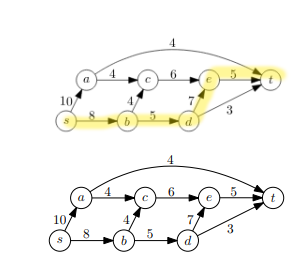
\includegraphics[width=7cm,height=7cm]{graph112.png} \\

\paragraph{b)} 
Modifizieren Sie Dijkstras Algorithmus so, dass er zu einem gegebenen Startknoten $s$ die breitesten Pfade zu allen anderen Knoten findet. Begründen Sie die Korrektheit und die Laufzeit Ihres Algorithmus. \\

\begin{algorithm}[H]
\SetAlgoLined
visited = {s} \\
queue = empty maxHeap sorted by broadestWidth \\
\textbf{Forall} $(s,v) \in E$ \textbf{do} \\
broadestPathTo(v) = $\{(s,v) \}$ \;
broadestWidth(v) = c(s,v) \;
queue.add(v) \;
\textbf{end} \\
\textbf{Forall} $v \in V | (s,v) \notin E$ \textbf{do} \\
broadestPathTo(v) = $ \{ \}$ \;
broadestWidth(v) = 0 \;
\textbf{end} \\
\While {visited != V}{
   currentNode = queue.removeMax() \;
   visited = visited $\cup$ currentNode \;
   \textbf{forall} $(currentNode, next) \in E$ \textbf{do} \\
      \If {$next \notin queue$}{
         queue.add(next) \;
      }
      minNewWidth = min(broadestWidth(currentNode), c(currentNode, next)) \;
      \eIf {broadestPathTo(next) == $\{ \}$}{
         broadestPathTo(next) = broadestPathTo(currentNode) $\cup$ (currentNode,next) \;
         broadestWidth(next) = minNewWidth \;
      } {
         \If {minNewWidth $>$ broadestWith(next)}{
           broadestPathTo(next) = broadestPathTo(currentNode) $\cup$ (currentNode,next) \;
           broadestWidth(next) = minNewWidth \;
         }
      }
   \textbf{end} \\
}
\textbf{forall} $v \in V$ \textbf{do} \\
   \Return (v,broadestWidth(v), broadestPathTo(v)) \;
\textbf{end}   
\end{algorithm} \\

\textbf{Korrektheit:} \\
Unser Algorithmus geht wie der Dijkstra-Algorithmus vor. Es liefert das korrekte Ergebnis, da sich ein Pfad durch das Hinzufügen von Kanten nur verschmälern, aber nicht verbreitern kann. D.h. der lokal breiteste Pfad ist auch der global breiteste Pfad. \\

\textbf{Laufzeit:} 
\begin{itemize}
\item while-Schleife: $O(|V|)$
\item forall-Schleife: $O(|E|)$
\item queue enthält maximal $|V|$ Knoten, d.h. einfügen, sortieren und max entfernen kostet jeweils $O(log|V|)$
\item einfügen von $|V|$ Knoten in queue, entfernen von $|V|$ Knoten, updaten des Sortierkriterium um $O(|E|)$
\item Laufzeit beträgt: $O(|V|)+O(|E|)+O(2*|V|+|E|)*O(log(|V|)) = O((|V|+|E|)log(|V|))$
\end{itemize}

%----------------------------------------------------------------------------
\subsection{Bellman/Ford-Algorithmus}
Gegeben sei folgender gerichteter Graph $G=(V,E)$. Lösen Sie mit Hilfe des Bellman-Ford-Algorithmus das \textit{single-source shortest-paths} Problem für den Source-Knoten $s$.
Verwenden Sie dabei die folgende Reihenfolge für die Kanten:
\[ (s,a), (s,c), (s,d), (a,b), (a,d), (b,a), (c,d), (d,b), (d,e), (e,b). \]
Zeigen Sie alle Zwischenschritte! \\

\textbf{Durchlauf 1:} \\

\begin{tabular}{|c||c|c|c|}
\hline
Kante(u,v) & (Distanz(u)+Gewicht(u,v) $<$ Distanz(v)) & Distanz(v) & Vorgänger(v) \\
\hline \hline
(s,a) & true & 1 & s \\\hline
(s,c) & true & 2 & s \\\hline
(s,d) & true & 2 & s \\\hline
(a,b) & true & 0 & a \\\hline
(a,d) & false & 2 & s \\\hline
(b,a) & false & -1 & b \\\hline
(c,d) & false & 2 & s \\\hline
(d,b) & false & -4 & d \\\hline
(d,e) & true & 6 & d \\\hline
(e,b) & false & -4 & d \\\hline
\end{tabular} \\

\textbf{Durchlauf 2:} \\

\begin{tabular}{|c||c|c|c|}
\hline
Kante(u,v) & (Distanz(u)+Gewicht(u,v) $<$ Distanz(v)) & Distanz(v) & Vorgänger(v) \\
\hline \hline
(s,a) & false & 1 & s \\\hline
(s,c) & false & 2 & s \\\hline
(s,d) & false & 2 & s \\\hline
(a,b) & false & 0 & a \\\hline
(a,d) & false & 2 & s \\\hline
(b,a) & true & -2 & b \\\hline
(c,d) & false & 2 & s \\\hline
(d,b) & false & -4 & d \\\hline
(d,e) & false & 6 & d \\\hline
(e,b) & false & -4 & d \\\hline
\end{tabular} \\

\textbf{Durchlauf 3:} \\

\begin{tabular}{|c||c|c|c|}
\hline
Kante(u,v) & (Distanz(u)+Gewicht(u,v) $<$ Distanz(v)) & Distanz(v) & Vorgänger(v) \\
\hline \hline
(s,a) & false & 1 & s \\\hline
(s,c) & false & 2 & s \\\hline
(s,d) & false & 2 & s \\\hline
(a,b) & false & 0 & a \\\hline
(a,d) & true & 1 & a \\\hline
(b,a) & false & -2 & b \\\hline
(c,d) & false & 2 & s \\\hline
(d,b) & true & -5 & d \\\hline
(d,e) & true & 5 & d \\\hline
(e,b) & false & -5 & d \\\hline
\end{tabular} \\

\textbf{Durchlauf 4:} \\

\begin{tabular}{|c||c|c|c|}
\hline
Kante(u,v) & (Distanz(u)+Gewicht(u,v) $<$ Distanz(v)) & Distanz(v) & Vorgänger(v) \\
\hline \hline
(s,a) & false & 1 & s \\\hline
(s,c) & false & 2 & s \\\hline
(s,d) & false & 2 & s \\\hline
(a,b) & false & 0 & a \\\hline
(a,d) & false & 1 & a \\\hline
(b,a) & true & -3 & b \\\hline
(c,d) & false & 2 & s \\\hline
(d,b) & false & -5 & d \\\hline
(d,e) & false & 5 & d \\\hline
(e,b) & false & -5 & d \\\hline
\end{tabular} \\

\textbf{Durchlauf 5:} \\

\begin{tabular}{|c||c|c|c|}
\hline
Kante(u,v) & (Distanz(u)+Gewicht(u,v) $<$ Distanz(v)) & Distanz(v) & Vorgänger(v) \\
\hline \hline
(s,a) & false & 1 & s \\\hline
(s,c) & false & 2 & s \\\hline
(s,d) & false & 2 & s \\\hline
(a,b) & false & 0 & a \\\hline
(a,d) & true & 0 & a \\\hline
(b,a) & false & -3 & b \\\hline
(c,d) & false & 2 & s \\\hline
(d,b) & true & -6 & d \\\hline
(d,e) & true & 4 & d \\\hline
(e,b) & false & -6 & d \\\hline
\end{tabular} \\

\textbf{Durchlauftest auf negativen Zykel} \\

\begin{tabular}{|c||c|c|c|}
\hline
Kante(u,v) & (Distanz(u)+Gewicht(u,v) $<$ Distanz(v)) & Distanz(u) & Distanz(v) \\
\hline \hline
(s,a) & false & 0 & -3 \\\hline
(s,c) & false & 0 & 2 \\\hline
(s,d) & false & 0 & 0 \\\hline
(a,b) & false & -3 & -6 \\\hline
(a,d) & false & -3 & 0 \\\hline
(b,a) & true ($\Rightarrow$ break) & -6 & -3 \\\hline
(c,d) &  & 2 & 0 \\\hline
(d,b) &  & 0 & -6 \\\hline
(d,e) &  & 0 & 4 \\\hline
(e,b) &  & 4 & -6 \\\hline
\end{tabular} \\


%----------------------------------------------------------------------------
\subsection{Floyd/Warshall-Algorithmus}
Sei $G=(V,E)$ ein gerichteter Graph. Die \emph{transitive Hülle} $G'=(V,E')$ des
Graphen $G$, ist der Graph mit Schleifen, der folgendermaßen definiert ist:

\begin{center}
$(u,v)\in E'$ gdw. $u=v$ oder es gibt einen Pfad von $u$ nach $v$ in $G$.
\end{center}

\paragraph{a)}
Berechnen Sie die transitive Hülle des folgenden Graphen. \\

$G' = (V,E')$ mit E' \\
$= \{(1,1),(2,1),(2,2),(2,3),(2,4),(3,1),(3,2),(3,3),(3,4),(4,1),(4,2),(4,3),(4,4) \}$

\paragraph{b)}
Modifizieren Sie den Algorithmus von Floyd/Warshall, um die transitive Hülle $G'$ eines Graphen $G$ in $\calO(n^3)$ zu berechnen. Begründen Sie die Korrektheit und die Laufzeit Ihres Algorithmus.

\begin{algorithm}[H]
\SetAlgoLined
A ist Adjazenzmatrix von G = (V,E) \\
$n=|V|$ \\
baue neue Matrix(n x n) M \\
\For {i= 1 to n}{
   \For {j= 1 to n}{
      M[i][j] = A[i][j] \;
   }
} 
\For {i = 1 to n}{
   M[i][i] = 1 \;
}
\For {k= 1 to n}{
   \For {i=1 to n}{
      \For {j= 1 to n}{
         \If {M[i][k] == 1 $&&$ M[k][j] == 1}{
            M[i][j] = 1 \;
         }
      }
   }
}
\Return H 
\end{algorithm} \\

\textbf{Korrektheit:} \\
Jeder Knoten enthält eine Kante zu sich selbst (transitive Hülle), siehe Zeile 9-11. Außerdem übernimmt die transitive Hülle auch die bereits vorhandenen Kanten des Graphen. Der FW-Algorithmus prüft nun für jeden Knoten, ob die bisher berechnetete Distanz zwischen den Knotenpaaren kürzer wird. Da wir aber nur binär Denken müssen, es also nur 0 keinen Pfad gibt und 1 es gibt einen Pfad, entsteht nur eine neue Adjazenzmatrix. \\

\textbf{Laufzeit:} \\
ineinander geschachtelte For-Schleifen mit Laufzeit je $O(|V|)$, d.h. die Laufzeit des Algorithmus beträgt: $O(|V|^{3})$

%----------------------------------------------------------------------------
\subsection{Programmieraufgabe: Dijkstra-Algorithmus}
Laden Sie die Java-Vorlage aus dem Moodle herunter und machen Sie sich mit der Implementierung von Graphen vertraut, die Sie in der Vorlage finden. Implementieren Sie dann die Methode:

\begin{center}
\texttt{runDijkstra(Graph g, Node start)},
\end{center}

\noindent die den Dijkstra-Algorithmus ausführen soll.
Verwenden Sie bei Ihrer Implementierung sinnvolle Variablennamen und kommentieren Sie Ihren Code!
Laden Sie Ihre Lösung ins Moodle. Nicht kompilierende Abgaben werden \textbf{mit 0 Punkten} bewertet.

%----------------------------------------------------------------------------------------
\end{document}